

\chapter{Absztrakt}

A hipergráfok gyakran alkalmazott matematikai eszközök az informatika számos területén, így a szemantikus web, bioinformatika, szenzorhálózatok, adatbázisrendszerek, szociális hálózatok, gépi látás és egyéb részterületek számos megoldása épül rájuk.
Ezen feladatok vizsgálata során különösen hasznos lehet a hipergráfok ábrázolása. Vizualizáció során egyszerre merül fel igény a mögöttes struktúra tökéletes leképezésére, a könnyű értelmezhetőségre (így esztétikai és ergonómiai metrikákra), az általános alkalmazhatóságra, gyors futásidőre és - ezzel összefüggésben - a megjeleníthető adathalmaz méretének maximalizálására is, továbbá gyakran felmerül a dinamikus környezet feladatok kezelésének problémája is.


Mint látható, ez egy felettébb összetett problémát eredményez, amely megoldására számos módszer született már a szakterületi irodalomban, azonban ezek gyakran szenvednek egy -- vagy több -- tervezési elv sérülésétől, így egyik sem terjedt el a gyakorlatban.
Jelen dolgozatban különböző optimalizációs módszerek, illetve heurisztikák teljesítményét vizsgáljuk a fenti szempontok alapján, különös tekintettel az általános alkalmazhatóságra és a szemantikailag helyes leképezésre.

%\cleardoublepage
\chapter{Elméleti alapok}
\label{ch:intro}

\section{A dolgozat felépítése}

Segítendő a szövegben való tájékozódást, ebben az alfejezetben részletezem a dolgozat felépítését. A szöveg két fő fejezetre bontható, amelyek előtt egy rövid összefoglaló (Absztrakt), után pedig egy összefoglaló fejezet (Konklúzió) található. Az első (Elméleti alapok című) fejezetben először megadom a probléma leírásához, illetve megértéséhez szükséges definíciókat és fogalmakat, majd a tágabb és szűkebb problématerület irodalmi áttekintésére kerül sor, az általam kitűzött pontos feladat megfogalmazásával lezárva. Az első fejezet második felében a megoldás során alkalmazott módszerek elméleti alapjait tekintem át. A második fejezet (Saját eredmények) az általam vizsgált különböző megoldási módszereket írja, illetve ezek teljesítményét vizsgálja különböző paraméterek mellett, továbbá a levont következtetésekre is itt térek ki.

\begin{note}
A dolgozatban szereplő egyes szakszavak (néha egész szakterületek) egyáltalán nem, vagy nem elég hangsúlyosan szerepelnek a magyar szakirodalomban ahhoz, hogy elterjedt fordításuk legyen. Ezekben az esetekben -- további figyelmeztetés nélkül -- az angol nyelvű megfelelőjüket fogom használni. Népszerű, szinonímaként használt szakkifejezéseket igyekszem per jellel elválasztva felsorolni.
\end{note}

\section{Probléma}

\subsection{Alapdefiníciók}

Ahhoz, hogy megértsük a megoldandó problémát, számos fogalmat át kell tekintsünk először.

\subsubsection{Gráfok}

A gráf (variációi) alapvető fontosságú adattípus(ok) a modern informatikai megoldások során. Definiálásuk nem csak a dolgozat későbbi részeiben felbukkanó algoritmusok miatt fontos, hanem a -- gyakran a gráfok általánosításának tekintett -- hipergráfok mélyebb megértését is elősegíti. 

\begin{definition}
\textbf{Irányítatlan gráfnak} nevezünk egy olyan, rendezett $G=(V,E)$ párt, ahol $V$ egy nem-üres halmaz, $E$ pedig egy olyan multihalmaz, amely a $V$ elmeiből képzett kételemű halmazokat tartalmaz. Formálisan $E \subseteq \{\{u,v\} | u,v \in V\}$. A $V$ halmazt \textbf{csúcshalmaznak} is szokás nevezni, elemeit \textbf{csúcsoknak}, míg $E$-t az \textbf{élhalmaz}, elemeit pedig \textbf{él} névvel illetjük. Az élek által tartalmazott elemeket az adott él \textbf{végpontjainak} hívjuk. Két csúcs \textbf{szomszédos}, ha van olyan él $G$-ben, amely őket tartalmazza, míg egy csúcs \textbf{izolált}, ha egyetlen élnek sem végpontja. A $G'=(V',E'), V' \subseteq V, E' \subseteq E$ a $G=(V,E)$ gráf \textbf{részgráfja}.
\end{definition}

\begin{definition}
Egy nem-üres halmazból, $V$-ből, és az elemeiből képzett \textit{rendezett párokat} tartalmazó $A$ multihalmazból képzett rendezett $D=(V,A)$ párt \textbf{irányított gráfnak} hívjuk. Az irányítatlan gráfok nómenklatúrája itt is érvényes, azonban az élek rendezett párjában az első elemet speciálisan \textbf{kiindulópontnak}, a másodikat pedig \textbf{végpontnak} is szokás nevezni. Azt mondjuk, hogy egy $(u, v) \in A$ él az $u$ csúcsnak egy \textbf{kimenő éle}, $v$-nek egy \textbf{bemenő éle}. \textbf{Forrásnak} nevezzük azt a csúcsot, amelynek nincsenek bemenő élei, \textbf{nyelőnek} azt, aminek nincsenek kimenő élei.
\end{definition}

\begin{definition}
Az $e_i, e_j \in E, i \neq j$ éleket \textbf{párhuzamos éleknek} nevezzük, ha $e_i=e_j$. \textbf{Hurokélnek} egy olyan élet nevezünk, amely $\{v, v\}$ vagy $(v, v)$ formájú, azaz a két végpontja azonos.
\end{definition}

\begin{definition}
A $v \in V$ él \textbf{fokszámát} $d$-vel jelöljük, azaz $d=| \{ e | e \in E \land v \in e \}|$. A $G$ gráf \textbf{k-reguláris}, ha minden csúcsának fokszáma $k$. Irányított gráf esetében megkülönbeztetjük a \textbf{befokszámot} és a \textbf{kifokszámot}.
\end{definition}

\begin{definition}
\textbf{Egyszerű gráf} egy olyan irányítatlan gráf, amelyben sem párhuzamos, sem hurokélek nincsenek jelen.
\end{definition}

\begin{definition}
\textbf{Páros gráfnak} hívunk egy $G=(V,E)$ gráfot, ha $V=A \cup B, A \cap B = \emptyset$ és sem $A$-n, sem $B$-n belül nem fut él. Jelölése: $G=(A,B)$ vagy $G=(A,B,E)$.
\end{definition}

\begin{definition}
Irányított gráf esetén élek egy $(u_1, v_1), \ldots, (u_k, v_k)$ sorozatát \textbf{sétának} nevezzük, ha $v_i=u_{i+1}, i=1 \ldots k-1$. Irányítatlan gráfok esetén analóg módon defináljuk a fogalmat, azonban eltekintünk a csúcsok élen belüli sorrendjétől. Ha a séta semelyik két éle nem tartalmazza ugyanazt a csúcsot, akkor a sétát \textbf{útnak} mondjuk. Ha egyedül a séta kezdőpontja egyezik meg a végpontjával, akkor az egy \textbf{kör}. Két csúcs \textbf{távolsága} a köztük lévő legrövidebb útban szereplő élek száma, ha ilyen nincs, akkor végtelen. Egy $v$ csúcs \textbf{elérhető} az $s$ csúcsból, ha a távolsága nem végtelen tőle. \textbf{Összefüggőnek} mondott egy gráf (vagy részgráf), ha abban minden csúcs elérhető mindegyik másikból, míg egy \textbf{összefüggő komponens} a vizsgált gráf csúcsainak egy olyan részhalmaza, amely összefüggő, de nem bővíthető úgy, hogy az maradjon.
\end{definition}

\begin{note}
Irányítatlan gráfokban az elérhetőség ekvivalens az összefüggőséggel, így lineáris időben megkapható. (A linearis futásidő elérhető irányított gráfokra is.)
\end{note}

\begin{definition}
$K_n$-nel jelöljük az $n$ csúcsú egyszerű gráfot, amelyben minden csúcspár között fut él, az ilyen gráfok neve \textbf{teljes gráf}. Mikor csak egy részgráfra igaz ez a tulajdonság, akkor azt \textbf{teljes részgráfnak} vagy \textbf{klikknek} mondjuk.
\end{definition}


\begin{definition}
\textbf{Topologikus sorrendként} ismert a $D=(V,A)$ irányított gráf csúcsainak egy olyan sorrendje, ahol minden csúcsból csak nála nagyobb sorszámúba megy él. A topologikus sorrend megléte ekivivalens azzal, hogy az adott gráfban nincsen kör, így az ilyet \textbf{körmentes gráfnak} nevezzük.
\end{definition}

\begin{definition}
Egy $G=(V,E)$ irányítatlan gráf \textbf{line graphja} alatt az $L(G)=(E, \{ \{ e_i, e_j \} | \exists v \in V : v \in e_i \land v \in e_j, i \neq j \})$ irányítatlan gráfot értjük.
\end{definition}

\subsubsection{Halmazrendszerek és hipergráfok}

Mint az absztraktban is említettem, halmazalapú adatreprezentációkkal, így hipergráfokkal és halmazrendszerekkel az informatika számos területén találkozhatunk. Az egyes problématerületek -- sőt, gyakran az egy problématerületet vizsgáló különböző szakcikkek -- azonban egymással konkuráló definíciókat alkalmaznak a hipergráfokra. Sokszor a halmazrendszerek szinonímájának tekintik a fogalmat, míg például -- a szakterület egyik alapművének számító -- Hypergraphs c. \cite{berge_hypergraphs_book} kötet mind az általunk használt -- mindjárt megismertetett -- definícióhoz, mind a halmazrendszer alapúhoz képest megszorításokat vezet be.

\begin{definition}
A $H$ halmaz \textbf{hatványhalmaza} $\mathcal{P}(H) = \{x | x \subseteq H\}$, azaz a $H$ halmaz összes részhalmazainak halmaza.
\end{definition}

\begin{definition}
A $H$ halmaz fölötti $\mathcal{F}$ \textbf{halmazrendszert} $\mathcal{F} \subseteq \mathcal{P}(H)$-ként definiáljuk.
\end{definition}

\begin{definition}
Ebben a dolgozatban \textbf{irányítatlan hipergráf} vagy egyszerűen hipergráf alatt egy olyan, rendezett $H=(V,E)$ párt értünk, ahol $V$ a \textbf{(hiper)csúcsok} nem-üres halmaza, míg $E$, a \textbf{hiperélek} halmaza, egy olyan multihalmaz, amelynek az elemei $\mathcal{P}(V) \setminus \emptyset$-ből kerülnek ki.
\end{definition}

\begin{note}
A hipergráf, úgy is ismertek, mint a gráfok általánosításai, ahol minden hiperél pontosan 2 elemet tartalmaz, azaz 2-reguláris. Egyrészről ez jól láthatóan függ a választott gráf-, és hipergráfdefinícióktól. Az itt használt definíciók alapján hipergráfok nem tartalmazhatnak hurokéleket, viszont párhuzamos éleket igen, így nem tökéletes általánosításai az irányítatlan gráfoknak, viszont irányítatlan egyszerű gráfoknak már igen.
\end{note}

\begin{note}
Egy másik felmerülő kérdés a hipergráfok kapcsán a hiperutak, más szóval a tranzitivitás fogalma a hiperélek között. A szakirodalomban erre is több, azonban jobban elkülönülő definíció létezik. Az itt bemutatott eredmények nem építenek a tranzitív relációra, így tetszőleges definíció tételezhető fel.
\end{note}

\subsubsection{Gráf- és hipergráf-adatszerkezetek} \label{adsDefinitions}

Gráfok gépi kezelésére köztes gráfreprezentációkra, gráfadatszerkezetekre van szükség. Leggyakrabban az adjacencia mátrix, az incidencia mátrix, az éllista és a ritka reprezentációk általános osztálya használatos. Mivel a megoldások során csak az első kettőt alkalmazzuk, ezért a többit itt nem is definiálom.

\begin{definition}
A $G=(V,E)$ gráf \textbf{adjacencia mátrixa} alatt azt a $|V| \times |V|$ méretű $A_G$ mátrixot értjük, amelyben $a_{ij}=1$, ha $\{v_i, v_j\} \in E$, egyébként 0.
\end{definition}

\begin{definition}
A $G=(V,E)$ gráf \textbf{incidencia mátrixa} alatt azt a $|V| \times |E|$ méretű $I_G$ mátrixot értjük, amelyben $i_{jk}=1$, ha $v_j \in e_k$, egyébként 0.
\end{definition}

\begin{definition}
A $H=(V,E)$ hipergráf \textbf{incidencia mátrixát} ugyanúgy definiáljuk, ahogy a gráfokon értelmezett megfelelőjét.
\end{definition}

\begin{note}
Hipergráfok esetében az adjacencia mátrix nem értelmezett.
%, azonban a szakirodalomban gyakran használnak gráfokat köztes reprezentációként, így (az incidencia mátrixon kívül) a bipartite incidence structure, a multimodal/multi-layer/multiplex/multidimensional graph/network és a line/intersection graph fogalmaknak érdemes utánanéznie az ez iránt érdeklődő olvasónak.
\end{note}

\begin{definition}
A $H=(V,E)$ hipergráf \textbf{line/intersection graphja} az $L(H)=(E, \{ \{ e_i, e_j \} | e_i \cap e_j \neq \emptyset, i \neq j \})$ képlettel kapott egyszerű gráfot fedi. Jól látható, hogy ez általánosítása a gráfok esetében alkalmazott definíciónak.
\end{definition}

\begin{definition}
A $H=(V,E_H)$ hipergráf \textbf{bipartite incidence structure-e} alatt azt a $G=(A,B,E_G)$ páros gráfot értjük, amelyben $A=V, B=E_H$ és $E_G=\{\{u,v\} | u \in V, v \in E_H, u \in v \}$.
\end{definition}

\begin{definition}
Egy irányítatlan $H=(V_H,E_H)$ hipergráf \textbf{(szuper)duálisa} az a $G=(V_G,E_G)$ egyszerű gráf, amelyben $V_G=\{X | X \subseteq E_H \land \exists v \in V_H : ((\forall e \in X: v \in e) \land (\forall e \notin X : v \notin e) \}$ és $E_G=\{\{X,Y\} | X,Y \subseteq E_H, X \neq Y \land \exists v \in V_H : (v \in X \land v \in Y)\}$
\end{definition}

\begin{note}
Figyeljük meg, hogy a szuperduálisban szereplő csúcsok száma exponenciális az eredeti csúcshalmaz tekintetében!
\end{note}

\subsection{Gráfok ábrázolása} \label{graphLayout}

Mivel a gráfok gyakran használt, könnyen konceptualizálható modellek, ezért a számítógépes vizsgálat mellett gyakran előnyös a felhasználó számára vizualizálni őket. Gráfok reprezentálhatók halmazokként vagy numerikusan (például adjacencia mátrixként), azonban ember-gép interakciók során a leggyakrabban olyan képként szokás ábrázolni őket, amelyen a csúcsok köröknek, az őket összekötő élek pedig egyenes (egyes esetekben akár görbe) vonalaknak felelnek meg.

\begin{figure}[H]
	\centering
	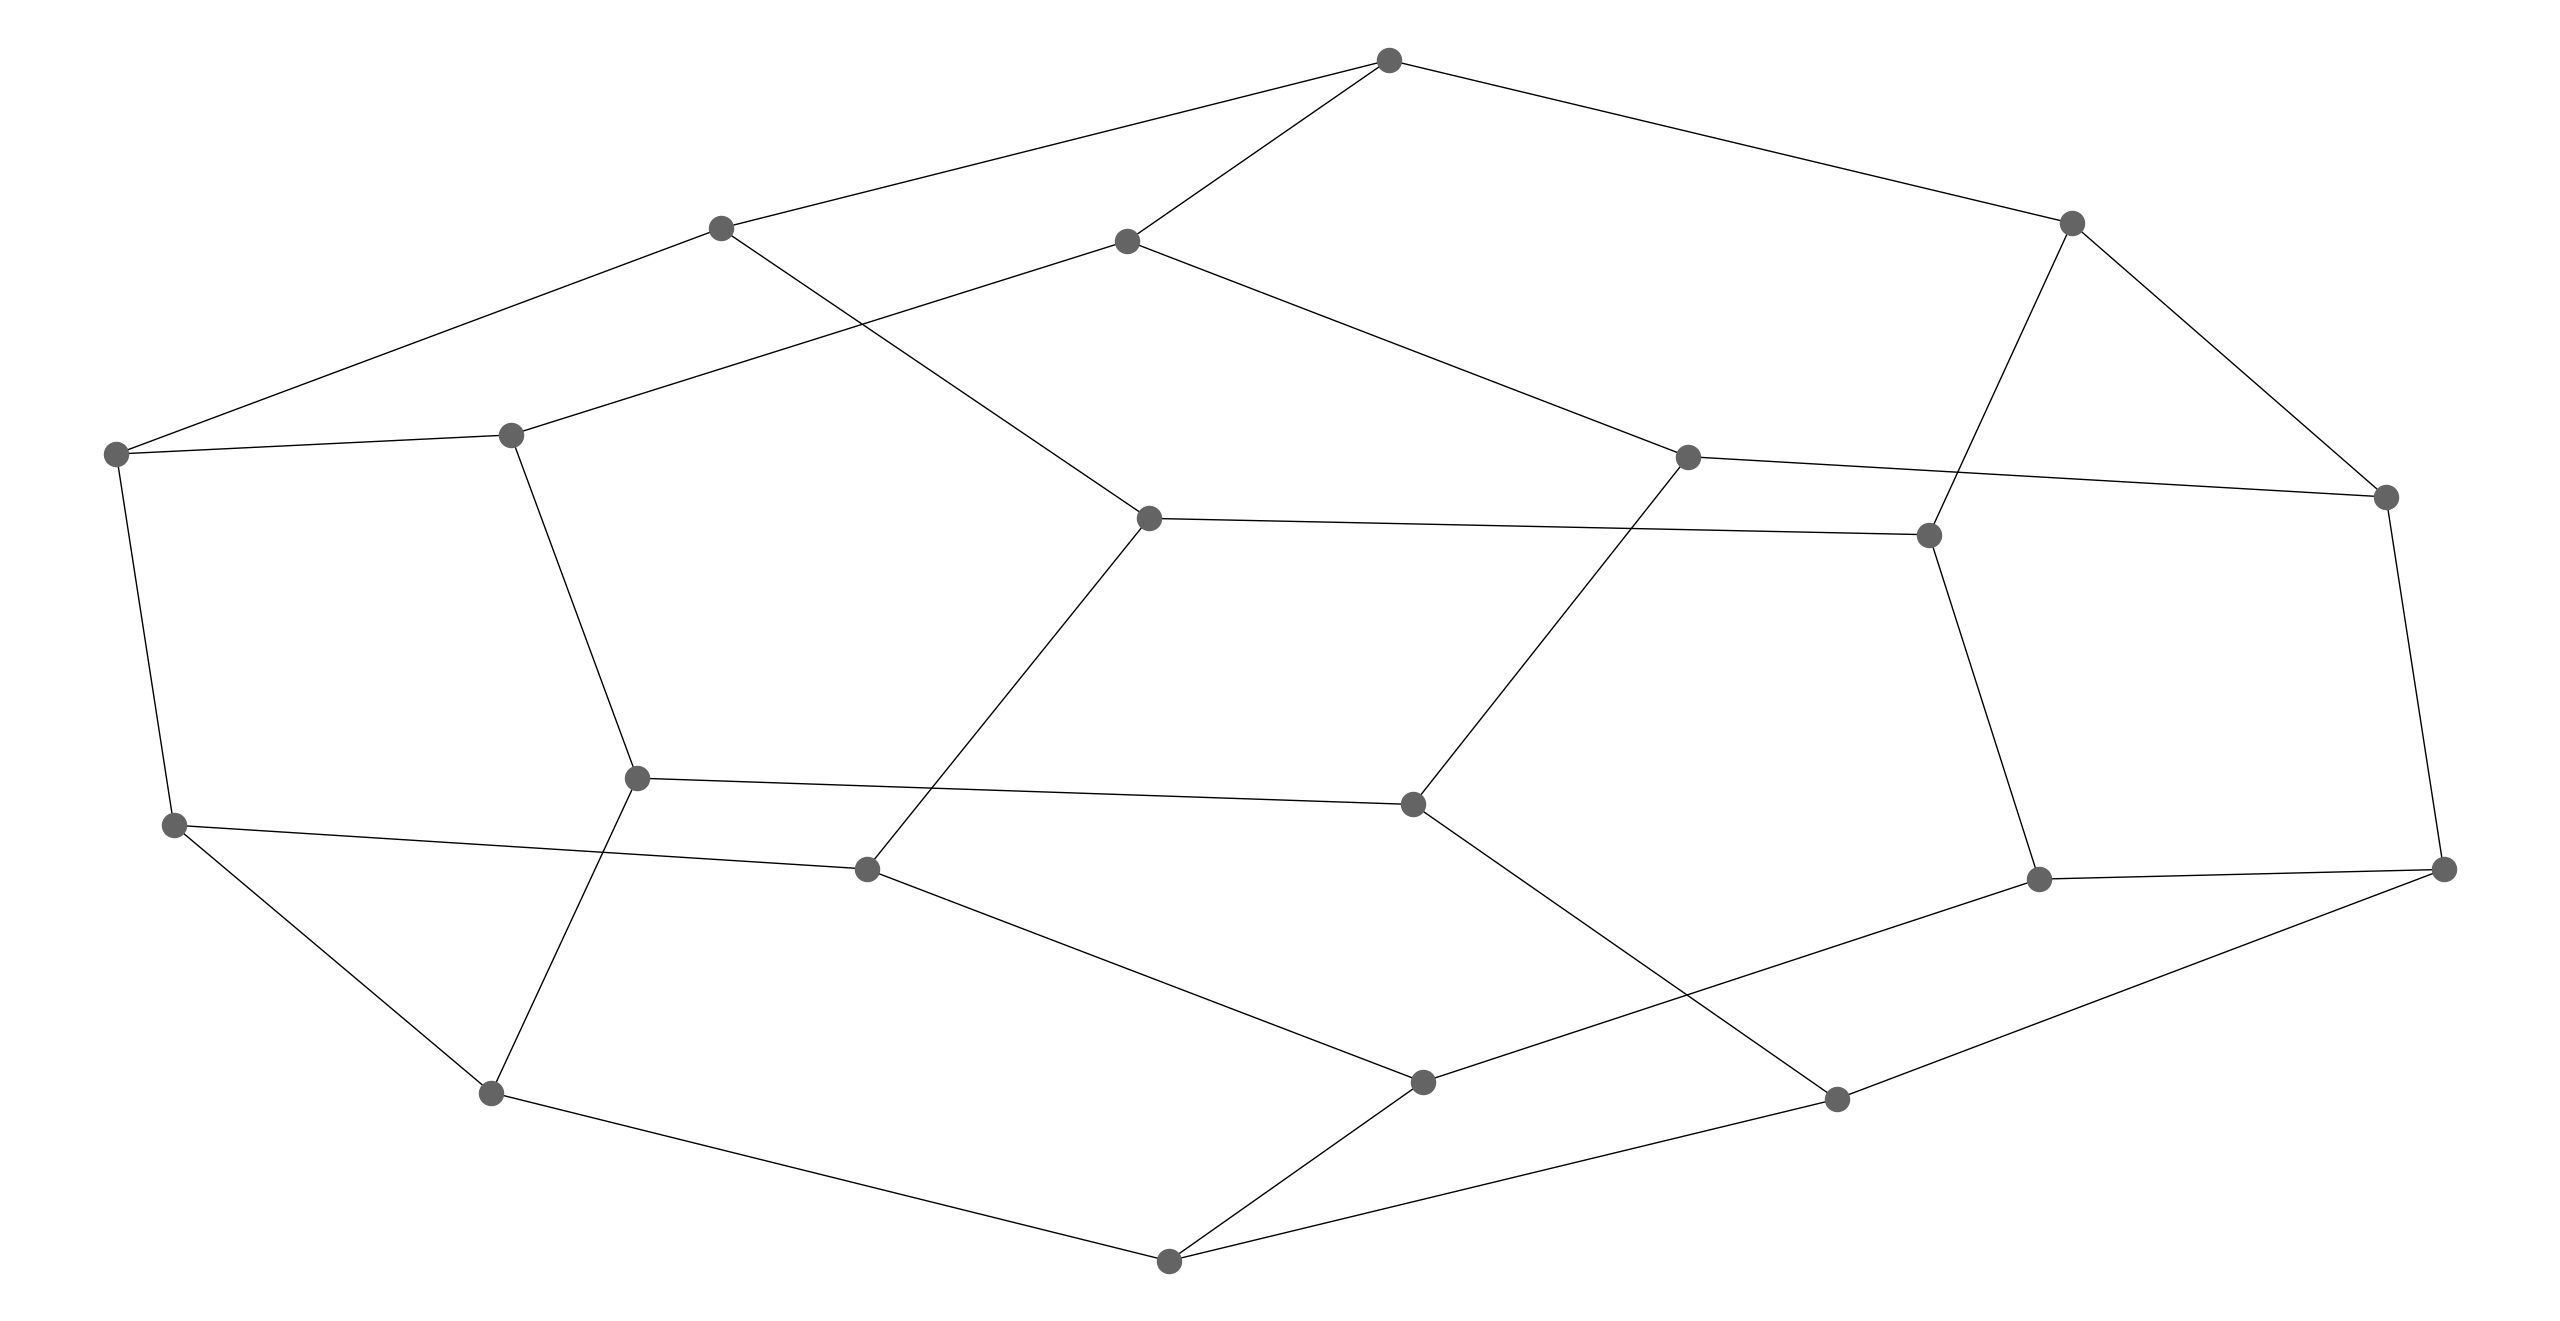
\includegraphics[height=100px]{simple_graph}
	\caption{Egyszerű gráf képi ábrázolása}
\end{figure}

Gyakorlatban különösen fontos tulajdonságnak bizonyult -- a könnyű értelmezhetőség szempontjából --, hogy egy adott gráf ábrázolható-e anélkül, hogy bármely két éle metszené egymást, azaz \textit{síkbarajzolható-e}. A gráfelmélet egy ismert tétele, hogy nem minden gráf rajzolható síkba. A \textbf{Fáry-Wagner} tétel továbbá kimondja, hogy minden olyan gráf, ami görbe vonalak használatával síkbarajzolható, az egyenes vonalak esetén is az marad.

Annak ellenére, hogy a reprezentáció aránylag egységes, rengeteg módszer létezik a konkrét csúcselrendezési feladat megoldására (ami természetesen implikál egy teljes gráfkirajzolást is). Ezen módszerek aztán csoportosíthatók, így ismerünk egyszerű konstruktív szabályokon (például köríven vagy rácson való elhelyezésen) alapulókat\cite{graph_layout_circular, graph_layout_circular2, graph_layout_orthogonal}, a Laplace-mátrix sajátvektorait használó spektrális elrendezéseket\cite{graph_layout_spectral} és -- jellemzően -- rúgóként kezelt élek és elektronokként tekintett csúcsok egyensúlyi állapotát kereső erőalapú (force-directed) módszereket\cite{graph_layout_force_directed, graph_layout_force_directed2}. A mi szempontunkból ezutóbbi lesz a legfontosabb, azon belül is Fruchterman és Reingold megoldása\cite{graph_layout_fruchterman}. Természetesen a korábbiak nem mindig különülnek el teljesen, előfordul, hogy több kategóriába is sorolható egyazon algoritmus\cite{graph_layout_hybrid}.

\subsection{Hipergráfok és halmazrendszerek ábrázolása}

Gráfokhoz hasonlóan hipergráfok (és/vagy halmazrendszerek) esetén is hasznos a felhasználó által értelmezhető ábrázolásuk, azonban -- a gráfoktól eltérő módon -- a vizuális reprezentációjuk már egyáltalán nem egységes. A szakirodalom számos különböző módszert tart nyilván, melyeket Alsallakh és társai foglaltak össze\cite{alsallakah2016_the_state_of_the_art_set_visualization}. Ugyan Alsallakhék számos kategóriába sorolták a módszereket, azonban -- véleményem szerint -- kis variációk is könnyen összemossák az ezek közti határokat. Bár én általánosabb kategóriák szerint tekintem át a módszereket, ezek sem tekinthetők abszolútnak, gyakori a hibridek használata.

A legtöbb cikk régióalapú módszereket alkalmaz, ahol az egyes halmazok és egymáshoz való viszonyuk a sík részterületeivel vannak reprezentálva, míg a régiók elkülönítése jellemzően színkódolással történik\cite{eulerape, euler_polygon_article, simonetto_undrawable} (az ebben a fejezetben bevezetett Euler-diagramok is ebbe a kategóriába tartoznak). Egy másik népszerű eszköz a gráfszerű leírás. Ide tartozik például a halmazok görbevonalként való leírása, amelyek akkor tartalmaznak egy csúcsot, ha átmennek azon\cite{linesets}. Elképzelhető továbbá a szuperduális használata is, amely végső soron tökéletesen reprezentál egy hipergráfot, azonban a tartalmazás reláció nehezebben felismerhető válik tőle. A bipartite incidence structure használata esetén ez a probléma már nem merül fel, viszont Skiena kivételével -- aki mindössze megemlíti az alkalmazhatóságát\cite{bpis_vis} -- nem találtam olyan cikket, amely közvetlenül használná. Természetesen mátrixokkal (pl. incidencia mátrix segítségével) is ábrázolható egy hipergráf. Különböző aggregációt használó algoritmusok is előfordulnak, amelyek leginkább méretarányos diagramok vagy felhasználói interakció bevezetésével operálnak\cite{wellmatched_important, interactive_sets}, habár ezek nem különösöbben elterjedtek. Ennek ellenére Chapmanék empirikus értékelése szerint az általuk használt aggregációs módszer könnyebben és jobban értelmezhető volt, mint a népszerűbb, Euler-diagramokon alapuló megoldások\cite{wellmatched_important}. Előfordul továbbá, hogy információt ikonokkal írnak le, speciálisan a régióalapú megoldásoknál glyphnek nevezzük, mikor az egyes metszetek fölötti ikon(ok) méretével vagy számával jelezzük azok elemeinek számát.

%Az említett cikk az ábrázolási módok számos kategóriáját különbözteti meg. Én ezek közül kiemelném, hogy léteznek gráfokon, régiókon, vonalakon, mátrixokon és aggregáción alapuló, illetve hibrid módszerek. Az egyes kategóriák önmagukban is több ábrázolási módszert fednek, melyeket jellemzően egyenként is szakcikkek sokasága fed, így az áttekintésükre itt nincs módunk, azonban jól mutatja a kutatási terület mélységét.


Ebben a dolgozatban egy specifikus, régióalapú ábrázolási mód, az Euler-diagram vizsgálatát tűztem ki célul. Az Euler-diagram kirajzolását célzó algoritmusok az úgynevezett Euler Diagram Generation Problem (EDGP) megoldásai. Ahogy a neve is mutatja, a szóban forgó ábrázolási módot még maga Leonhard Euler vezette be a XVIII. században, azonban mindmáig előszeretettel használatos. Ahogy Baron írja\cite{euler_early}, Euler mindössze példákon mutatta be, illetve alkalmazta módszerét, nem definálta explicit módon. Ezek alapján -- a hipergráfokhoz mintájára -- Euler-diagramokra is többféle definíció létezik, melyek mind megyeznek abban, hogy az egyes halmazok/hiperélek zárt görbékkel reprezentáltak, melyek metszetei közös halmazelemeket feltételeznek, míg diszjunkt esetben azok hiányát. Egyes definíciók az alaphalmaz elemeit/hipercsúcsokat is elhelyezik az ábrán, így létrejöhetnek olyan metszetek is a vizualizáció során, melyek valójából üresek, de az értelmezés során -- elviekben -- ez mégsem okoz gondot. Más esetekben üres részhalmazok létrejötte nem engedélyezett vagy egy speciális színnel jelölendő. Gyakori kérdés, hogy a zárt görbék körök, ellipszisek vagy tetszőleges formájúak lehetnek-e, hogy szükségszerűen konvexek-e, illetve az egyes halmazok több, azonos címkével ellátott görbével is reprezentálhatók-e. A következőkben definiálom, hogy ebben a dolgozatban milyen értelmezést használok, azonban -- az előzőeknek megfelelően -- egyéb források ettől eltérhetnek.

\begin{definition}
A továbbiakban a $H=(V,E)$ hipergráfot reprezentáló \textbf{egyszerű Euler-diagram} alatt egy olyan ábrát értünk, amelyben minden $e \in E$ halmaz egyetlen zárt görbére képződik le, mely azokat, és csak azokat a hipercsúcsokat tartalmazza, melyek az adott $e$ hiperélnek is elemei. Azon hipercsúcsok, melyek egyetlen hiperélben sem szerepelnek, az összes görbén kívül kell megjelenjenek. Az egyes görbék címkével (esetünkben színekkel) rendelkeznek.
\end{definition}

\begin{figure}[H]
	\centering
	\subfigure[Ellipszisalapú Euler-diagram\cite{eulerape}]{
		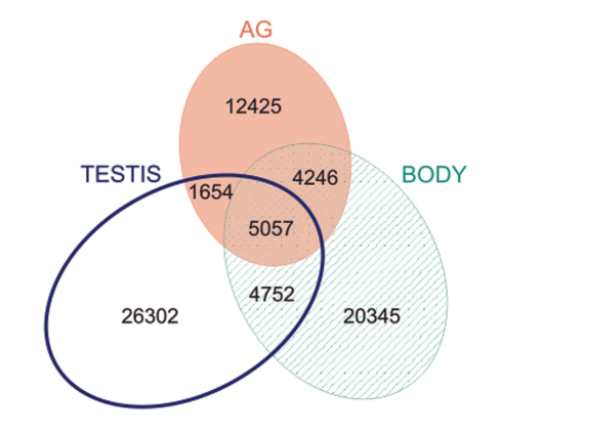
\includegraphics[width=0.45\linewidth]{euler_ellipse}}
	\hspace{5pt}
	\subfigure[Poligonalapú Euler-diagram\cite{euler_polygon_article}]{
		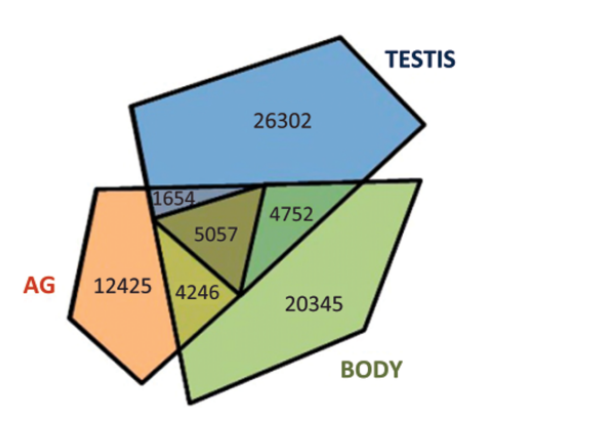
\includegraphics[width=0.45\linewidth]{euler_polygon}}
	\caption{Egyszerű Euler-diagramok}
	\label{fig:euler_simple}
\end{figure}

\begin{definition}
\textbf{Általánosított Euler-diagramként} fogom nevezni azt az egyszerű Euler-diagramot, mely egy hiperélt több, azonos címkével ellátott zárt görbére is leképezhet.
\end{definition}

\begin{figure}[H]
	\centering
	\subfigure[Általánosított Euler-diagram\cite{simonetto_undrawable}]{
		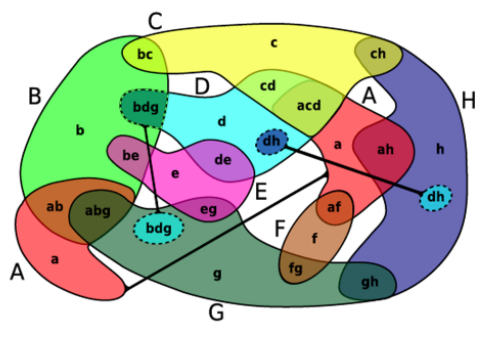
\includegraphics[width=0.45\linewidth]{euler_general}}
	\hspace{5pt}
	\subfigure[Hibrid Euler-diagram glyphekkel\cite{euler_glyph_article}]{
		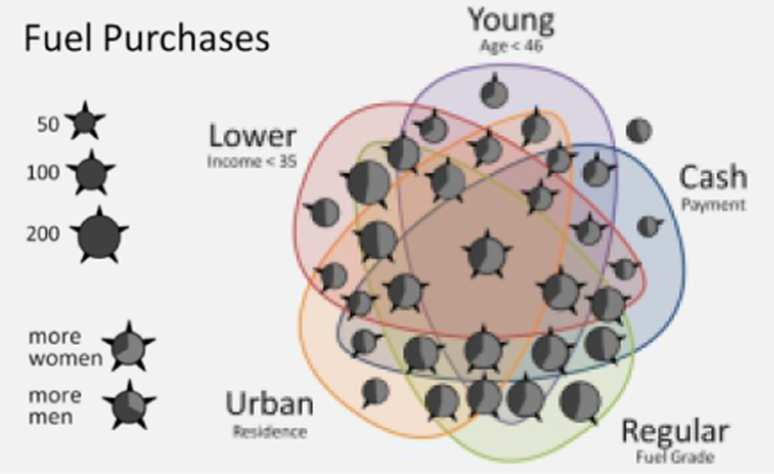
\includegraphics[width=0.45\linewidth]{euler_glyph}}
	\caption{Euler-diagram variánsok}
	\label{fig:euler_general}
\end{figure}



\subsection{Euler-diagramok vizualizációja}

\subsubsection{Síkbarajzolhatóság}
Gráfok esetében láthattuk, hogy felmerül a síkbarajzolhatóság kérdése. Egy hipergráf akkor síkbarajzolható, ha a kirajzolása során nem jön létre olyan régió, amely üres halmazt reprezentál. Amennyiben egyszer Euler-diagramokkal, így zárt, a végpontokat (jelen esetben hipercsúcsokat) tartalmazó görbékkel reprezentáljuk az éleket, akkor rögtön láthatjuk, hogy ezeknek tartalmazniuk kell legalább egy görbét is, amely közvetlenül összeköti a végpontokat. Ebből már észrevehetjük, hogy csúcsok használata nélkül nem minden hipergráf rajzolható síkba egyszerű Euler-diagramokkal.


Verroust és Viaud bebizonyította\cite{drawability_8_sets}, hogy az általuk használt Euler-diagram definíció 8 halmazig megőrzi a síkbarajzolhatósági tulajdonságot. Simonetto és Auber egy másik struktúrát vizsgált\cite{simonetto_undrawable}, ami megfelel az itt általánosított Euler-diagramként definiált fogalomnak (ők Euler representationnek nevezik), melyről levezették, hogy alkalmas tetszőleges hipergráf síkbarajzolására, görbéknek kizárólag szemantikailag helyes metszeteinek létrehozása mellett (akár csúcsok használata nélkül is). A szuperduális felhasználásával pontos leírása is adható annak, hogy mikor nem rajzolható ki egy hipergráf egyszerű Euler-diagramok használatával\cite{simonetto_undrawable, drawability_8_sets}. (Megjegyzendő, hogy a Simonetto cikk intersection graphnak nevezi a szuperduálist, miközben az egy másik struktúrát jelöl, de a leírásból, illetve a példákból levezethető, hogy valójából felcserélték a kettőt.)

\subsubsection{Esztétikai mértékek} \label{eulerAesthetic}

Természetesen egy diagram nem csak a mögöttes struktúra (halmazrendszer vagy hipergráf) leképezéséhez feltétlenül szükséges szemantikai tulajdonságokkal bírhat. Egy adott ábrának az emberi értelmezést segítő tulajdonságait esztétikai vagy ergonómiai tulajdonságoknak nevezzük, ha pedig számszerűsíthetők (és adott rajtuk egy teljes rendezés), akkor esztétikai metrikáknak hívjuk. Esztétikai metrikák definiálhatók magukon a görbéken, a görbék metszetein, a csúcsok eloszlásán, az ábra színezésén, továbbá -- gyakorlatilag -- az ábrán megjelenő bármely egyéb aspektus fölött \cite{euler_force, which_well_formed, layout_metrics}.


Az EDGP során felmerülő két leggyakrabban vizsgált\cite{wellmatched_important, euler_force, which_well_formed, well_matchedness, orientation_comprehension} esztétikai tulajdonság, az úgynevezett well-formed és well-matched tulajdonságok.

\begin{definition}
Egy adott Euler-diagram esetén \textbf{kontúr/contour} névvel illetjük az egy címkéhez (vagy hiperélhez/halmazhoz) tartozó különböző zárt görbék összességét. \textbf{Minimális régiónak/minimal regionnek} hívjuk a görbék és metszeteik által létrehozott legkisebb síkpartíciókat, míg \textbf{alaprégió/basic region} alatt azon minimális régiók halmazát értjük, melyek ugyanazon görbék részei. Egy \textbf{zóna/zone} az alaprégiók egy olyan halmaza, amelyeket azonos címkével rendelkező görbék tartalmaznak.
\end{definition}

A well-formed tulajdonság hat kritériumból tevődik össze, bár néha csak az első ötöt használják:

\begin{compactenum} \label{wfc}
	\item Minden görbe egyszerű, azaz nem metszi önmagát. - WFC1 \label{step:wfc1}
	\item Nincs két görbe, amelynek közös határolószakasza van. (Az elfajuló, pontbeli találkozást nem vesszük hozzá.) - WFC2 \label{step:wfc2}
	\item Nincs olyan pont, ahol három görbe érintkezik. - WFC3 \label{step:wfc3}
	\item Ha két görbe érintkezik, akkor metszik egymást. - WFC4 \label{step:wfc4}
	\item Minden zóna összefüggő, azaz egyetlen minimális régióból áll. - WFC5 \label{step:wfc5}
	\item Nem rendelkezik két görbe azonos címkével. - WFC6 \label{step:wfc6}\\
\end{compactenum}

Egy Euler-diagram well-matched, ha a zónák, görbék, minimális régiók és kontúrok szintjén is az. A különböző esetekben ezek az alábbiakat fedik:

\begin{compactenum}
	\item Zónák szintjén: nem tartalmaz üres zónákat. - WMP1
	\item Görbék szintjén: a halmazok közti részhalmaz, metszet és diszjunkció relációk megfelelnek az adott halmazokat reprezentáló görbék tartalmazás, átfedés és diszjunkció tulajdonságának. - WMP2
	\item Minimális régiók szintjén: well-matched a zónák szintjén, és csak összefüggő zónákat tartalmaz. - WMP3
	\item Kontúrok szintjén: a halmazok közti részhalmaz, metszet és diszjunkció relációk megfelelnek az adott halmazokat reprezentáló kontúrok tartalmazás, átfedés és diszjunkció tulajdonságának. - WMP4
\end{compactenum}

Szintúgy széles körben vizsgált tulajdonság az area-proportionality, avagy méretarányosság\cite{euler_with_circles, area_proportional_phd, drawing_area_proportional, general_area_proportional}, amely azt mondja ki, hogy minden régió (bizonyos definíciók szerint az univerzumot reprezentáló kivételével) mérete úgy aránylik az ilyenek összegéhez, mint az $\omega$ súlyfüggvényük azok összegéhez. Leggyakrabban a régió által tartalmazott elemek számát alkalmazzuk súlyfüggvényként. Hibamértékek segítségével könnyen metrika is előállítható a tulajdonságból.


Egyes szerzők a régiók színezését is hasonlóan fontosnak ismerik el, mint az elhelyezkedésüket\cite{imdb_euler, how_color_euler}.


Annak ellenére, hogy több esztétikai metrika és tulajdonság is széles körben alkalmazott, nagyon kevés empirikus tapasztalatunk van arról, hogy ezek ténylegesen befolyásolják-e egy ábra értelmezhetőségét. Fish és társai kis mintán vizsgálták\cite{euler_comprehension} a well-formed tulajdonságnak az ábrák megértésére vonatkozó hatását. Az ő eredményeik alapján a WFC2 megsértése akár segítheti is egy ábra értelmezését, míg a WFC1 és WFC4 egyidejű, illetve a WFC3 vagy WFC4 önálló megsértése is rontja azt. Blake és társai\cite{orientation_comprehension} arra az eredményre jutottak, hogy az egyes görbék orientációja nincs hatással az emberi percepciójukra. Blake-ék, egy másik cikkükben\cite{shape_comprehension}, a szimmetrikus alakzatokat azonosították a legkönnyebben megérthetőként, így különösen a kör alakú reprezentációt javasolják. Chapman és társai empirikus módon arra az eredményre jutottak\cite{wellmatched_important}, hogy a well-matched tulajdonság fontosabb, mint a well-formed.

\subsubsection{Euler-diagramok generálása}

Még úgy is, hogy az Euler-diagramok mindössze részterületét képezik a halmazábrázolási módszereknek, a szakirodalomban rengeteg különböző eljárás található, melyek gyakran nem is tekinthetők ugyanannak a szűken vett probléma megoldásának. Az alkalmazott Euler-diagram definíció, a vizsgált probléma mérete, az alkalmazott esztétikai tulajdonságok és metrikák, illetve ezek erős vagy gyenge megkövetelése mind-mind új variánsait hozzák létre a -- összefoglaló néven EDGP-nek nevezett -- problémának.

A -- már említett -- Allsalakh cikk\cite{alsallakah2016_the_state_of_the_art_set_visualization} nem kizárólag a szakirodalomban előforduló EDGP módszereket mutatja be, de ezeket különböző szempontok szerint össze is hasonlítja. Elsősorban megkülönbözteti a tetszőleges relációk ábrázolására alkalmas, illetve az ebben a tekintetben korlátozott megoldásokat. Ettől nem függetlenül megadják, hogy milyen alakzatokkal reprezentál egy halmazt az adott módszer (kör, poligon vagy ellipszis), a cikkből azonban sajnos kimaradt, hogy ismert Bézier-görbe alapú megoldás is\cite{layout_metrics}. Másik szempontként hozzák fel a teljesített esztétikai tulajdonságokat, mint a well-formed, well-matched, area-proportional, szimmetrikus görbe tulajdonságokat, és vizsgálják, hogy létrejönnek-e üres minimális régiók (az univerzumon kívül). Az általuk adott összehasonlítás alapján továbbá azt tételezhetjük fel, hogy az egyes módszerek vagy három, vagy tetszőleges számú halmazra alkalmazhatók. Megfigyelhető, hogy ezutóbbi az alapján válik el, hogy az Euler-diagramok egy speciális esetét, a Venn-diagramokat vizsgálja-e egy adott cikk vagy az általános problémát. Amiről ezek alapján nem kapunk képet, hogy egyes módszerek csak 8 halmazig alkalmazhatók\cite{drawability_8_sets}, mivel ezek fölött már ismertek olyan példák\cite{simonetto_undrawable, drawability_8_sets, inductive_euler}, amelyek nem síkbarajzolhatók egyes Euler-diagram definíciók szerint. (A cikkben nem említett, de hasznos kiemelni, hogy egyes algoritmusok csak már meglévő diagramok esztétikai javítását szolgálják\cite{euler_force} vagy emberi beavatkozást igényelnek\cite{sketch_euler}.)

A dolgozat későbbi részeiben legfontosabbnak Flower, Rodgers és Mutton munkája\cite{layout_metrics} fog bizonyulni, akik sztochasztikus optimalizációs módszereket, illetve metaheurisztikákat alkalmaztak Bézier-görbékkel reprezentált Euler-diagramokra, és akikkel részben hasonló megközelítést választottunk. Érdemes még megemlíteni Stapleton és társainak munkáját\cite{inductive_euler}, amelyben induktív módon generálnak well-formed euler diagramokat, mikor ez lehetséges, a többi esetben pedig a well-formed kritériumok megsértésével, a görbék önmetszésével érik el, hogy továbbra is szemantikailag helyes ábrát generáljanak. Különösen érdemes megfigyelni, hogy az általánosság ilyen szintű eléréséhez a duális gráf egy módosított verzióját használják, ami exponenciális futásidőt eredményez.

\subsection{Problémaleírás}

Láthattuk, hogy az EDGP egy összetett probléma, amely magában foglalja a konkrét ábrázolási mód (Euler-diagram definíció), a vizsgált esztétikai metrikák, az elfogadható futásidő és a megoldható problémaméret meghatározását is. Különösen fontos kitérni arra is, hogy egy adott probléma vizsgálata során nem feltétlenül egyféle szempont szeretnénk ábrázolási módot választani, elképzelhető például, hogy ugyanúgy szeretnénk az előforduló klasztereket vizsgálni, mint a leghosszabb utakat, melyek másféle elrendezést tételeznek fel.

Ebben a dolgozatban az abszolút általános EDGP megoldás felé igyekszem egy lépést tenni, amennyiben -- direkt módszerekkel szemben  -- többféle esztétikai metrika kezelésére is képes optimalizációs módszerek alkalmazhatóságát vizsgálom általánosított Euler-diagramok esetén. A szakirodalomnak megfelelően egy-két tucat hiperélig és legfeljebb száz csúcsig vizsgálom a problémát. Mivel ez egy kísérletsorozat, ezért a futásidőre megkötést nem teszek, azonban az eljárások kidolgozása során probléma méretében exponenciális futásidejű megoldásokat kizárom.

%A tématerület bonyolultságának és mélységének megfelelően a dolgozat különböző módszerek vizsgálatáról szól, a végső eszközt még nem hivatott létrehozni.
Különösképp megnehezíti a feladatot az általános megoldás igénye, illetve Alsallakhék (a halmazábrázolási módszereket áttekintő cikkükben\cite{alsallakah2016_the_state_of_the_art_set_visualization} tett) megállapítása, miszerint az Euler-diagramok mindössze 10-20 halmazig alkalmazhatók.


Mint láthattuk, az általános megoldhatóság érdekében emberi beavatkozás, korlát nélküli paramétertér (például Bézier görbék kontrollpontjai\cite{layout_metrics}) vagy exponenciális futásidő\cite{inductive_euler} lehet szükséges. Mivel tetszőleges esztétikai metrika fölött az optimalizáció, így a legjobb Euler-diagram megtalálása is NP-nehéz, ezért ez egyáltalán nem meglepő. A megoldásom alapjaként választott Flower cikkel\cite{layout_metrics} szemben, az általam használt, bonyolultabb problématér (mind a hipergráf méretében, egy adott halmazt reprezentáló zárt görbék számában és ebből kifolyólag a költségfüggvényként alkalmazott heurisztikák nem-folytonos jellegében) felveti a diagram modell egyszerűsítésének igényét, illetve újabb heurisztikák kidolgozásának szükségességét.


Vizsgálataimat ezért megelőzi egy diagram modell, a rászabott -- de a szakirodalmi megállapításokon alapuló -- heurisztikák és az optimalizációs algoritmusok egyedi variánsainak kialakítása.

% -------------------------------------------------------------------------------------

\section{Megoldás}

\subsection{Optimalizáció} \label{optimization}

A matematikai optimalizáció célja egy adott $f: X \rightarrow \mathbb{R} $ valós értékű függvény globális minimum- vagy maximumhelyének megtalálása, ahol X tetszőleges halmaz lehet. Mivel az $f$ függvény negáltja segítségével maximalizációs problémák minimalizáliós problémákká vezethetők vissza (vagy fordítva), ezért a kettő feladatot azonosnak tekintjük. A továbbiakban -- mikor nem jelzem az ellenkezőjét -- minimalizálási problémát tételezek fel.

\begin{definition}
Az $f$ függvényt számos módon nevezik; minimalizálási problémák esetén \textbf{költség-/veszteségfüggvényként} vagy \textbf{objektívfüggvényként}, míg maximálizálási problémák esetében \textbf{utility} vagy \textbf{fitness functionként} ismerjük. Egyes szakterületeken (mint fizikában) egyéb nevek is ismertek. Ha az $f$ függvény a $g_i, i \in \mathbb{N}_0$ függvények átlagaként áll elő, akkor költségfüggvénynek hívjuk, a $g_i$ függvényeket pedig veszteségfüggvényeknek.
\end{definition}

\begin{definition}
Egy optimalizálási algoritmus paramétereit \textbf{hiperparamétereknek} nevezzük.
\end{definition}

Általánosságban beszélve az optimalizálási probléma NP-nehéz, azonban a költségfüggvényre tett megszorításokkal ez feloldható. Különösen fontos ezért, hogy az egyes algoritmusok, hogy milyen megszorítások mellett operálnak.

\subsubsection{Gradiensalapú optimalizáció}
Gradiens-, illetve deriváltalapú algoritmusok vagy a deriváltfüggvényt (Hesse-mátrixot) vagy a pontbeli (parciális) deriváltat alkalmazzák. Bár szigorúan véve az első- és másodikderivált-próba is ide tartozik, a gyakorlatban a vizsgált függvény pontos képlete jellemzően nem ismert, illetve a paraméterek és a lokális szélsőértékek nagy száma is ellehetetleníti ezt a féle megoldást. Ezzel szemben iteratív mószereket szokás használni, melyek egy megadott -- általában véletlenszerű -- kiindulópontból egy lokális minimumponthoz konvergálnak. Amennyiben a függvény konvex vagy a kiindulópont kellőképpen közel volt a globális minimumhoz, akkor a kapott lokális minimumhely globálisan is az lesz, azonban ez általában nem garantált. Az előzőeknek megfelelően sokszor elvárt tulajdonság a folytonos deriválhatóság is.


A gyakorlatban használt legtöbb iteratív algoritmus a gradiens leszálláson alapszik. Gradiens leszállás során egy tetszőleges $\theta_0$ kiindulópontot választunk, majd a $\theta_{i+1} = \theta_i - \alpha * \nabla f(\theta_i)$ szabály alapján kiválasztjuk a következő vizsgálandó pontot, ahol $\alpha$ egy hiperparaméter. Az iteráció addig folytatódik, míg a megállási feltétel (például felső korlát az iterációk számára, a lépésköz nagyságára vagy a gradiens egy normájára) nem teljesül. Fontos tulajdonsága ennek az algoritmusnak, hogy túl nagynak megválasztva $\alpha$-t átugorhatunk minimumhelyeket, míg túl kicsire állításával a keresési időt növeljük meg. Számos módszer született ennek a hiányosságnak az áthidalására, így egyes variációk az iterációk számának növekedésének függvényében csökkentik $\alpha$-t vagy eltérő kiindulópontokból indítják újra a keresést. Bizonyos feltételek mellett az algoritmus garantáltan egy lokális minimumhelyhez konvergál\cite{gradient_convergence}.


A gradiensalapú módszerekkel rokon jegyeket mutat a -- nem feltétlenül differenciálható, de konvex függvények esetében a alkalmazható -- szubgradiensmódszer, illetve az általánosabban használható, lokális keresésen alapuló hegymászó algoritmus.
% (hill climbing).

\subsubsection{Sztochasztikus algoritmusok}

Összefoglaló néven \textbf{sztochasztikus algoritmus} névvel illetjük azokat a módszereket, amelyek futásuk során valószínűségi változókat alkalmaznak. Ez a megközelítés gyakran használt, mikor a költségfüggvény nem alkalmas direkt optimalizációra, viszont megelégszünk közelítő megoldásokkal is. Szintúgy előnyös, mikor a keresési térben számos, globális minimumértékhez közel álló pont létezik. A gradiens leszállás során látott véletlen kezdőpont kiválasztását inputnak tekintjük, így az algoritmus alapverzióját nem tekintjük sztochasztikusnak, viszont -- mint számos egyéb determinisztikus (nem sztochasztikus) algoritmusnak -- vannak sztochasztikus variánsai. Ennek megfelelően fontos kiemelni, hogy az egyes optimalizációs módszereknek általában több variánsa is létezhet, melyek esetenként összemossák a kategóriákat. Ennek a fejezetnek a további részében át fogjuk tekinteni azokat az algoritmusokat, amelyeknek szükséges az ismerete a továbbiakban, azonban néhol pont az itt bemutatott alapverziótól való eltérés lesz különösen érdekes.


A legismertebb ilyen variáns az úgynevezett \textbf{sztochasztikus gradiens leszállás} (SGD). Mikor az $f$ költségfüggvény több $f_i$ veszteségfüggvény átlagaként jön létre, azaz $f(x) = 1/n * \sum_{i=1}^{n} f_i(x)$ (például gépi tanulás során több mintaelemen alkalmazva ugyanazt a veszteségfüggvényt), akkor előfordul, hogy a gradiens leszállás során a mai számítógépek kapacitásához képest túl sok parciális deriváltat kéne kiértékelni. Az SGD ezt úgy kerüli el, hogy a veszteségfüggvényeket egyesével értekeli ki, mindegyik kiértékelés után modósítva a paramétereket. Láthatóan ez nem ekvivalens a teljes költségfüggvény gradiensének használatával (csak közelíti azt), továbbá nagyban függ a kiértékelés sorrendjétől is, ezért a veszteségfüggvények sorrendje a kiértékelés során randomizált. Néha szintúgy SGD-nek nevezik a mini-batch gradient descent módszert, ami annyiban tér el az SGD-től, hogy a paraméterek módosítása során egyszerre $k$ darab veszteségfüggvény átlagát használjuk, ahol $k$ egy hiperparaméter.


Természetben lejátszódó folyamatok számos esetben optimalizációs módszerként is tekinthetők. A természeti megfigyelésekből adaptált optimalizációs technikákat összefoglaló néven \textbf{biologiailag inspirált} algoritmusoknak nevezzük. A természeti rendszerek komplexitásából fakadó modellezési bizonytalanság feloldását sokszor a sztochaszticitás bevezetésével érjük el, így -- gyakorlatban -- a legtöbb biológiailag inspirált optimalizációs algoritmus egyben sztochasztikus algoritmus is.


Egy ilyen, természet ihlette algoritmus, a természetes szelekción alapuló \textbf{genetikus algoritmus} (GA)\cite{genetic_algorithm, non_gradient_optimization}. A módszer mögötti megfontolás, hogy egy populáció életciklusa a új egyedek születéséből/halálából, az egyedek szaporodásából (így genetikai keveredéséből), illetve mutációkból tevődik össze, ahol a párosodás a gének előnyös jellegének $f$-nek függvénye. Az algoritmus célja, hogy ezt az $f$ fitness függvényt \textit{maximalizálja}, az életképes egyedek kombinációjával, illetve kis perturbációkkal.
%, véletlenszerű módosításokkal.
%Az algoritmus pszeudokódja alább látható, azonban nem térünk ki minden részletére.

\begin{algorithm}[H]
\caption{Genetikus algoritmus (saját szerkesztés)}
\label{alg:ga} 
\textbf{\underline{Function}} GA($populationSize, selectionRate, mutationRate$)
\begin{algorithmic}[1] % sorszámok megjelenítése minden n. sor előtt, most n = 1
\STATE $t = 0$
\STATE $population_t$ = generateFeasibleSolutions($populationSize$)
\STATE $values$ = evaluateFitness($population_t$)
\STATE $bestFitness, bestPosition = updateBest(values, \infty, population_t, bestPosition)$
\algstore{ga}
\end{algorithmic}
\end{algorithm}

\begin{algorithm}[H]
\begin{algorithmic}[1] % sorszámok megjelenítése minden n. sor előtt, most n = 1
\algrestore{ga}
\WHILE{megállási feltétel nem teljesült}
	\STATE $parents$ = selectFitnessProportionally($population_t, values, selectionRate$)
	\STATE $children$ = recombine($parents$)
	\STATE $population_t$ = deleteLast($population_t, values, |children|$)
	\STATE $population_{t+1} = population_t \cup children$
	\STATE $population_{t+1}$ = mutate($population_{t+1}, mutationRate$)
	\STATE $values$ = evaluateFitness($population_{t+1}$)
	\STATE $bestFitness = updateBest(values, bestFitness, population_{t+1}, bestPosition)$
	\STATE $t = t + 1$
\ENDWHILE
\STATE \textbf{return} $bestFitness, bestPosition$
\end{algorithmic}
\end{algorithm}


Itt a $generateFeasibleSolutions(n)$ $n$ darab megengedett megoldást generál, $evaluateFitness(population)$ kiértékeli az egyes egyedek fitness értékeit, $updateBest(newValues, oldBest, newPositions, oldPosition)$ az új értékek és pozíciók, illetve a korábbi legjobbak segítségével kiválasztja a legjobbat (maximumot és maximumhelyet), $selectFitnessProportionally(population, fitnessValues, num)$ a fitness értékek által implikált valószínűségi eloszlás szerint kiválaszt $num$ darab egyedet, $recombine(population)$ két elemenként egy új egyedet hoz létre, amely a szülei génállományán alapszik, $deleteLast(population, fitnessValues, num)$ törli a $num$ darab legrosszabb fitness értékkel bíró egyedet a populációból, $mutate(population, mutationRate)$ pedig a $mutationRate$ arányában megváltoztatja az egyedek génállományát. A megállási feltétel gyakran iterációs felső korlát vagy alsó korlát a legjobb fitness értékre.


A \textbf{particle swarm optimization} (PSO) egy másik biológiailag inspirált algoritmus, amely analóg módon működik egyes rajként együtt dolgozó állat- és rovarfajokkal\cite{non_gradient_optimization, pso, modified_pso}. A módszer alapelve, hogy különböző, részecskéknek nevezett, entitások pozícióiban értékeljük ki az $f$ költségfüggvényt. A részecskék haladási iránnyal és sebességgel rendelkeznek, amelyet minden iterációban úgy frissítünk, hogy - véletlenszerű mértékben - figyelembe vesszük magát az irányt/sebességet és a részecske által, illetve a globálisan talált eddigi legjobb pozíciót/értéket.

%TODO check final page break

\begin{algorithm}[H]
\caption{Particle swarm optimization (Clerc alapján\cite{pso_alg})}
\label{alg:pso} 
\textbf{\underline{Function}} InitializePSO($S, lowerBounds, upperBounds, f$)
\begin{algorithmic}[1] % sorszámok megjelenítése minden n. sor előtt, most n = 1
\STATE $bestPosition_{global} = \emptyset$
\STATE $bestValue = \infty$
\STATE $bestValues[S] =$ empty array
\FOR{$i=1 \ldots S$}
	\STATE $bestPosition_i = particlePosition_i \sim U(lowerBounds, upperBounds)$
	\STATE $bestValues_i = f(bestPosition_i)$
	\STATE $velocityRange = |upperBounds-lowerBounds|$
	\STATE $velocity_i \sim U(-velocityRange, velocityRange)$
	\IF{$bestValues_i < bestValue$}
		\STATE $bestPosition_{global} = bestPosition_i$
		\STATE $bestValue = bestValues_i$
	\ENDIF
\ENDFOR
\WHILE{megállási feltétel nem teljesült}
	\FOR{$i=1 \ldots S$}
		\STATE $random_1, random_2 \sim U([0,1]^{dim(lowerBounds)})$
		\STATE $velocity_i = w*velocity_i + c_1*random_1*(bestPosition_i-particlePosition_i) + c_2*random_2*(bestPosition_{global}-particlePosition_i)$
		\STATE $particlePosition_i = particlePosition_i + velocity_i$ \COMMENT{néha $\ldots + \alpha * velocity_i$}
		\STATE $particleValue = f(particlePosition_i)$
		
		\IF{$particleValue < bestValues_i$}
			\STATE $bestPosition_i = particlePosition_i$
			\STATE $bestValues_i = particleValue$
			\IF{$bestValues_i < bestValue$}
				\STATE $bestPosition_{global} = bestPosition_i$
				\STATE $bestValue = bestValues_i$
			\ENDIF
		\ENDIF
	\ENDFOR
\ENDWHILE
\STATE \textbf{return} $bestValue, bestPosition_{global}$
\end{algorithmic}
\end{algorithm}


Ahogy látható algoritmus hiperparméterek segítségével adja meg a részecskék számát, illetve a módosítási szabály egyes tagjainak súlyát. % ez áttolható mögé, ha kell

\subsubsection{Egyéb optimalizációs módszerek}
Természetesen az áttekintett kategóriákat nem merítettük ki, számos további algoritmus és variáns áttekintésére a dolgozat keretei között nincsen lehetőségem, illetve további megszorítások és függvényosztályok is ismertek, amelyekre létezik optimalizációs algoritmus, mint például lineáris egyenlőtlenségrendszerek vagy diszkrét halmazok esetén.

\subsection{Függvényapproximáció}

A numerikus analízis -- így például az optimalizáció -- számos területén merül fel a -- jellemzően valós értékű -- matematikai függvények használatának az igénye. Mikor a vizsgált függvény túl komplex, nem mindenhol kiértékelhető, esetleg nem rendelkezik az elvárt tulajdonságokkal, akkor függvények egy meghatározott részhalmazából kiválaszthatunk egy az eredetire legjobban illeszkedőt. Ezt az eljárást -- mint az ezt vizsgáló szakterületet -- \textbf{függvényapproximációnak} nevezzük. Mikor meghatározott pontokban várjuk csak el a legjobb illeszkedést, akkor görbék illesztéséről beszélünk.


Legyen $f = \left(\begin{smallmatrix}f_1 & \ldots & f_n\end{smallmatrix}\right)^\top, w \in \mathcal{R}^n$, ahol $f_i, i=1 \ldots n$ tetszőleges függvény lehet. Ekkor az $f(x, w)$ \textbf{lineáris függvényapproximátornak} nevezzük, ha az lineáris súlyok $w$ vektorában (bár nem feltétlenül az az $x$ inputban), azaz $f(x,w) = w_1*f_1(x) + \ldots + w_n*f_n(x)$. Mikor az $f$ függvény nem teljesíti a linearitási feltételt, akkor \textbf{nemlineáris függvényapproximátorról} beszélünk.

\subsection{Mesterséges neurális hálók}

Az egyik legismertebb és legszélesebb körben alkalmazott nemlineáris függvényapproximátorok a \textbf{mesterséges neurális hálók} (artificial neural network - ANN). Hasonlóan a biológiailag inspirált algoritmusokhoz, ezek olyan számítási rendszerek, amelyek biológiai folyamatokat, speciálisan az emberi - illetve állati - agyban működő neuronokat, és azok működését modellezik. Egy ANN legkönnyebben irányított gráfként képzelhető el, amelyben \textbf{(mesterséges) neuronok} alkotják a valós számokkal címkézett csúcsokat, míg a köztük létező, súllyal rendelkező kapcsolatok (szinapszisok) az éleket. A csúcsok címkéjét \textbf{biasnek} hívjuk, az élekét \textbf{weightnek}. A weight és a bias értékek közösen adják ki a neurális hálózat paramétereit. Az így kapott gráf számítási rendszerként fogható fel, amennyiben az egyes csúcsok műveleteket reprezentálnak. A forráscsúcsoknak közvetlenül beadhatók a rendszer bemenetei, míg az összes többi csúcs egy újabb értéket számít ki, melyek a nyelő csúcsokban értelmezhetők végeredményként. A források kivételével az egyes csúcsok az $x_v=\sigma(w_n \cdot x_n +b_v)$ képlet alapján számítják ki az értéküket, ahol $x_v$ a $v$ csúcs új értéke (nem címkéje), $w_n$ a bemenő élek súlyainak (weight) vektora, $x_n$ ezen élek kiindulópontjainak értéke, $b_v$ a $v$ csúcs címkéje/biase, a $\sigma$ függvény pedig egy - jellemzően nemlineáris - aktiválási függvény.

\subsubsection{Architektúra}

A számítási gráf csúcsait általában a forrásoktól való távolságuk alapján szokás ún. \textbf{rétegekbe} particionálni, ahol strukturálisan az egyes rétegek általában minden csúcsukban azonos módon viselkednek. A rétegekre bontás számos előnyös tulajdonsághoz vezet. Egyrészt a különböző rétegek szemantikailag egyre magasabb szintű absztrakciókat reprezentálnak, másrészt rétegen belül párhuzamosan is kiszámíthatók.
Mivel a rétegek minden csúcsukban hasonlóan épülnek fel, ezért gyakran megkülönböztetünk speciális célú rétegeket. Ilyen az időkomponenssel bíró adatok kezelésére kifejlesztett rekurrens/visszacsatolt réteg, a lokális információkat összegző konvolúciós réteg vagy az általánosabb, teljesen összekötött réteg. A rétegekből (vagy anélkül) kialakított számítási gráfot a neurális hálózat architektúrájának is szokás nevezni.


Amennyiben a rétegek szekvenciálisan egymásra épülnek (azaz általában), akkor az egyes rétegek weight és bias értékeit könnyebben kezelhető mátrix alakban is felírhatjuk. Jelöljük az $i$-edik réteget $H^{(i)}$-vel, a rákövetkezőt $H^{(i+1)}$-gyel, az adott rétegben található csúcsok számát pedig $|H^{(j)}|$-vel. Ekkor az $i$-edik rétegből az $i+1$-edikbe menő élek súlyai egy $W^{(i)} \in  \mathcal{R}^{|H^{(i)}|\times|H^{(i+1)}|}$ mátrixban tárolhatók, amelyben -- értelemszerűen -- a sorok jelentik az élek kiindulópontját, az oszlopok pedig a végpontját. Egy $B^{(i)} \in \mathcal{R}^{|H^{(i)}|}$ bias vektor is kialakítható, amely a csúcsok címkéjét tartalmazza. Ezek felhasználásával egy réteg kimenetének kiszámítása a $H^{(i+1)} = \sigma(H^{(i)} * W^{(i)} + B^{(i)})$ egyenletre redukálódik, ahol a $\sigma$ függvény az elemenként alkalmazott aktiválási függvényt jelöli, a többi művelet pedig mátrixműveleteket. Ebben a formában a bemenetet a nulladik réteg kimenetének tekintjük. Egyes speciális rétegek ettől a számítási módtól néha kis mértékben eltérnek (például konvolúciót alkalmaznak mátrix szorzás helyett).

\subsubsection{Tanulás} \label{NNLearning}

Neurális hálózatok architektúrája leggyakrabban emberi munkával készül el. Van példa arra is, hogy jól működő (a célnak megfelelő pontosságú eredményt adó) neurális hálózatok paramétereit is emberi erővel vagy egyszerű konstruktív szabályokkal állítanák be, azonban ezek a megoldások szélsőséges esetekben, kis méretű hálózatokon szoktak működni. A paraméterek automatikus konfigurálását szokás a hálózat tanításának nevezni, míg az erre alkalmazott algoritmus paramétereit hiperparaméternek.
Számos ilyen algoritmus létezik, azonban manapság a sztochasztikus gradiens leszállás variánsait szokás használni. Az SGD alapú tanulás során véletlenszerű módon inicializáljuk a paramétereket, ami után a tényleges tanulás a kimenetre alkalmazott költségfüggvény segítségével történik, melynek függvényében módosítjuk a hibás (rossz eredményre jutó) paramétereket. Különösen nehéz értékelni, hogy egy rossz kimenethez egy adott paraméter mennyire járult hozzá, azonban itt nem térünk ki az erre alkalmazott módszerekre. A tanításnak lehetnek másodlagos követelményei is, mint például a kapott paraméterek komplexitásának (értékskálájának) csökkentése. Fontos kiemelni, hogy nem mentesek a gradiensalapú megoldások a problémáktól (kezdve a paraméter/kimenet hozzárendelési problémától, a szükségszerűen differenciálható költségfüggvényen át, a deriválhatósági szempontból megfelelő inicializálási módszerekig bezárólag), és egyáltalán nem csak ilyen tanulóalgoritmusok léteznek. Evolúciós algoritmusok hatásfokát a neurális hálózatok tanításának kontextusában már számos szerző vizsgálta, illetve javította\cite{ann_ga, ann_ga2}. Bár ígéretes eredmények érhetők el genetikus algoritmusokkal, és nem is szükséges hozzá, hogy deriválható költségfüggvényt alkalmazzunk, de -- egyelőre -- ez a módszer nem terjedt el széles körben, azonban -- neuroevolúció néven -- virágzó szakterületté nőtte ki magát a problémakör.

\subsection{Gráf konvolúciós neurális hálózatok} 
Említés szintjén láttuk, hogy lokális információk összegzésére konvolúciós rétegek alkalmasak. Mivel gráfokon létezik távolságfogalom, ezért elméletben a körükben is alkalmazható ugyanez az elv. A sztenderd konvolúciós hálózat bemenete azonban egy olyan tenzor (azaz, a mi szempontunkból, egy tetszőleges dimenziószámú mátrix), amelyben a lokalitás a tenzor egyes elemei közti indextávolságon alapszik. Az általunk látott gráfreprezentációk (incidencia mátrix, adjacencia mátrix stb.) izomorf gráfot írnak le akkor is, ha ugyanazt a permutációt alkalmazzuk a sorokra, mint az oszlopokra, tehát esetükben a mátrixon belüli közelség irreleváns.

\subsubsection{Laplacian}
A jelfeldolgozás és gráfelmélet határmezsgyéjén fekvő spektrális gráfanalízis területe azonban már évtizedekkel ezelőtt kidolgozott egy olyan, Laplace-mátrixnak (vagy csak Laplaciennek) nevezett reprezentációt\cite{spectral_graph}, amely sajátértékeiben ír le strukturális információkat, így független a permutációktól.

\begin{definition}
A $G=(V,E)$ gráf \textbf{fokszám-mátrixaként} vagy \textbf{degree matrixaként} ismerjük azt a $D_G^{|V| \times |V|}$ négyzetes mátrixot, amelyre a diagonális elemeit a $d_{i,i} = degree(v_i), i=1, \ldots, |V|$ képlet alapján kapjuk, minden egyéb eleme pedig 0.
\end{definition}

\begin{definition}
A $G=(V,E)$ gráf \textbf{szimmetrikusan normalizált Laplace-mátrixa} az $L = \sqrt{inv(D_G)} * A * \sqrt{inv(D_G)} = I - \sqrt{inv(D_G)} * A_G * \sqrt{inv(D_G)}$, ahol $D_G$ a G gráf fokszám-mátrixa, $inv$ a mátrixinverz függvény, a gyökvonás elemenként értendő, a szorzás mátrixszorzás, az $A_G$ az adjacencia mátrix és $I$ a megfelelő méretű egységmátrix.
\end{definition}

\begin{note}
Egy másik Laplacian-variáns, a random walk (normalized) Laplacian is népszerű, azonban a továbbiakhoz nem szükséges a kettő közti különbséget mélyebben átlátni.
\end{note}

\begin{note}
A Laplace-mátrix továbbra sem lesz független a gráf csúcsainak sorrendjétől, csak a rendezett sajátértékei.
\end{note}

\subsubsection{Számítási szabály} \label{GCNN}
Bár a neurális hálók gráfjellegű adatokra való adaptációjára már korábban is voltak kísérletek\cite{old_gcnn, old_gcnn2}, napjainkban a -- Welling és társa által kidolgozott -- Laplace-mátrixon alapuló variáns\cite{base_gcnn} a leginkább elterjedt. Wellingék azt ismerték fel, hogy a megelőző réteg kimenete egy impulzusmátrixként is felfogható, amin -- korábbi eredményekre hagyatkozva\cite{laplace_filter} -- a Laplacian gráfalapú (spektrális) szűrőként funkcionál. Mivel ez a szűrő csak egy adott él környezetének megfelelő impulzusokat összegzi, ezért a számítás során nem az eredeti gráfot használják, hanem aszerint módosítják először, hogy minden csúcs egy hurokéllel rendelkezzen. A neurális rétegekről szóló fejezetben látottaknak megfelelően tudjuk, hogy általában $H^{(i+1)} = \sigma(H^{(i)} * W^{(i)} + B^{(i)})$ szabály segítségével kapható meg egy réteg kimenete. A Welling-féle gráf konvolúciós réteg (GCN) ezzel szemben a $H^{(i+1)} = \sigma(\tilde L * H^{(i)} * W^{(i)})$ szabályt alkalmazza, amelyben $\tilde L$ jelöli a hurokélekkel ellátott $G$ gráf Laplace-mátrixát, azaz az $\tilde A = A_G + I$ adjacencia mátrix segítségével kapott Laplaciant. Mint látjuk, a biasok itt elhagyásra kerülnek, amit viszont azzal ellensúlyozunk, hogy $\tilde L$ csak és kizárólag a lokális információkat szűri ki.


A GCN különösen alkalmas gráfcímkézési és klaszterezési problémák megoldására, akár alig néhány réteg használatával is.

\subsection{Hipergráf konvolúciós neurális hálózatok} 
Hipergráfok esetén már régóta vizsgált probléma, hogy hogyan lehet úgy általánosítani a gráfokon alkalmazott Laplaciant, hogy az minél több tulajdonságát megőrizze. Régebbi eredmények mindössze a hipergráfok speciális részosztályain voltak képesek ezt megvalósítani\cite{old_spectral_hypergraph, spectra}, azonban egy 2015-ös cikkben\cite{base_hypergraph_laplacian} sikerült áttörést elérni, és egy általánosan alkalmazható definíciót bevezetni. A konstrukciós módszer bizonyos hiányosságait aztán 2018-ban Chan és társasi tárták fel, illetve javították\cite{base_hypergraph_laplacian_refinement}.


Ez a két eredmény lehetővé tette, hogy a GCN rétegekhez hasonló megoldásokat defináljunk hipergráfok esetében. Először Feng és társai vetették fel, hogy a hipergráfokon értelmezett Laplace-mátrix alkalmazható GCN-szerű megoldásokra\cite{hgnn}, azonban módszerükhöz szükséges egy olyan gráf létrehozása, amelyben minden hiperél klikként van reprezentálva. Nem sokkal később Yadati és társai több kisebb komplexitású metódust is felvetettek\cite{hgcn}, amelyek -- az eredményeik alapján -- rövidebb tanítási időt igényelnek, de összemérhető vagy jobb eredményeket érnek el az általuk vizsgált problémán. Az általuk bemutatott módszerek (tudatosan) figyelmen kívül hagyták a feltárt Laplacian-konstruálási hibákat, azonban ez nem okozott problémát sem valós, sem szintetikus adatok esetében. Bandyopadhyay-ék egyszerűen a hipergráf line graph-ján futtatott GCN rétegekkel értek el ígéretes eredményeket\cite{line_hgnn}. A terület legújabb eredménye Tranék cikke\cite{directed_hgnn}, amelyben (általunk nem definiált) irányított hipergráfokra is kiterjesztik a módszert.

\subsubsection{Hipergráf Laplacian} \label{hypergraphLaplacian}

Az alábbiakban áttekintjük a hipergráf Laplacian konstrukciós szabályát, ahogy azt az első, Chang-féle cikkben alkalmazták\cite{base_hypergraph_laplacian}.


Adott $H=(V,E)$ hipergráf és $X \in \mathcal{R}^{|V|}$, véletlenszámokat tartalmazó vektor.

\begin{compactenum}
	\item Minden $e \in E$ hiperél esetén legyen $\{i_e, j_e\} = argmax_{i,j \in X}(|X_i - X_j|)$, a döntetlenek esetén véletlenszerű választással.
	\item Hozzunk létre egy $G_X=(V',E')$ irányítatlan, súlyozott gráfot, amelyben $V'=V$ és $E'=\{\{i_e, j_e\} | e \in E\}$, továbbá $w(\{i_e, j_e\})=w(e)$. $G_X$ minden $v$ csúcsához adjunk egy hurokélet, amelyre $w(v,v)=degree(v) - \sum_{e \in E : v \in \{i_e, j_e\}} w(e)$.
	\item Jelölje az $A_X$ azt a mátrixot, amit $G_X$-ből, ha minden sort leosztunk az adott sornak megfelelő csúcs fokszámával.
	\item Egyszerű gráfokhoz hasonlóan a szimmetrikusan normalizált hipergráf Laplaciant az $L = (I-\sqrt(inv(D))*A_X*\sqrt(inv(D)))$ képlet adja, azonban a konvulúciós réteg alkalmazása során $A_X$ helyett az $\tilde A = A_X + I$ mátrixot használjuk.
\end{compactenum}

%TODO FastHGCN impl, line graph HGNN impl
%TODO színek problémája (cikkek), megoldása (rgb, hsv, genetic alg)
% -------------------------------------------------------------------------------------


\cleardoublepage
\chapter{Saját eredmények}
\section{Vizsgált módszerek}

\subsection{Euler-diagram reprezentáció}

Láthattuk, hogy Euler-diagramok reprezentálhatók Bézier-görbékkel, körökkel, ellipszisekkel és poligonokkal is, azonban bizonyos esztétikai vagy szemantikai kritériumok betartása mellett (lásd well-formed kritériumok) nem minden hipergráf rajzolható ki.

Általános megoldás eléréséhez mindenképp egy olyan modell bevezetése szükséges, amely egyszerre képes kezelni az ismert esztétikai metrikákat, így például kompakt módon, egyetlen görbével reprezentálni egy halmazt, azonban mikor ez nem lehetséges, akkor -- bár komplexebb diagramok használata mellett -- továbbra is megfelel az elvárt szemantikai követelményeknek. Fogalmi szinten ennek természetesen megfelel az általánosított Euler-diagram definíció. Ennek a definíciónak a használatával viszont további kérdések merülnek fel. Mivel zárt görbék segítségével írtuk le a fogalmat, ezért kérdéses, hogy magukat a görbéket hogyan ábrázoljuk a memóriában, illetve olyan reprezentációra lenne szükség, ami lehetőleg flexibilis, kevés paraméterrel leírható és tetszőleges számú régióra tud bontani egyetlen görbét, lehetőleg kis számítási igény mellett.

\subsubsection{Definíció} \label{eulerSolution}

Az általam választott reprezentáció csúcsalapú, amelyben az egyes görbéket a hiperéleket alkotó csúcsok részhalmazainak konvex burka adja. Vegyünk minden csúcs esetén egy háromelemű vektort, amely tartalmazza a csúcs $x$ és $y$ koordinátáit, illetve egy $d$-vel jelölt értéket, azaz egy $X \in \mathcal{R}^{|V| \times 3}$ mátrixot. Minden $e$ hiperélhez rendeljünk egy $G_e$ gráfot, amelynek csúcshalmaza megegyezik a hiperél csúcshalmazával, tetszőleges $u, v, u \neq v$ csúcsa között pedig akkor fut él, ha $distance(u, v) \leq min(u_d, v_d)$, ahol a $distance$ függvény tetszőleges távolságmetrika lehet (én az implementáció során az $L^2$ normát használom). A $G_e$ gráf összefüggő komponensei particionálják a hiperél elemeit. Az egyes partíciók -- melyeket én a hiperél/görbe \textbf{szegmenseinek} fogok nevezni -- konvex burkát véve a hiperél(et reprezentáló görbe) több zárt poligonra bomlik szét, így általánosított Euler-diagramot reprezentál. A reprezentáció előnye, hogy tetszőleges számú nem-üres komponensre bontható vele mindegyik él, illetve az egyes görbék az általuk tartalmazott csúcsok számával arányos komplexitással bírnak.

\begin{note}
A továbbiakban $Seg_{e}$-vel jelölöm az $e$ hiperél összes szegmensének halmazát.
%A továbbiakban egyaránt fogom a $v \in e$ és a $Seg_j \in e$ jelöléseket használni, ami alatt rendre a hiperélben tartalmazott csúcsokat, illetve az azt kiadó szegmenseket értem.
\end{note}

Nem minden esetben előnyös a konvex burok alkalmazása, hiszen egy szegmensben tartalmazott egyetlen csúcs esetén nem jelenne meg az az információ, hogy melyik (ha bármelyik) hiperél tartalmazza azt. A két csúcs esetén előforduló hasonló helyzetben pedig a konvex burok egy egyenest adna, amelynek címkéje/színe -- feltehetőleg -- nem látható eléggé. Ebből az okból kifolyólag egy megkövetelt minimum távolságot, $r$-et is elvárunk a probléma definiálása során. Egy csúcs esetén konvex burok helyett az $r / 2$ sugarú kört, míg két csúcs esetén a két csúcs körüli $r / 2$ sugarú köröket, és azok konvex burkát együttesen tekintjük a szegmenst tartalmazó görbének.

\begin{note}
Nem garantált, hogy az elvárt minimális távolság teljesüljön a végső megoldásban, ekkor átfedő görbéket kapunk, amik szemantikai problémákhoz vezethetnek. Az egyetlen valós alternatíva, hogy $r$-et a konkrét csúcstávolságok minimumaként definiáljuk, azonban ekkor szintúgy problémákba ütközünk, ha több csúcs is egy pontba esik.
\end{note}

\begin{note}
Az elfajuló esetet, mikor egy vagy két csúcsú szegmens egy nagyobb csúcsszámúból úgy alakul ki, hogy a csúcsok egy pontba esnek, nem kezelem külön. Bár ez valószínűleg előnyös lenne, azonban felvet olyan értelmezési kérdéseket, hogy az adott görbe hány csúcsot tartalmaz pontosan, mi a teendő, ha az egyik egy él egyedüli eleme és így tovább. Mivel ez az eset alapvetően kevéssé valószínű, ezért ezeknek a kérdéseknek a megválaszolását inkább elkerültem, azonban egy későbbi kutatás célja lehet.
\end{note}

\subsubsection{Futásidő és memóriaigény}

Figyeljük meg, hogy egy adott gráf tetszőleges csúcsának elhagyásával egy korábban összefüggő komponens előfordulhat, hogy két részre esik, azonban ez nem szükségszerű. Az előző okból kifolyólag minden hiperélre külön kell létrehozzuk a $G_e$ gráfot. Az egyes $G_e$ gráfok akár minden $e$ hiperél esetén tartalmazhatják az összes csúcsot, ezért feltehetjük, hogy a csúcsszáma megegyezik a hipergráféval. A hiperélenkénti teljes gráf létrehozásának költsége $\mathcal{O}(|E_H|*|V_H|^2)$, ahol a $H=(V_H,E_H)$ hipergráfot vizsgáljuk. Minden $G_e=(V_G,E_G)$ gráf esetén egy bejárást kell lefuttasunk, ami $\mathcal{O}(|V_G|+|E_G|) = \mathcal{O}(|V_G| + |V_G|^2) = \mathcal{O}(|V_G|^2) = \mathcal{O}(|V_H|^2)$ futásidővel bír, azaz a teljes futásidő továbbra is $\mathcal{O}(|E_H|*|V_H|^2)$.


Mivel a csúcsonkénti $x$ és $y$ koordináták, illetve a $d$ távolság alkotja a modellt, ezért a memóriaigény $3*|V| \in \mathcal{O}(|V|)$.

\subsubsection{Megjegyzések}

Csúcsok ábrázolása eredetileg nem része az Euler-diagramoknak, azonban a pozíciójuk tartalmazhat információt (esetleg használhatunk  glyph-jellegű ikonokat is), így akár átértelmezhetik az ábra szemantikáját (például a létrejöttükkel engedélyezhetjük üres halmazok megjelenítését). Az általam használt módszer alkalmas csúcsok kezelésére, hiszen a modellben mindegyik konkrét pozícióval rendelkezik, viszont konkrétan a görbék határolóegyenesén is elhelyezkedhetnek (hiszen az ő konvex burkokat használjuk görbék leírására). Amennyiben a csúcsok megjelenítése is célunk, akkor érdemes lehet utólagos lépéseket alkalmazni a görbékre (vagy a széleken elhelyezkedő csúcsok pozícióra), de a csúcsok elrejtése is egy lehetséges megoldás.


A továbbiakban azt is érdemes lehet megvizsgálni, hogy nem csúcsonkénti, hanem globális vagy hiperélenkénti $d$ értékek használatával mennyire romlik tanulási/optimalizálási idő, illetve az elérhető legjobb költségfüggvény.


% TODO ?
%4.1.5. Diagram design
%Euler diagrams come in different designs, but very few empirical
%studies have been conducted to assess these designs. A different
%colour per curve is often used. Curve interiors are often coloured
%with transparency to help identify the curves in which a region is lo-
%cated. These colours perceptually fuse at overlaps, so the colours of
%regions in the same curve often seem unrelated (Figure 4b) as when
%unrelated colours are used for regions in the same curve (Figure 4a).
%A weaving approach [LRS10] has been proposed to alleviate this
%problem. eulerAPE (Section 4.1.2) avoids colour fusion by using
%different visual feature channels such as colour, outline and texture
%for the curves, as in Figures 4(c)–(d), allowing one to easily focus
%on a specific curve [War12]. A recent study suggests that Euler di-
%agrams whose curves have a coloured outline and no fill are easier
%to comprehend than ones whose curves have a black outline or a
%coloured fill with transparency [BSRH14].

\subsection{Optimalizációs módszerek} \label{optimizationMethods}

A kísérletek során optimalizációs módszerek több kategóriáját hasonlítom össze; a particle swarm optimization (PSO) nevű módszert, illetve a genetikus algoritmus (GA) különböző variánsait. Bár -- szigorúan véve -- nem optimalizációs módszer, de itt fogom vizsgálni a költségfüggvény neurális hálókkal való közelítését is, amely célból hipergráf konvolúciós hálózatokat (HCNN) próbálok ki.

\subsubsection{Particle swarm optimization}
Az első algoritmus során van a legegyszerűbb dolgunk, mivel az eredeti -- a \ref{optimization} fejezet \ref{alg:pso}. számú pszeudokódjaként bemutatott -- módszert egyáltalán nem módosítottam. Amennyiben az Euler-diagramot reprezentáló $X \in \mathcal{R}^{|V| \times 3}$ mátrixot sor- vagy oszlopfolytonosan adjuk meg az eljárásnak, viszont feltételezzük, hogy a költségfüggvény is ilyeneken operál, akkor az eredeti megoldás tökéletesen fedi a mi esetünket is.

% TODO futásidő, memóriaigény ?
%A futásidő függ az iterációk számától, ami előre ismeretlen, azonban azt $I$-vel, a költségfüggvény kiértékelésének futásidejét $C$-vel jelölve az inicializálás során $S$ db. véletlen modellt ($|V|$ db. érték) és sebességet (szintúgy $|V|$ db. érték) generálunk, illetve ki is értékeljük ezek költségfüggvényét, azaz ekkor $\mathcal{O}(S*(C+|V|))$ lépést végzünk. Iteráció során $\mathcal{O}(I*S*(C+|V|))$ számú lépést végzünk, ahol $S$ a részecskék (megoldáspéldányok) száma, hiszen minden iteráció egy kiértékelésből, sebességváltoztatásból és konstans számú lépésből áll, illetve az $2*S*3*|V|$ darab random értéket is le kell generáljuk. Összesen $\mathcal{O}(I*S*(C+|V|))$ lépést kapunk.


%A memóriaigény kiszámításához azt kell lássuk, hogy egy állapot tartalmazza a részecskék által jelenleg használt sebességet, pozíciót (azaz diagram modellt) és az itt kiértékelt költségfüggvény értéket, továbbá az eddig talált legjobb értékeket és pozíciókat is. Ez összesen $(3*S)$ valós szám és modell tárolása, azaz a $H=(V,E)$ hipergráf esetén összesen $(3*S)*(3*|V|) \in \mathcal{O}(S*|V|)$.
%$\mathcal{O}(I*S*C)$ számú lépést végzünk, ahol $S$ a részecskék (megoldáspéldányok) száma, hiszen minden iteráció egy kiértékelésből és konstans számú lépésből áll. 

\subsubsection{Genetikus algoritmus}

Emlékezhetünk a \ref{optimization} fejezetből, hogy a GA leírása (lásd \ref{alg:ga}. pszeudokód) nem teljeskörűen kidolgozott. Bár az egyes lépések -- mint szelekció, kereszteződés és mutáció --, meghatározhatók általánosan is, de gyakran inkább problémaspecifikus definíciót alkalmazunk. Mivel a modellben az egyes gének nem függetlenek egymástól -- amennyiben egy csúcs $x$ és $y$ koordinátáját nincs értelme külön kezelni --, ezért én olyan módon határoztam meg az algoritmus szóban forgó lépéseit, amik ezt a tulajdonságot figyelembe veszik. Mint látni fogjuk a \ref{heuristics} fejezetben, a költségfüggvényt alkotó heurisztikák direkt úgy lettek kialakítva, hogy -- amelyik esetében ez lehetséges -- hiperélenként számítják a költséget, melyek aggregációjaként áll elő a globális költségfüggvény. Ez a számítási mód lehetővé teszi, hogy a GA során akár tetszőleges értékeket, akár hipercsúcsokat vagy hiperéleket tekintsünk a legkisebb értelmes egységnek, amelyet örökölni lehetséges. Ennek megfelelően három különböző GA variánst hoztam létre, melyeket rendre naív GA, csúcsalapú GA és élalapú GA névvel fogok illetni.

% \begin{note}
% Bár a genetikus algoritmus hagyományosan maximalizálási feladatként van megfogalmazva, én -- a többi algoritmussal való kompatibilitás érdekében -- minimalizációként használtam. Ahogy korábban láttuk, bármelyik visszavezethető a másikra.
% \end{note}

A születést/halált modellező szelekciós függvényt és a szülők kiválasztását (melyek az erdeti leírásban együttesen $selectFitnessProportionally$ néven, $population,fitnessValues,selectionRate$ paraméterekkel szerepeltek) két lépésre bontottam.

%Először az utolsó kiértékelés szerinti $selectionRate$ db. legrosszabb értékkel bíró egyedet lecseréljük teljesen újakra, melyeknek kiszámítjuk a fitness értékeit is. Ezután a frissítés után a legjobb $selectionRate$ db. egyedet kiválasztjuk a következő iterációban való megőrzésre.

\begin{algorithm}[H]
\caption{Szelekció (saját szerkesztés)}
\label{alg:selection} 
\textbf{\underline{Function}} selection($population,fitnessValues,selectionRate$)
\begin{algorithmic}[1] % sorszámok megjelenítése minden n. sor előtt, most n = 1
\STATE $selectionSize =$ $|population|*selectionRate$
\STATE $worstIndividuals =$ $selectionSize$ db. legrosszabb értékkel bíró egyed  \COMMENT{(lecseréljük új egyedekre)}
\STATE $population = population \setminus worstIndividuals$
\STATE $population = population \cup generateFeasibleSolutions($selectionSize$)$
\STATE $fitnessValues$ = evaluateFitness($population$)
\STATE $bestIndividuals =$ $selectionSize$ db. legjobb értékkel bíró egyed \COMMENT{(kiválasztjuk a következő iterációban való megőrzésre)}
\STATE \textbf{return} $bestIndividuals$
\end{algorithmic}
\end{algorithm}

\begin{algorithm}[H]
\caption{Szülők kiválasztása (saját szerkesztés)}
\label{alg:selectParents} 
\textbf{\underline{Function}} selectParents($population,fitnessValues,selectionRate$)
\begin{algorithmic}[1]
\STATE $fitnessImpliedProbabilities = (fitnessValues - min(fitnessValues)) / sum(fitnessValues)$
\FOR{$i=1 \ldots |population|*selectionRate$}
	\STATE $parentIndices = fitnessImpliedProbabilities$ alapú eloszlásból visszatevés nélkül kettő minta vétele
	\STATE $parentsRow = population[parentIndices]$
	\STATE $parents_i = parentsRow$
\ENDFOR
\STATE \textbf{return} $parents$
\end{algorithmic}
\end{algorithm}

A $recombine$ (máshol gyakran $crossover$ névvel illetett) függvény a kiválasztott szülőket kapja meg paraméterként, és kombinálja a génállományukat. Az itt tárgyaltak közül ez a legfontosabb függvény, mivel ez különbözteti meg a három variáns működését. A naív GA esetében a leszármazottak összeállítása mindössze annyiból áll, hogy egyenletes eloszlás szerint kiválasztjuk a gének felét, melyeket az első szülő génállományából másolunk le, a többit pedig a másodikéból. Csúcsalapú GA-nél annyiban térünk el ettől, hogy az $x,y$ és $d$ értékeket közösen tekintjük egy génnek, így ezek mindig együttesen öröklődnek egy szülőtől (továbbra is fele-fele arányban).


Élalapú GA esetében természetesen az egyes egyedkhez nem elég egyetlen fitness értéket nyilvántartani, hanem minden egyed minden élére szükséges azt tárolni. Az élalapú megoldás esetén a $recombine$ függvénynek ezek az élalapú fitness értékek is bemenetei, melyeket az $edgewiseFitness \in \mathcal{R}^{|population| \times |E|}$ változó tartalmának tekintünk ($H=(V,E)$ esetén), továbbá a függvény megkapja a hipergráf incidencia mátrixát is. A szóban forgó eljárás során továbbra is egy $x,y,d$ hármast tekintünk génnek, így ezek csak együtt örökölhetők, azonban egy gén szülőjének kiválasztása a korábbiaktól eltérő módon történik. Az egyes csúcsokhoz mindkét szülő esetén külön-külön meghatározzuk, hogy az adott csúcsot tartalmazó éleknek mennyi az átlagos fitness értéke. Az öröklődés során kiválasztjuk azokat a géneket (azaz csúcsonkénti $x,y,d$ értékhármasokat), amelyeknek ez az átlagolt értéke nagyobb az egyik rögzített (mondjuk első) szülőben. A kiválasztást úgy módosítjuk, hogy mindig fele-fele arányban örököljünk a két szülőből. Ehhez a két átlagolt fitness érték különbségét vesszük, és azokkal bővítjük/csökkentjük a kiválasztott szülőből átvett értékeket, amelyek a legkisebb eltérést mutatják. Így elveszíthetjük a legjobb értékek öröklését, azonban csak akkor, ha a másik szülő többi génjében nagyobb lenne a fitness értékben beállt veszteség.


A mutációt az új populáción alkalmazott normális eloszlású zajjal modellezzük, amelynek az átlaga nulla, a felső értéke a $mutationRate$ változó. Az én megoldásomban továbbá bevezetek egy $mutationPct$ változót is, amely azt írja le, hogy az egyes paraméterekre milyen valószínűséggel alkalmazzuk a mutációt.


% TODO futásidő, memóriaigény ?
%Futásidő tekintetében most sem ismert az iterációk száma vagy a költségfüggvény kiértékelésének időigénye, ezeket jelöljük rendre $I$-vel és $C$-vel, a populáció (ismert) méretét pedig $S$-sel. Az inicializálás során itt egyszer véletlenszerűen 
%TODO update problem description: goal is to test optimization problems cause they can evaluate different aesthetics

\subsubsection{Hipergráf konvolúciós hálózat}

A neurális hálózaton alapuló megoldás esetében fontos felismernünk, hogy nem egy direkt optimalizációs megoldásról beszélünk. Függvényapproximációs módszerként itt nem egyetlen hipergráf legjobb elrendezését szeretnénk megkapni, hanem hipergráfok egy egész -- azonos csúcs- és élszámú -- családját szeretnénk leképezni (problémapéldányonként) különböző megoldásokra. Ez  sajnos (nagyságrendekkel) lassabb tanulási idővel jár, és elkerülhetetlen a vizsgálandó hipergráfok köréből minél több legenerálása, amely alapján a hálózat betanítható. A hátrányok mellett a módszer természetesen előnyökkel is rendelkezik; a modellt elég egyszer betanítani, onnantól közvetlenül alkalmazható tetszőleges hipergráf Laplace-mátrixára.


A korábbiakban már bevezettük mind a hipergráf Laplaciant (\ref{hypergraphLaplacian} fejezet), mind a gráf konvolúciós neurális hálózatokat (\ref{GCNN} fejezet). Ahogy láttuk, több módszer is definiált hipergráf konvolúciós hálózatokra létrehozására. A kísérleteim során egy egyszerű variánst választottam ezek közül, amely megegyezik a GCN számításával, azonban a Laplace-mátrixot lecseréljük a hipergráf Laplacianjára. A módszer nem csak intuíción alapuló kísérlet, Yadatiék cikkében\cite{hgcn} a FastHyperGCN nagy hasonlóságot mutat vele, mindössze én nem alkalmazok mediátorokat (máshogy súlyozom a Laplacian éleit).


A tanítás természetesen nem SGD alapú, hiszen a költségfüggvénytől nem várjuk el, hogy deriválható legyen, így a naív GA eljárást választottam a neurális háló betanítására. Mivel a gráf és hipergráf konvolúciós hálózatokkal foglalkozó cikkek jellemzően kettő rétegű architektúrát alkalmaznak\cite{base_gcnn, hgcn}, ezért én sem fogok mély hálózatokkal kísérletezni. Az egyes rétegekhez relu ($f(x)=max(0,x)$), sigmoid ($f(x)=e^x/(e^x+1)$) vagy softmax ($f_i(x)=e^x/\sum_{i=1}^{n}(e^x)$) aktiválási függvényt használok (ahol emlékezzünk, hogy az aktiválási függvény minden neuron kimeneti értékére külön-külön számítódik), azzal a kikötéssel, hogy az utolsó réteg nem lehet relu (mivel nem szorítaná az értékeket egy előre meghatározható, korlátos intervallumba). Neurális hálók tanítása során kevésbé látható át, hogy az egyes paraméterek hogyan befolyásolják a végeredményt, azonban közismert, hogy a paraméterek nagyságrendjének növekedése negatívan befolyásolja a hálózat tanulásának sebességét\cite{nn_regularization}. Ebből az okból kifolyólag a paramétereket kis értékekkel ($mean=0,\sigma^2\in(0,1], \theta = (mean,var)$ paraméterű normális eloszlással) inicializálom, ami után a hálózat sekélysége biztosítja, hogy relu esetén se kapjunk nagy értékeket (ezért közvetlen regularizációt nem alkalmaztam).

% TODO GA variánsok (alg)

\subsection{Inicializációs módszerek} \label{initializationMethods}

A bemutatott algoritmusok során többször előfordul, hogy megengedett megoldásokat kell generáljunk. Tekintve, hogy ezeknek a minősége nagyban befolyásolja a futás során elérhetőkét, ezért különösen fontos kérdés, hogy kezdeti értékeket hogyan számítjuk ki. Ebből a célból a dolgozatban több módszert is vizsgálok a megoldások inicialiázására, melyeket ebben a fejezetben részletezek.

\subsubsection{Egyenletes eloszlás alapú inicializálás}

A legegyszerűbb -- és az optimalizációs algoritmusok eredeti leírásában általában alkalmazott -- módszer, hogy a modell minden dimenziójához megadunk egy alsó és felső értéket, majd az inicializálás során a kettő közötti egyenletes eloszlás szerint választunk új értéket. A mi esetünkben az $x$ és $y$ koordináták felső határát az alkalmazott képméret adja meg, míg a $d$ esetében akkor kapjuk a legnagyobb értelmes számot, ha a két átellenes csúcs távolságát nézzük, amely Pitagorasz-tétellel megkapható. Az alsó korlátok természetesen minden esetben nullával egyeznek meg.

\subsubsection{Élenkénti inicializálás}

Ennek az inicializálási módszernek a során először az élek pozícióit határozzuk meg (az egyenletes eloszlás alapú inicicializálás szerint), majd az egyes csúcsokat az őket tartalmazó élek átlagaként értelmezzük. A $d$ értékek ettől függetlenül, csúcsonként számítódnak ki. A mögöttes feltételezés, hogy így olyan klaszterek alakulnak ki, amely egy-egy csúcs összes élét tartalmazzák.


\subsubsection{Erőalapú gráfelrendezés szerinti inicializás}

Egy hipergráfot leírhatunk gráfszerű struktúrákkal is (pl. a \ref{adsDefinitions} fejezetben bevezetett bipartite incidence structure vagy szuperduális segítségével). A hiperélek klikkekre való cserélése első ránézésre ilyennek tűnhet, azonban figyeljük meg, hogy alkalmazásuk során elveszik az az információ, hogy pontosan melyik hiperélből származik a két csúcs közötti él a gráfban. Amennyiben továbbra is az előző módszernél bevezetett megfontolásból indulunk ki (azaz a szomszédok valamiféle átlagolásával elérhető klasztereket szeretnénk kialakítani), akkor azonban az így elvesző információ egyáltalán nem is szükséges. Tekintsük azt a fizikai szimulációt, amelyben a nem szomszédos csúcsok taszítják, a szomszédosak pedig vonzzák egymást. Ekkor a rendszer egyensúlyi helyzetei felfoghatók ilyen átlagolásként is. Az így leírt módszer pontosan a force-directed gráfkirajzolási módszer (lásd \ref{graphLayout}) egy speciális esetét írja le. Az általam használt konkrét eljárás a Fruchterman-Reingold módszer\cite{graph_layout_fruchterman}, amelyet (a cikkből átemelve) alább láthatunk.

%TODO check page break

\begin{algorithm}[H]
\caption{Fruchterman-Reingold (Fruchterman alapján\cite{graph_layout_fruchterman})}
\label{alg:fruchterman} 
\textbf{\underline{Function}} layout($Canvas=(width, height), G=(V,E), iterations$)
\begin{algorithmic}[1]
\STATE $k = \sqrt{width*height/|V|}$
\STATE $t = \sqrt{width^2+height^2}$ \COMMENT{lehetséges maximum (a cikkben nem definiált)}


\FOR{$i=1 \ldots iterations$}
	\FOR{$v \in V$} \COMMENT{taszítóerők kiszámítása}
		\STATE $v.disp = 0$
		\FOR{$u \in V$}
			\IF{$\{u,v\} \notin E$}
				\STATE $v.disp = 0$
				\STATE $\Delta = v.pos - u.pos$
				\STATE $v.disp = v.disp + (\Delta/|\Delta|*k^2/|\Delta|)$
			\ENDIF
		\ENDFOR
	\ENDFOR
	
	
	\FOR{$v,u \in E$} \COMMENT{vonzóerők kiszámítása}
		\STATE $\Delta = v.pos - u.pos$
		\STATE $v.disp = v.disp - (\Delta/|\Delta|*|\Delta|^2/k)$
		\STATE $u.disp = u.disp + (\Delta/|\Delta|*|\Delta|^2/k)$
	\ENDFOR
	
	
	\FOR{$v \in V$}
		\STATE $\Delta = v.pos + (v.disp/|v.disp|*min(v.disp,t))$ \COMMENT{$t$ szerint maximáljuk az elmozdulást}
		\STATE $v.pos.x = min(width/2), max(-width/2, v.pos.x)$ \COMMENT{nem engedjük túlfutni a kép szélén}
		\STATE $v.pos.y = min(height/2), max(-height/2, v.pos.y)$
	\ENDFOR
\algstore{fruchterman}
\end{algorithmic}
\end{algorithm}

\begin{algorithm}[H]
\begin{algorithmic}[1]
\algrestore{fruchterman}
	\STATE $t = cool(t)$ \COMMENT{csökkentjük a maximális lehetséges elmozdulást}
\ENDFOR
\end{algorithmic}
\end{algorithm}

Az algoritmus során kezdetben egyenletes eloszlás szerinti véletlen $v.pos$ értékeket tételezünk fel.

%A gráfalapú reprezentációnak megvan az az előnye, hogy léteznek már rá elrendező algoritmusok, melyeket a \ref{graphLayout} fejezetben tekintettem át.
%A korábbiakkal szemben (amik vagy speciális szemantikát vezetnek be, vagy minden részhalmazt külön reprezentálnak) leírhatunk 

% \begin{note}
% Mivel a szuperduális exponenciális méretű az eredeti hipergráfhoz képest, ezért a használatát a teljes kutatás során kerültem.
% \end{note}

%Az előző módszerhez hasonló megfontolásból egy fizikai szimulációkon alapuló módszert is bevezettem.

%\subsubsection{Hipergráf konvolúciós inicializálás}
%
%A HGCN módszernek megvan az az előnye, hogy tetszőleges -- adott méretű -- hipergráfon működik, azonban továbbra is csak egyetlen elrendezést rendel hozzájuk, az inicializáláshoz szükséges variácókat nem szolgáltatja. Ez a probléma természetesen fennáll, ha a tanítás során mindössze egyetlen modellt (neurális hálót) optimalizálunk (például SGD esetén), illetve akkor is, ha csak a betanított neurális hálót tartjuk meg. Mivel én genetikus algoritmust használok a tanítási folyamatra, ezért annak a végén a populáció számával megegyező számú különböző modell is rendelkezésre áll. Ezeket elmentve, és felhasználva -- a populáció méretéig -- a variációs kritériumot is tudjuk teljesíteni, így -- egyszeri -- inicializációs módszerként is tud működni.
%

\subsubsection{Súlyozott inicializálás}

Mikor több, mint egy megoldást inicializálunk, akkor megtehetjük, hogy az új elemek felét az egyik, felét egy másik inicializálási módszerrel definiáljuk. Ezt a módszert általánosíthatjuk tetszőleges számú inicializációs módszerre (amelyek esetleg csak a paraméterezésükben térnek el), illetve fele-fele bontás helyett tetszőleges súlyozásra is.


\subsubsection{Távolságértékek statisztikai inicializálása} \label{initialization_d}

Minden korábbi módszer esetén a csúcsok pozicionálására koncentráltunk, a $d$ értékek háttérbe szorultak. Ezt ellensúlyozandó az egyes módszerek során lehetőség van ezeket különböző módokon számítani. A fönt bevezetett véletlenszerű módszeren kívül -- a csúcsok koordinátáinak beállítása után -- minden adott $v$ csúcs $d$ értékét beállíthatjuk a legközelebbi, legtávolabbi vagy átlagos szomszéd távolsága alapján, ahol minden csúcsot szomszédnak tekintünk, amellyel $v$ közös hiperélben szerepel.




%TODO futásidők

\subsection{Heurisztikák} \label{heuristics}

Az egyik legfontosabb tulajdonsága az általam használt Euler-diagram modellnek, hogy nem rigid szabályokon alapszik (például well-formed vagy well-matched kritériumok teljesítésén), hanem súlyozható (és költségfüggvényként alkalmazható) mérőszámokon. A kapott ábrával szembeni elvárásaink természetesen sokrétűek lehetnek, azonban az irodalom áttekintése során láttuk, hogy egyes tulajdonságok több szerző szerint is segítik a végeredmény könnyebb értelmezését, emberi feldolgozását. A szabályalapú megoldásokat kiváltandó, az általam legfontosabbnak ítélt tulajdonságokat igyekeztem különböző heurisztikus mérőszámok segítségével leírni. A létrehozott heurisztikus módszerek, illetve egyáltalán az általuk leírt tulajdonságok köre is vitathatatlanul némileg önkényesen lettek meghatározva, azonban a dolgozat egyik fő célja pontosan annak kiderítése, hogy mennyire alkalmasak a vizsgált módszerek arra, hogy tetszőleges esztétikára szabva tudjunk hipergráfokat kirajzolni. Mivel kizárólag a költségfüggvényen alapszik a modell tanítása, ezért az magában kell foglalja a szemantikus információkat is, azaz hogy az ábrázolt csúcsok és görbék elhelyezkedése megfelel-e az Euler-diagram definíciójának. Bár ezutóbbi tulajdonság jóval fontosabbnak tűnhet, mint az esztétikai megfontolások, azonban könnyen előfordulhat például, hogy a hiperélek egymáshoz viszonyított relatív mérete több információt hordoz a szemlélő számára, mint amit néhány csúcs rossz hiperélbe való helyezésével elveszít.

A heurisztikák által visszaadott mérőszámok persze nem alkalmasak arra, hogy önmagukban költségfüggvényként használjuk őket, hiszen csak egy-egy aspektusát vizsgálják az adott ábrának, ezért inkább veszteségfüggvényként, a költségfüggvény építőelemeként gondolhatunk rájuk. Ahogy már korábban is említettem, a heurisztikák direkt úgy lettek kialakítva, hogy ahol lehetséges, hiperélenként is értelmezve (és tárolva) legyenek, a többi esetben pedig csak globálisan. Minden mérőszám a $[0, 1]$ intervallumból veszi fel az értékeit, ahol a $0$ a legjobb, $1$ a legrosszabb lehetséges érték. Ezzel a módszerrel kerültem el, hogy a különböző skálákból adódó értelmezés nehézség ellehetetlenítse az eredmények összehasonlítását.  Igyekeztem a mérőszámokat úgy kialakítani, hogy ne csak a szélsőértékek legyenek felvehetők, hanem több diszkrét ugrás is legyen a két végpont között. Az ugrások jobban közelítenek egy folytonos függvényt, amely többletinformációt szolgáltat az optimalizációs algoritmusok számára, hogy a paraméterek adott irányú elmozdulása pozitívan befolyásolja-e a költségfüggvényt. Kísérleteim során azonban közvetlenül is vizsgálni fogom, hogy csak a szélsőértékek használata (azaz gyakorlatilag szabályok elvárása) ténylegesen negatívan befolyásolja-e az algoritmusokat. A költségfüggvény kiszámításához hiperélenként súlyozva összeadjuk az arra alkalmas heurisztikák eredményét, majd ezek átlagához hozzádva a csak globálisan értelmezettek eredményét, megkapjuk az aggregált, végső értéket. Ezek a súlyok a felhasználó által meghatározhatók, így a költségfüggvény egy paraméteres függvény.

\begin{note}
Operálhatnának azzal a feltételezéssel a heurisztikák, hogy az ábra tere $[0,1] \times [0,1]$-en értelmezett, majd a végfelhasználó átméretezhetné ezt a saját igényeinek megfelelően. Mivel az ábrák szélessége és magassága jellemzően nem $1:1$ arányú, ezért ezzel olyan torzítást is bevezetnénk, amely nem jelenik meg a modellben. Ezt elkerülendő a költségfüggvény, így a heurisztikák is paraméterként megkapják, illetve hozzáférnek az ábra szélesség/magasság attribútumához.
\end{note}

\begin{note}
A szemfüles olvasónak feltűnhet, hogy a genetikus algoritmust végig úgy tárgyaltam, hogy maximalizálási feladaton operál, azonban a költségfüggvényt egyféleképp definiálom itt. Ez a tényleges megvalósítás során nem okozott problémát, mivel pontosan ebből a célból magát a genetikus algoritmust minimalizációs eszközként alkalmaztam.
\end{note}


\subsubsection{Szemantikus heurisztikák}

\begin{table}[H]
	\centering
	\begin{tabular}{ | m{0.25\textwidth} | m{0.65\textwidth} | }
		\hline
		\textbf{Elnevezés} & \textbf{Leírás} \\
		\hline \hline %\hline
		\emph{Hamis pozitív tartalmazás} & Egy adott $v$ hipercsúcstól elvárjuk, hogy a neki megfelelő pont az ábrán ne szerepeljen egyetlen olyan hiperélt reprezentáló görbében sem, amely hiperél nem tartalmazza őt. (Hiperélekre értelmezett mérőszám.) \\
		\hline
		\emph{Hamis negatív tartalmazás} & Egy adott $v$ hipercsúcstól elvárjuk, hogy a neki megfelelő pont az ábrán szerepeljen minden olyan hiperélt reprezentáló görbében, amely hiperél tartalmazza őt. (Konstans szám.) \\
		\hline
	\end{tabular}
	% \label{tab:example-1}
\end{table}

A \textit{hamis pozitív tartalmazást} úgy vizsgálom, hogy minden $e$ hiperél minden $Seg_j \in Seg_{e}$ szegmense esetén egy hibásan tartalmazott csúcs $dist(v, Seg_j) / (min(width_{Seg_j} / 2, height_{Seg_j} / 2)*|\{v | v \in V, v \notin Seg_j\}|*|Seg_{e}|)$ mennyiséggel járul hozzá a metrika értékéhez, ahol $dist(v, Seg_j)$ jelöli a tartalmazott csúcs távolságát a poligon széleitől, $width_{Seg_j}$ és $height_{Seg_j}$ pedig a szegmenst ábrázoló poligon befoglaló négyzetének megfelelő paramétereit (pixelben). A nevező utolsó két tagja normalizálja a szegmenseken és nem tartalmazott csúcsokon való iterációt, míg az első tag a távolságot. Mivel a konvex burok egy belső pontjának a szélektől való legnagyobb lehetséges távolságának meghatározása nem triviális, ezért azt a befoglaló négyzettel közelítjük, amely felülről becsüli azt. Ez természetesen azt jelenti, hogy nem feltétlenül érhető el a (legrosszabb) $1$ veszteségfüggvény-érték, viszont az továbbra is a $[0, 1]$ intervallumból fog kikerülni.

\textit{Hamis negatív tartalmazás} a mi esetünkben nem fordulhat elő, hiszen a csúcsok konvex burkait használjuk, amely szükségszerűen tartalmazza az őt kifeszítő pontokat. Ebből kifolyólag ez a mérőszám csak a teljesség kedvéért (illetve az esetleges modellcsere miatt) került be, azonban esetünkben konstans $0$ értéket kap.

\begin{note}
Konvex poligonok esetén egy pont tartalmazásának a vizsgálata $\mathcal{O}(log(n))$ időben elvégezhető\cite{point_polygon_test}.
\end{note}

\subsubsection{Esztétikai heurisztikák}

\begin{longtable}{| p{0.25\textwidth} | p{0.65\textwidth} |}
		\hline
		\textbf{Elnevezés} & \textbf{Leírás} \\
		\hline \hline %\hline
		\emph{Körszerűség} & A szimmetriát, speciálisan a körhöz való hasonlóságot értékeli. (Hiperélekre értelmezett mérőszám.) \\
		\hline
		\emph{Szegmensek száma} & Bünteti a szegmensek számának növelését. (Hiperélekre értelmezett mérőszám.) \\
		\hline
		\emph{Szegmensek mérete} & Előnyben részesíti az azonos méretű szegmenseket. (Hiperélekre értelmezett mérőszám.) \\
		\hline
		\emph{Minimum távolság fenntartása} & A csúcsok közti távolságok minimumát igyekszik a célérték fölé tornászni. (Globálisan értelmezett mérőszám.)\\
		\hline
		\emph{Minimum távolság előfordulása} & Csökkenti a célszám alatti csúcstávolságok előfordulásának számát. (Globálisan értelmezett mérőszám.) \\
		\hline
		\emph{Területarányosság} & Egy adott hiperélet reprezentáló görbék területének az ábra teljes méretével vett arányát közelíti az általa tartalmazott csúcsok számának az összes csúccsal vett arányához. (Hiperélekre értelmezett mérőszám.) \\
		\hline
		% \emph{Univerzum arányosság} & \\ TODO?
		% \hline
		\emph{Szegmensmetszetek száma} & Minimalizálja a görbék metszeteit. (Globálisan értelmezett mérőszám.)\\
		\hline
		\emph{Invalid szegmensmetszetek száma} & Minimalizálja a metszettel nem rendelkező éleket reprezentáló görbék metszeteit. (Globálisan értelmezett mérőszám.)\\
		\hline
		\emph{Legközelebbi szomszéd élszomszéd} & Támogatja, hogy egy csúcs legközelebbi szomszédja közös élből származzon. (Hiperélekre értelmezett mérőszám.)\\
		\hline
		\emph{Fragmentálatlanság} & Bünteti az egyetlen csúcsból álló szegmensek számát. (Hiperélekre értelmezett mérőszám.)\\
		\hline
% \caption{Your caption here} % needs to go inside longtable environment
% \label{tab:myfirstlongtable}
\end{longtable}

Számos Euler-diagramokat vizsgáló cikk koncentrál kifejezetten körök és ellipszisek által leírt halmazrendszerekre. Az egyszerű kezelhetőségen felül ez felveti annak a lehetőségét, hogy a szimmetrikus görbék ergonómiai előnyökkel járnak, amit Blake és társai meg is erősítettek\cite{shape_comprehension}. A \textit{körszerűséget} (circularity) vizsgáló heurisztika a megjelenő poligonokat igyekszik közelíteni a körökhöz. Bár ez korlátozottan lehetséges (gondoljuk csak a három vagy négy csúccsal reprezentált polinomokra), azonban -- a képfeldolgozás területén -- már használatos a poligonoknak pontosan ezt a tulajdonságát kifejező mérőszám. Alaktényezőnek (shape factor) nevezzük az $F = 4 * \pi * A / P^2$ számot, ahol $A$ egy zárt poligon területét, $P$ a kerületét írja le. Az általam használt mérőszámoknak megfelelően a $[0,1]$ intervallumból veszi fel az értékeit, viszont $1$ jelentvén, hogy tökéletes kör, míg attól távolodva egyre nagyobb az eltérés a ,,körségtől''. Mivel én pont fordítva vezettem be a skálát, ezért annak megfordítását az $1-F$ képlettel kapjuk. Egy teljes hiperél értékét a $\sum_{Seg_j \in Seg_{e}} (1 - F(Seg_j)) / |Seg_{e}|$ normalizált összeg adja meg.


Egyik legfőbb célom volt, hogy általánosan alkalmazható Euler-diagram modellt dolgozzak ki, azonban a hiperélek több szegmensre bonthatósága növeli az ábra komplexitását is. Támogatandó az egyszerűbb(en értelmezhető) kirajzolásokat, szükséges a szegmensekre bontás büntetése. A \textit{szegmensek számát} a hiperélenkénti $1-1/|Seg_e|$ mérték használatával igyekszem leszorítani. Ahogy a szegmensek száma a végtelenbe tart, úgy ez az érték $1$-hez konvergál, míg egyetlen görbéből álló él esetén nullára értékelődik ki.


Nem tűnik az sem előnyösnek, hogy a szegmensek mérete nagyban ingadozzon. Amennyiben ezt támogatnánk, akkor megnövekedhet a kevés csúcsot tartalmazó részhalmazok száma, ami megnehezítheti az egy halmazhoz tartozó görbék áttekintését. Hogy igyekezzünk elkerülni a kis csúcsszámú szegmenseket, minden $e$ hiperélre kiszámítjuk a $\sum_{Seg_j \in Seg_e}((||V_{Seg_j}| / |V_e| - 1 / |Seg_e| |) / |Seg_e|)$ értéket. A belső ($||V_{Seg_j}| / |V_e| - 1 / |Seg_e| |$) szám megadja, hogy egy adott szegmens csúcsainak száma mennyire tér el a célként meghatározott egyenletes eloszlástól, míg a külső osztótényező a szumma normalizálásának feladatát látja el.


Egymáshoz túl közel elhelyezett csúcsok összecsúszhatnak a kirajzolás során, akár teljesen el is fedhetik egymást. Elkerülendő ennek az előfordulását, a kirajzoló algoritmus ismeretebén meghatározhatunk egy olyan távolságot, amelyet az optimalizációs algoritmus aztán igyekszik minden csúcspár esetében biztosítani. Erre a célra hoztam létre a \textit{minimum távolság fenntartása} heurisztikát, amelyet $1-min(min_{actual} / min_{target}, 1)$-ként határoztam meg, ahol $min_{actual}$ a csúcsok között ténylegesen előforduló legkisebb távolság, míg $min_{target}$ a bemenetként megadott célszám. A korábbiakkal ellentétben ez egy globálisan, nem pedig hiperélenként értelmezett heurisztika. Amennyiben $min_{actual}$ nagyobb a célnál, akkor $1-1$-ként értékelődik ki a függvény, azaz minimalizálási feladatban optimálisként. Ellenkező esetben egy lineáris függvényt kapunk $1$ és $0$ között, ahogy a tényleges minimum közelíti a célt. A globális heurisztikák nagyobb súllyal számítódnak a végeredménybe (hiszen nem átlagolódnak), azonban az optimalizációs algoritmus számára kevesebb információt szolgáltatnak, hogy mely irányba lehet érdemes folytatni a keresést.


Felmerül a kérdés, hogy mikor nagyszámú csúcspár távolsága van a kitűzött cél alatt, akkor hogyan ismerje fel az optimalizációs algoritmus, hogy ezek számát csökkenteni előnyös. \textit{Minimum távolság előfordulásaként} hivatkozok arra a globálisan értelmezett arányszámra, hogy az összes lehetséges páron belül hány kisebb, mint $min_{target}$, azaz $|\{\{u,v\} | u,v \in V, u \neq v, dist(\{u,v\}) < min_{target}\}| / (|V|*(|V|-1)/2)$.


Az Euler-diagramok ergonómiáját áttekintő \ref{eulerAesthetic} fejezetben láthattuk, hogy a méretarányosság egy gyakran vizsgált tulajdonság a szakirodalomban. A fogalom azt írja le, hogy minden $Region_i$ régió esetén az $Area_{Region_i} / \sum_{Region_j \in Regions}(Area_{Region_j})$ arány azonos a -- régiókon értelmezett $\omega$ súlyfüggvény alapján megkapott -- $\omega(Region_i) / \sum_{Region_j \in Regions}(\omega(Region_j)$ aránnyal. A $\omega$ függvény gyakran a tartalmazott csúcsok számát írja le. Mivel a régiók száma exponenciális lehet az élek számához képest, ezért csak nagyon kis példákon alkalmazzák közvetlenül ezt a fogalmat, módszerről-módszerre eltérő mérőszámokat alkalmazva. Az általam kialakított heurisztika során -- amelyet \textit{területarányosságnak} fogok nevezni -- a polinomiális futásidő és a méretarányossági tulajdonság legalább részleges megtartása is a szemem előtt lebegett. Ennek megfelelően régiók helyett minden $e$ hiperél esetén csak az azt alkotó szegmenseket vizsgálom, a $\sum_{Seg_i \in Seg_e} (|Area_{Seg_i} / Area_{Canvas} - |V_{Seg_i}| / |V|| / |Seg_e|)$ képlet alapján. A korábbiaknak megfelelően itt is egy célértéktől (a csúcsaránytól) való eltérést igyekszünk minimalizálni, egy normalizációs faktorral ($|Seg_e|$) leosztva. A méretarányossággal ellentétben itt a teljes ábra méretéhez viszonyítom a görbe területét, hogy ne fordulhasson elő, hogy az összes szegmens területarányosan, de az ábrának csak nagyon kis részterületén helyezkedjen el.


Ismert, hogy az egymást metsző görbék körül megnehezül az ábra értelmezése (gondoljunk csak gráfok síkbarajzolhatóságára). Érdemes ezért alacsonyan tartani a görbemetszetek számát, amihez a globálisan kiértékelt \textit{szegmensmetszetek számát} minimalizáljuk. Természetesen minden olyan él tudja metszeni egymást, ami nem ugyanazon élből származik (azok közös konvex burkot alkotnának egyébként). Az elérhető metszetek száma $(\sum_{e \in E}(|Seg_e|))*(\sum_{e \in E}(|Seg_e|)-1) / 2 - \sum_{e \in E}(|Seg_e|*(|Seg_e|-1) / 2)$, a különböző élekben lévő szegmensek metszeteinek leszámlálása során ezzel osztunk le.


\textit{Invalid szegmensmetszeteknek} fogom nevezni azt az esetet, mikor két görbe úgy metszi egymást, hogy az általuk reprezentált hiperéleknek nincs közös eleme. Ezeknek a számának alacsonyan tartásával csökkenthetjük az üres metszetek létrejöttét az ábrán. A számítás hasonlóan történik az előző esethez, azonban itt csak akkor számlálunk egy metszéspontot, ha az invalid, illetve a normalizációs faktort $(\sum_{e \in E}(|Seg_e|))*(\sum_{e \in E}(|Seg_e|)-1) / 2 - \sum_{e \in E}(|Seg_e|*(|Seg_e|-1) / 2) - \sum_{e, e' \in E, e \neq e', e \cap e' \neq \emptyset}(|Seg_e|*|Seg_{e'}|)$-nak választjuk, hiszen szomszédos élek szegmensei között sem fordulhat elő számlált metszet.


Élmetszeteket, így speciálisan a szegmensek metszeteit kiszámítani különösen lassú művelet, melyet hasznos lehet inkább közelíteni. Az invalid szegmensmetszetek közvetlen leszámlálása helyett egy alternatív heurisztikát is bevezettem, amely azt vizsgálja, hogy egy csúcs legközelebbi szomszédja szerepel-e vele közös hiperélben. A feltételezésem, hogy ez megnehezíti az invalid metszetek létrejöttét, mivel nem hagyja, hogy nem szomszédos csúcsok ékelődjenek egy szegmens csúcsai közé. Ez természetesen csak egy hipotézis, amit a méréseim során külön vizsgálni fogok.


Mikor általános megoldást keresünk hipergráfok egy teljes osztályára (azaz speciálisan a konvolúciós módszer esetében), akkor a triviális megoldás a szemantikai és számos ergonómiai heurisztika minimalizálására, hogy minden csúcsot egyben teljes szegmensnek is választunk (amit a $d$ értékek alacsonyan tartásával érhetünk el). Ezt a problémát elkerülendő bevezettem még egy mérőszámot a \textit{fragmentálatlanságot}. A fragmentálatlanság hiperélenként $|\{Seg_i | Seg_i \in Seg_e : |Seg_i| = 1, |Seg_e| \neq 1\}| / |Seg_e|$-ként van definiálva, azaz a nem egyetlen csúcsból álló hiperélek egyetlen csúcsból álló szegmenseinek arányaként.


\subsubsection{Összehasonlítás a szakirodalommal}

Érdemes megvizsgálni, hogy a modell tulajdonságai, illetve a fenti heurisztikák mennyire felelnek meg a szakirodalomban megjelenő ergonómiai kritériumoknak.


Először a \ref{wfc} fejezetben tárgyalt well-formedness, kikötéseit veszem végig. A WFC1 kritérium (a görbék nem metszik önmagukat) mindenképp teljesül, hiszen az egyes görbék konvexek, míg a modellt direkt úgy alkottuk meg, hogy a WFC6 (nem rendelkezik két görbe azonos címkével) ne legyen elvárás (így az nem teljesül). Részben függ a kirajzolástól a WFC2 (nincs görbéknek közös határolószakasza) és WFC4 (két görbe metszi egymást, ha érintkezik). Ezekben az esetekben ugyanis a konvex burkok megnövelhetők a csúcsok közti minimális távolság felével, ami szemantikailag nem változtatja meg az ábrát (hiszen mindegyik görbe ugyanazokat a csúcsokat fogja tartalmazni), viszont minden közös határolószakaszt metszetté alakít. Ezzel szemben sem a modell, sem az alkalmazott heurisztikák nem fedik le a WFC3 (nincs pont, ahol három él érintkezik) kritériumot. A WFC5 (minden zóna egyetlen minimális régióból áll, azaz részhalmazok nem üres metszete pontosan egy összefüggő síkpartícióval van reprezentálva) indirekt módon le van fedve a szegmensek számának csökkentésével, illetve a szegmensek metszeteinek minimalizálásával, azonban direkt módon nem optimalizáljuk. Jegyezzük meg, hogy bár széleskörűen alkalmazott a well-formedness kritériumrendszer, azonban az empirikus kísérletek nem támasztották alá a hasznosságát.


Nem mondható ez el a -- ugyanott tárgyalt -- well-matched követelményekről, amelyről azt állapították meg az ergonómiai kísérletek, hogy segíti a halmazábrák emberi értelmezését. Itt kissé nehezebb dolgunk van, mivel a csúcsok megjelenítésével nem tisztán Euler-diagram alapú reprezentációt kapunk, ami megnehezíti a kritériumok értelmezését. A WMP1 tulajdonság kimondja, hogy nem jelenik meg olyan részhalmazt reprezentáló görbe, amely üres. Az eddig részletezett modellben ez előfordulhat -- bár az invalid szegmensmetszetek minimalizálása pont ezt igyekszik elkerülni --, azonban ezek nem fognak csúcsokat tartalmazni. A WMP2 és WMP4 (a halmazok relációi megfelelnek a görbék átfedésének) ugyanettől a problémától szenved; maguk a görbék önmagukban nem feltétlenül teljesítik, de a csúcsok figyelembevételével már igen. A WMP3, előírja, hogy  a WMP2-n felül, a WFC5 is teljesüljön. Láttuk az előző paragrafusban, hogy egyes heurisztikák célozzák ugyan ezt a tulajdonságot, azonban nem régiónként vizsgálva. Ennek oka, hogy a minimális régiók bejárása exponenciálissá tenné a futásidőt, amit igyekeztem elkerülni. Összességében elmondhatjuk, hogy minden WMP kritériumot céloz heurisztika, továbbá, amennyiben a csúcsok megjelenítése a nem üres halmazokban az emberi percepciót nem nehezíti, akkor tökéletes megfelelés is elérhető. Az utóbbi feltevés természetesen csak ergonómiai kísérletek során bizonyítható.


Az előző kettő esztétikai kritériumrendszeren kívül még a méretarányosságot emeltem ki az irodalmi áttekintés során, azonban annak kapcsolatát a heurisztikákkal már részleteztem a területarányosságot leíró paragrafusban.

% \subsubsection{Futásidő analízis}

\subsection{Összefoglalás}

Az előző fejezetekben a megoldási módszer részleteit fejtettem ki, azonban a jobb átláthatóság érdekében úgy gondolom, hasznos egy helyen is áttekinteni, hogy azok hogyan állnak össze egésszé.


A teljes folyamat során egy adott hipergráfhoz generálunk általánosított Euler-diagramot. A diagram a hipercsúcsokhoz rendelt $x,y$ koordinátákkal és egy-egy $d$ küszöbértékkel íródik le. A $d$ értékek alapján az egyes hiperéleket ábrázoló görbék több részre eshetnek szét (részletekért lásd a \ref{eulerSolution} fejezetet), melyek mindegyike az őket alkotó csúcsok konvex burkaként lesz kirajzolva.


Optimalizációs módszereket alkalmazok (\ref{optimizationMethods}), hogy hipergráfokhoz szemantikai és ergonómiai szempontból is megfelelő diagramot társítsunk. Ezek a módszerek magukban foglalják a genetikus algoritmus variánsait, particle swarm optimizationt és egy függvényapproximációs (genetikus algoritmus segítségével tanított hipergráf konvolúciós hálózat) módszert is. Költségfüggvényként tulajdonságok és heurisztikák alapján kialakított mérőszámok (felhasználó által) súlyozott átlagát használom (\ref{heuristics}). A költségfüggvény által lefedett tulajdonságok igyekeznek lefedni a szakirodalom által hatékonynak találtakat.


Elkerülhetetlen, hogy az optimalizálási eljárás során új, véletlenszerű megoldásokat legyen szükséges előállítanunk, melyek a további megoldások kiindulópontjaként funkcionálnak. Különböző inicializációs módszerekkel (\ref{initializationMethods}) igyekszem javítani az ilyen, kezdeti megoldások minőségét.

Alkalmazás során a felhasználó nagyfokú szabadsággal élhet a módszerek testreszabása terén. Természetesen ki kell válassza az általa használni kívánt inicializációs és optimalizációs módszereket, utóbbi méghozzá saját paraméterekkel rendelkezik. A költségfüggvény egyes összetevőinek súlyait szintén igény szerint lehet változtatni.


Szigorúan véve egyedül a hipergráf kéne leírja a problémát, azonban a költségfüggvény úgy lett kialakítva, hogy az ábra elvárt mérete és a csúcsok távolságára kitűzött alsó korlát is szükséges bemenet.



\section{Mérések és következtetések}

Közismert, hogy az optimalizációs módszerek csak meghatározott függvényosztályokra, speciális kritériumok teljesítése mellett garantálható, hogy az optimumhoz konvergálnak. Ebben a dolgozatban az első perctől egy általános problémára igyekeztem megoldást találni, amely során a költségfüggvényben szakadások, ugrások találhatók, a paramétertér mérete pedig nem elhanyagolható. Ezt ugyan igyekeztem ellensúlyozni a megválasztott heurisztikákkal, azonban mindenképp kétségesi teszi a módszerek eredményességét. Különösképp igaz ez, mivel a megoldási módszerekről csak részben mondható el, hogy organikusan (korábbi eredményekre alapozva) fejlődtek volna. A szakirodalomban mindössze egyetlen hasonló kísérlet lelhető fel\cite{layout_metrics}, amely során azonban annyira különböző (az általánosság rovására menő, de jobb tulajdonságokkal rendelkező) Euler-diagram modellt és költségfüggvényt alkalmaztak, hogy kevéssé tudtam építeni rá.


A gyakorlati alkalmazhatóság vizsgálatának céljából egy referenciaprogramot is készítettem. A továbbiakban különböző - a referenciaprogramra épülő - szoftverkísérlet mentén elemzem, hogy a különböző algoritmusok alkalmasak-e valós problémapéldányok megoldására, illetve milyen paraméterek mellett alkalmazhatók vagy hatékonyak.


\subsection{Mérési környezet}

Mielőtt áttekintjük az eredményeket, mindenképp szükséges pár szót ejtenem magáról a programról, illetve a kísérletekről is. Implementáció során - a módszerek nagy száma, illetve a kutatómunka kiterjedtsége okán - sajnos már nem jutott idő a futásidő extenzív optimalizációjára. Az egyes algoritmusok polinomidejű futásidejét nem veszítettem szem elől, azonban valószínűsíthető, hogy további fejlesztésekkel szignifikáns sebességnövekedés is elérhető lenne. Érdemes ezért észben tartani, hogy a látott futásidők nem feltétlenül reprezentatívak egymáshoz viszonyítva. Ennek ellenére úgy gondolom, hogy így is hasznos információt hordozhat a futásidő felső korlátjaként.


A mérések során a bemenet fixen $1080 \times 720$ pixel méretű ábrát és véletlenszerűen generált hipergráfot foglal magában. A generált hipergráf megadott csúcs- és élszámmal rendelkezik, illetve minden csúcs meghatározott valószínűséggel tartalmazott az egyes hiperélekben (azzal a kikötéssel, hogy minden hiperél tartalmaz legalább egy csúcsot). Ezeket a paramétereket minden kísérlet előtt megadom, továbbá egyazon kísérlet során pontosan ugyanazt a generált hipergráfot alkalmazom az összes módszer esetén. Egy olyan generált hipergráfot, amely $N$ csúccsal, $M$ hiperéllel és $C\%$ tartalmazási valószínűséggel bír, $H_{N,M,C}$ módon fogok jelölni. Szintúgy jelezni fogom, hogy melyik inicializációs módszert, illetve milyen paraméterezésű optimalizációs módszert használok. Ezek az információk a kísérletek előtti táblázatban lesznek feltüntetve. A további alfejezetkben az általam legfontosabbnak vélt aspektusokat vizsgálom, minden ilyen előtt egy rövid leírás a mérés tárgyáról, illetve céljáról. A legtöbb esetben
Mivel a hipergráf konvolúciós hálózat egészen más természetű módszer, mint a többi, ezért nem éreztem jól összehasonlíthatónak velük, így egy külön neki dedikált alfejezetben tárgyalom.


Ahol nem jelölöm külön, ott az alábbi súlyokat használom az egyes heurisztikákhoz:

\begin{longtable}{| p{0.45\textwidth} | p{0.25\textwidth} |}
		\hline
		\hfil\textbf{Heurisztika} & \hfil\textbf{Érték} \\
		\hline \hline
		\emph{Hamis pozitív tartalmazás} & \hfil10.000 \\
		\hline
		\emph{Hamis negatív tartalmazás} & \hfil10.000 \\
		\hline
		\emph{Körszerűség} & \hfil10 \\
		\hline
		\emph{Szegmensek száma} & \hfil1000 \\
		\hline
		\emph{Szegmensek mérete} & \hfil100 \\
		\hline
		\emph{Minimum távolság fenntartása} & \hfil1000 \\
		\hline
		\emph{Minimum távolság előfordulása} &  \hfil10 \\
		\hline
		\emph{Területarányosság} & \hfil10 \\
		\hline
		\emph{Szegmensmetszetek száma} & \hfil10 \\
		\hline
		\emph{Invalid szegmensmetszetek száma} & \hfil1000 \\
		\hline
		\emph{Legközelebbi szomszéd élszomszéd} & \hfil0 \\
		\hline
		\emph{Fragmentálatlanság} & \hfil1000 \\
		\hline
\end{longtable}

Ezek az értékek úgy lettek kiválasztva, hogy a szemantikára vett - általam vélt - befolyásuk alapján súlyoztam a heurisztikákat. Természetesen más súlyozás is ugyanennyire megalapozott lehet, azonban túl sok paraméter játszik szerepet az optimalizáció során ahhoz, hogy minden kombinációt vizsgáljak. Ugyanez természetesen fennáll az algoritmusok paraméterei esetén is. Jegyezzük meg, hogy az szegmensmetszetek alternatívájának szántuk annak mérését, hogy egy csúcs legközelebbi szomszédja élszomszédja-e, ezért azt egyelőre teljesen kihagyjuk. Szintén konstans 0 értékkel fog szerepelni a költségfüggvényben a hamis negatív tartalmazás is, hiszen az mindig teljesül. Ennek ellenére hasonló súlyú szemantikai információnak ítélem, mint a hamis pozitív tartalmazást, így egy esetleges modellváltásnál a fönti értéket ajánlanám használni.

Legtöbb esetben azt a kérdést vizsgálom, hogy melyik módszer milyen paraméterek mellett milyen mértékben képes minimalizálni a költségfüggvényt adott iterációszám alatt. Ezen esetekben négy mérőszámot alkalmazok; a költségfüggvény értékét, a referenciaimplementáció által igényelt futásdiőt, illetve a tanulóalgoritmus által vizsgált megoldáspopuláció elemeinek átlagát és szórását. Az első kettő gyakorlati haszna elég magától értetődő, míg a második kettő a tanulás minőségét hivatott reprezentálni. Amennyiben az utóbbiak nem csökkennek konzisztensen, akkor feltehető ugyanis, hogy a tanulás során csak véletlenszerűen bukkanunk kisebb értékű pozíciókra. Ezzel szemben az átlag folyamatos csökkenése azt mutatja, hogy a kereső algoritmus minden számítási kapacitását egy lokális minimumhely köré fókuszálja.

Az ábrán megjelenő jó néhány tulajdonság konkrétan számszerűsíthető is, azonban ezek a költségfüggvényben arányosítva, a $[0,1]$ intervallumba szorítva jelennek meg. A konkrét mérési eredményeken kívül több ilyen tulajdonság eredeti leszámlálását is nyomonkövetem, hogy a heurisztikák eredményességére következtetni lehessen. Ezek a tulajdonságok magukban foglalják a szegmensenkénti hamis pozitív tartalmazások számát, a szegmensmetszetek számát, a nem szomszédos élek szegmeinsmetszeteinek számát, a meghatározott minimum küszöbértéknél közelebbi csúcspárok számát, a szegmensek számát, illetve az olyan szegmensek számát, amely annak ellenére tartalmaz egyetlen csúcsot, hogy maga a hiperél többől áll. Figyeljük meg, hogy a szegmensenkénti hamis pozitív tartalmazás maximum lehetséges értéke akár $(|V|-1)*|E|$ is lehet, mikor egyazon csúcs szerepel csak minden hiperélben, az összes többi pedig az általa kialakított szegmensben. (Egy élen belüli szegmensek nem metszhetik egymást, úgyhogy egy csúcs legfeljebb $|E|$ esetben lehet fals pozitív.)

\subsection{Érzékenység a probléma paramétereire}

Értelemszerűen fontos kérdés, hogy a különböző módszerek legfeljebb mekkora hipergráfot képesek kezelni, a paramétertér növelésével hogyan romlik akár a teljesítményük, akár a futásidejük. A kísérlet során különböző méretű és sűrűségű hipergráfokon futtatom ugyanazon optimalizációs algoritmusokat.

\begin{longtable}{| p{0.25\textwidth} | p{0.2\textwidth} | p{0.35\textwidth} |}
		\hline
		\hfil \textbf{Inicializáció} & \hfil \textbf{Algoritmus} & \hfil \textbf{Algoritmus paraméterek} \\
		\hline \hline
		\hfil Egyenletes eloszlás & \hfil PSO & $S=100$, $w=c_1=c_2=0.5$\\
		\hline
		\vfil \hfil Egyenletes eloszlás & \vfil \hfil csúcsalapú GA & $S=100$,\newline$parentNum=S*0.2$,\newline$mutationPct=0.3$,\newline$mutationRate=3$\\
		\hline
		\vfil \hfil Egyenletes eloszlás & \vfil \hfil élalapú GA & $S=100$,\newline$parentNum=S*0.2$,\newline$mutationPct=0.3$,\newline$mutationRate=3$ \\
		\hline
\end{longtable}

Méretfüggetlenül 100 iterációs lépést végzek a genetikus algoritmusok esetében, és 200-at a PSO-éban, amely futásidő alapján körülbelül kétszer olyan gyorsnak bizonyult. Diagramok esetén - az összehasonlíthatóság érdekében - az utóbbinak csak minden második értékét ábrázolom.

\subsubsection{Csúcsám növelése}
%\begin{longtable}{| p{0.25\textwidth} | p{0.15\textwidth} | p{0.40\textwidth} |}
%		\hline
%		\textbf{Csúcsszám} & \textbf{Élszám} & \textbf{Csúcs $\in$ él valószínűség} \\
%		\hline \hline
%		\hfil20 & \hfil8 & \hfil5 \% \\
%		\hline
%\end{longtable}

A csúcsszám változtatásának hatását az algoritmusokra a $H_{25,8,20}$, $H_{50,8,10}$ és $H_{100,8,5}$ hipergráfokon vizsgáltam. Fontos kiemelni, hogy a tartalmazási valószínűséget a csúcsszámmal arányosan csökkentettem, így az egyes hiperélek megközelítőleg azonos számú csúcsot tartalmaznak minden kísérlet során.

\begin{figure}[H]
	\centering
	\subfigure[$H_{25,8,20}$]{
		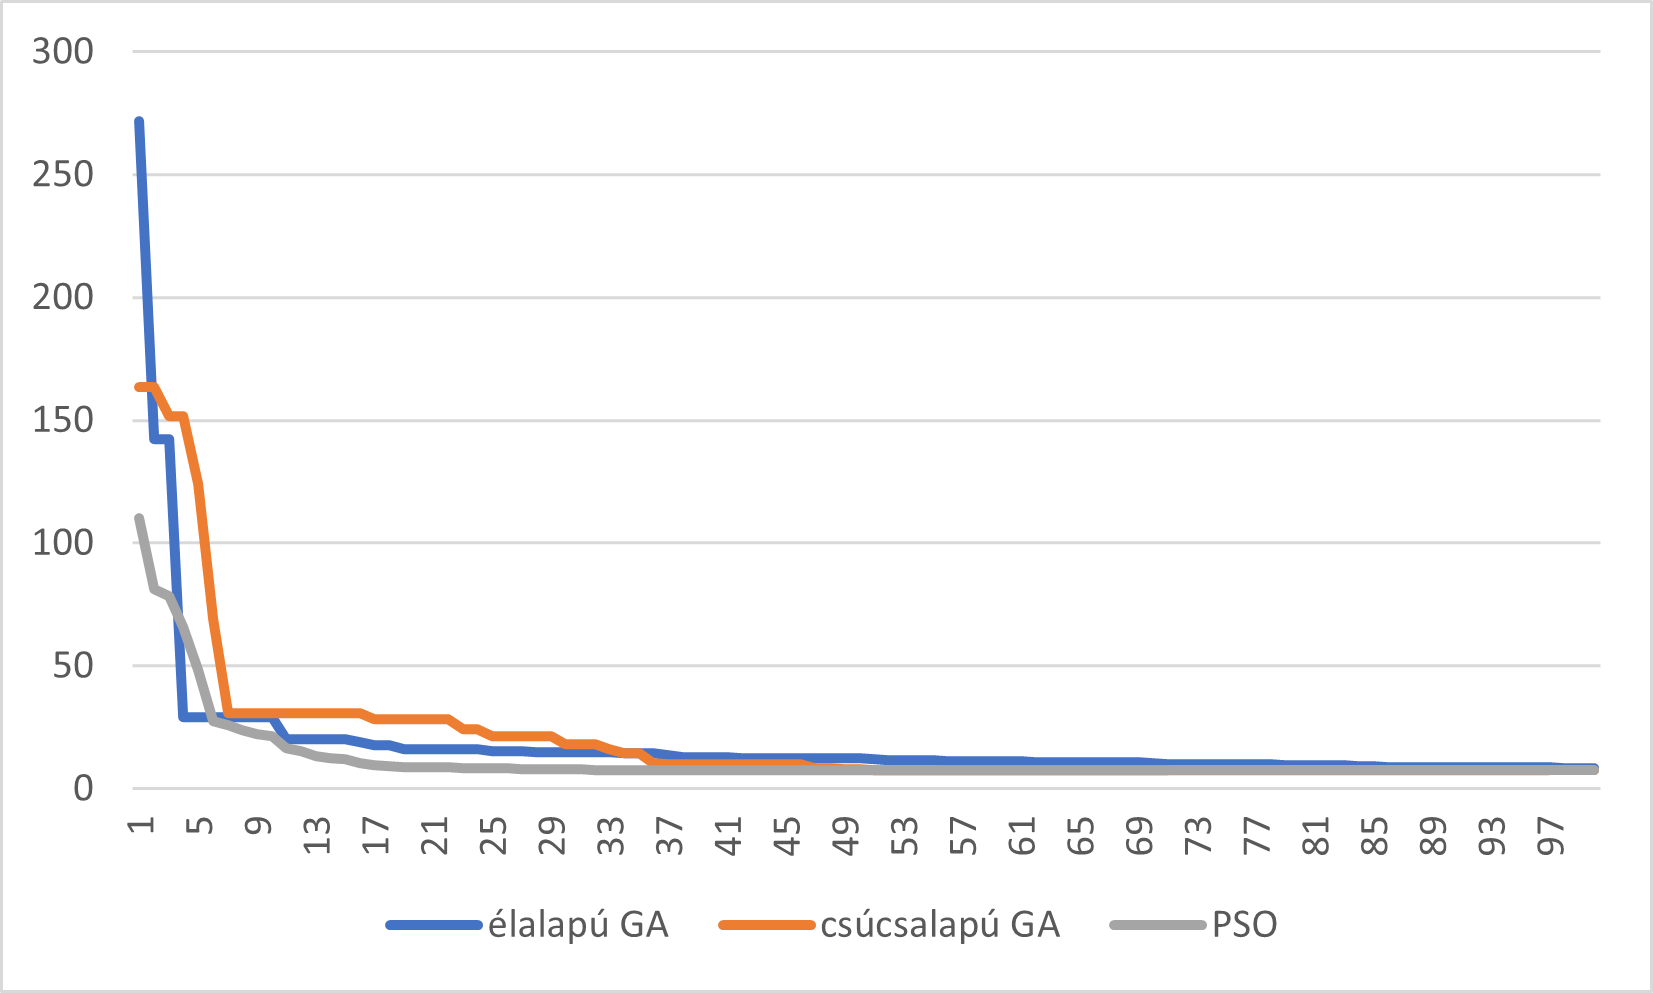
\includegraphics[width=0.30\linewidth]{25-8-20-cost}}
	\hspace{5pt}
	\subfigure[$H_{50,8,10}$]{
		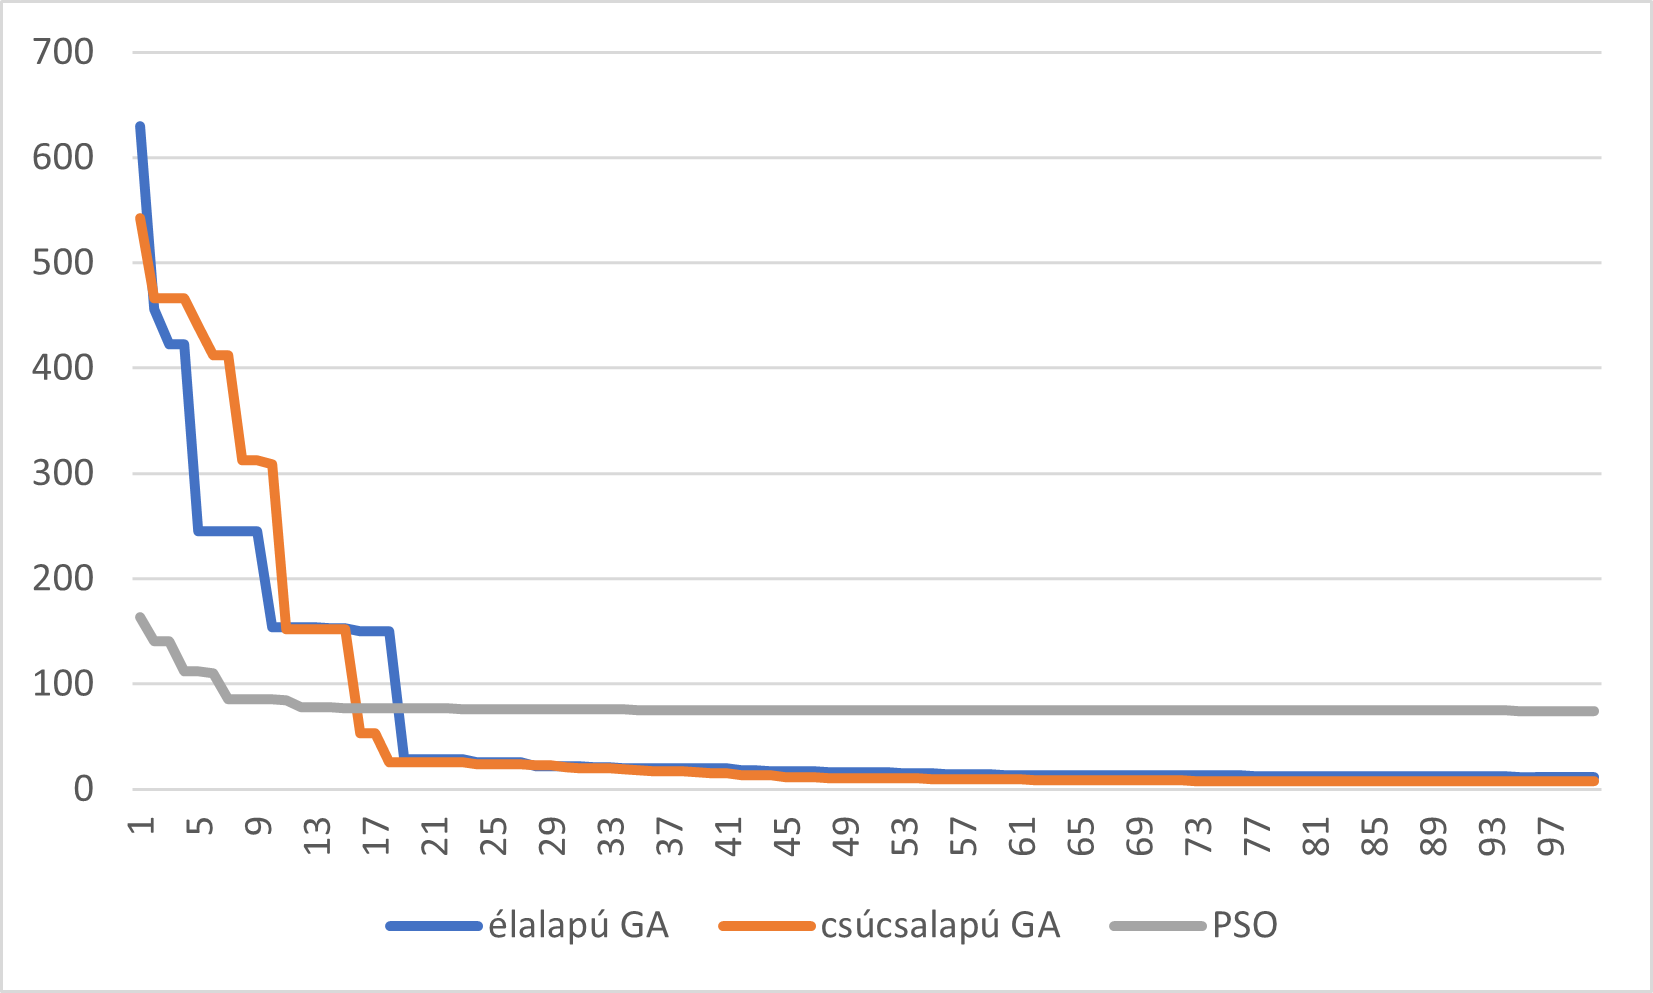
\includegraphics[width=0.30\linewidth]{50-8-10-cost}}
	\hspace{5pt}
	\subfigure[$H_{100,8,5}$]{
		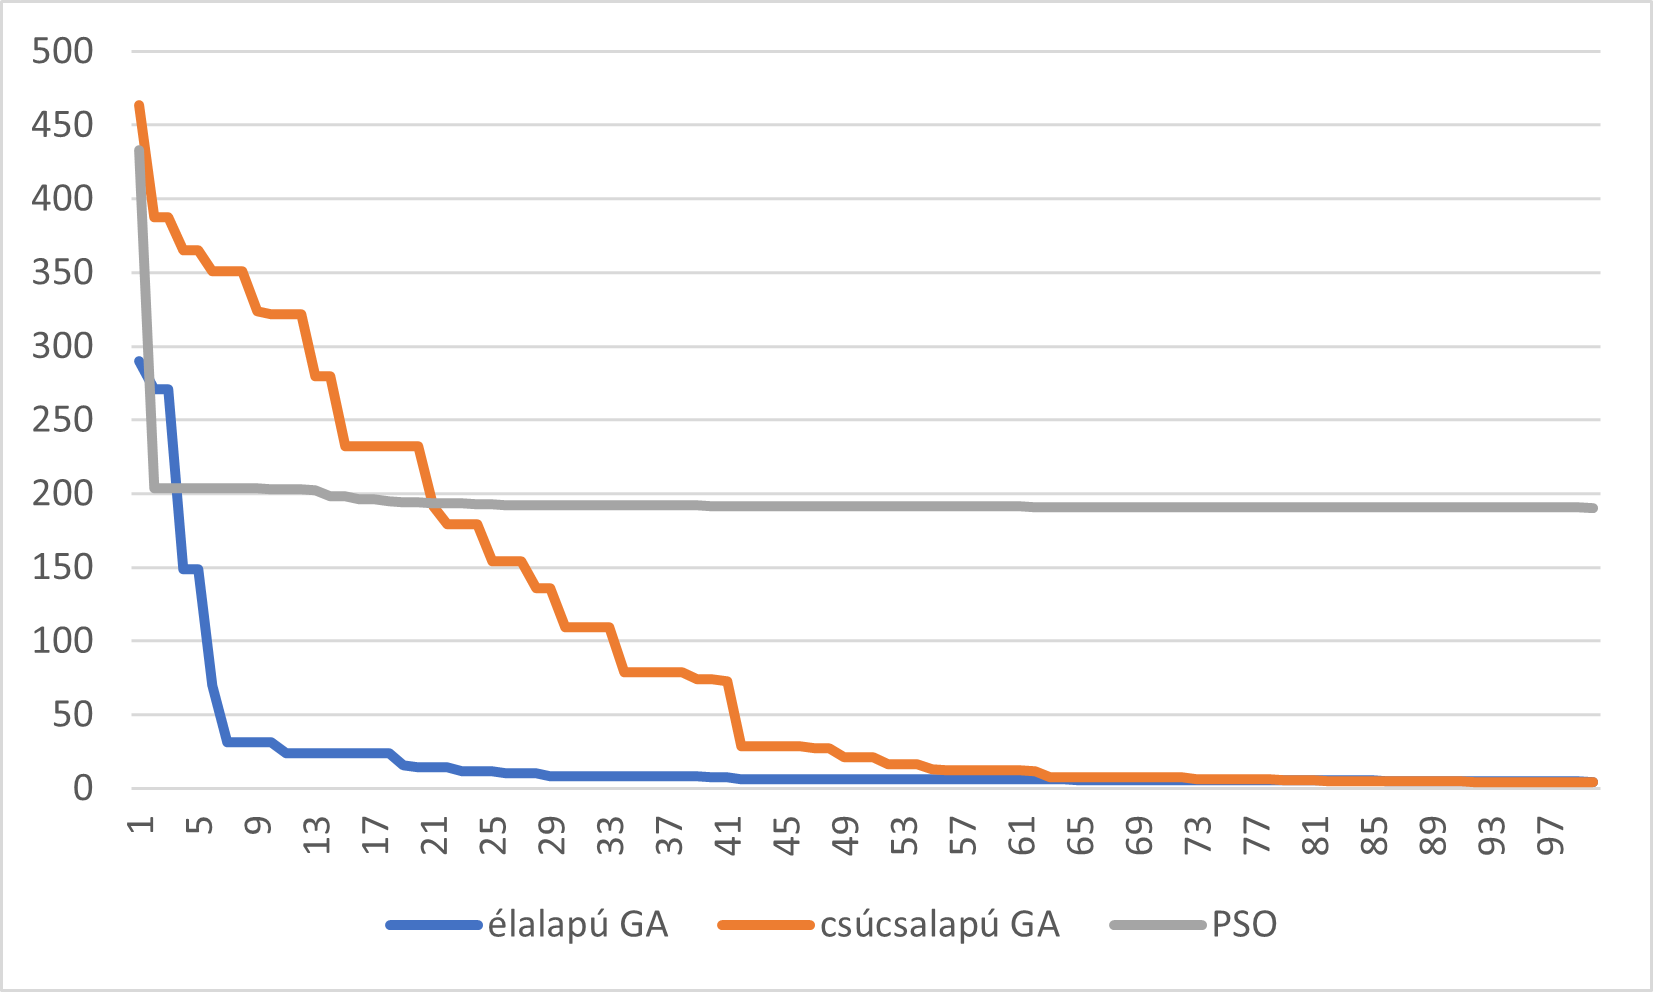
\includegraphics[width=0.30\linewidth]{100-8-5-cost}}
	\caption{Csúcsszám hatása a költségfüggvényre}
	\label{fig:node_size_cost}
\end{figure}

Úgy tűnik, hogy a a probléma ezen paraméterének megváltoztatása nagyban eltérően hat az egyes algoritmusokra. Míg az élalapú GA invariánsnak tűnik a csúcsszámra, addig a csúcsalapú GA esetében lassabb konvergenciához vezet, de végül mindketten hasonló minőségű ábrákat generálnak. Ezzel szemben a PSO teljesítményét abszolút negatívan befolyásolja, ha további csúcsokat adunk a problémához.

\begin{figure}[H]
	\centering
	\subfigure[$H_{25,8,20}$]{
		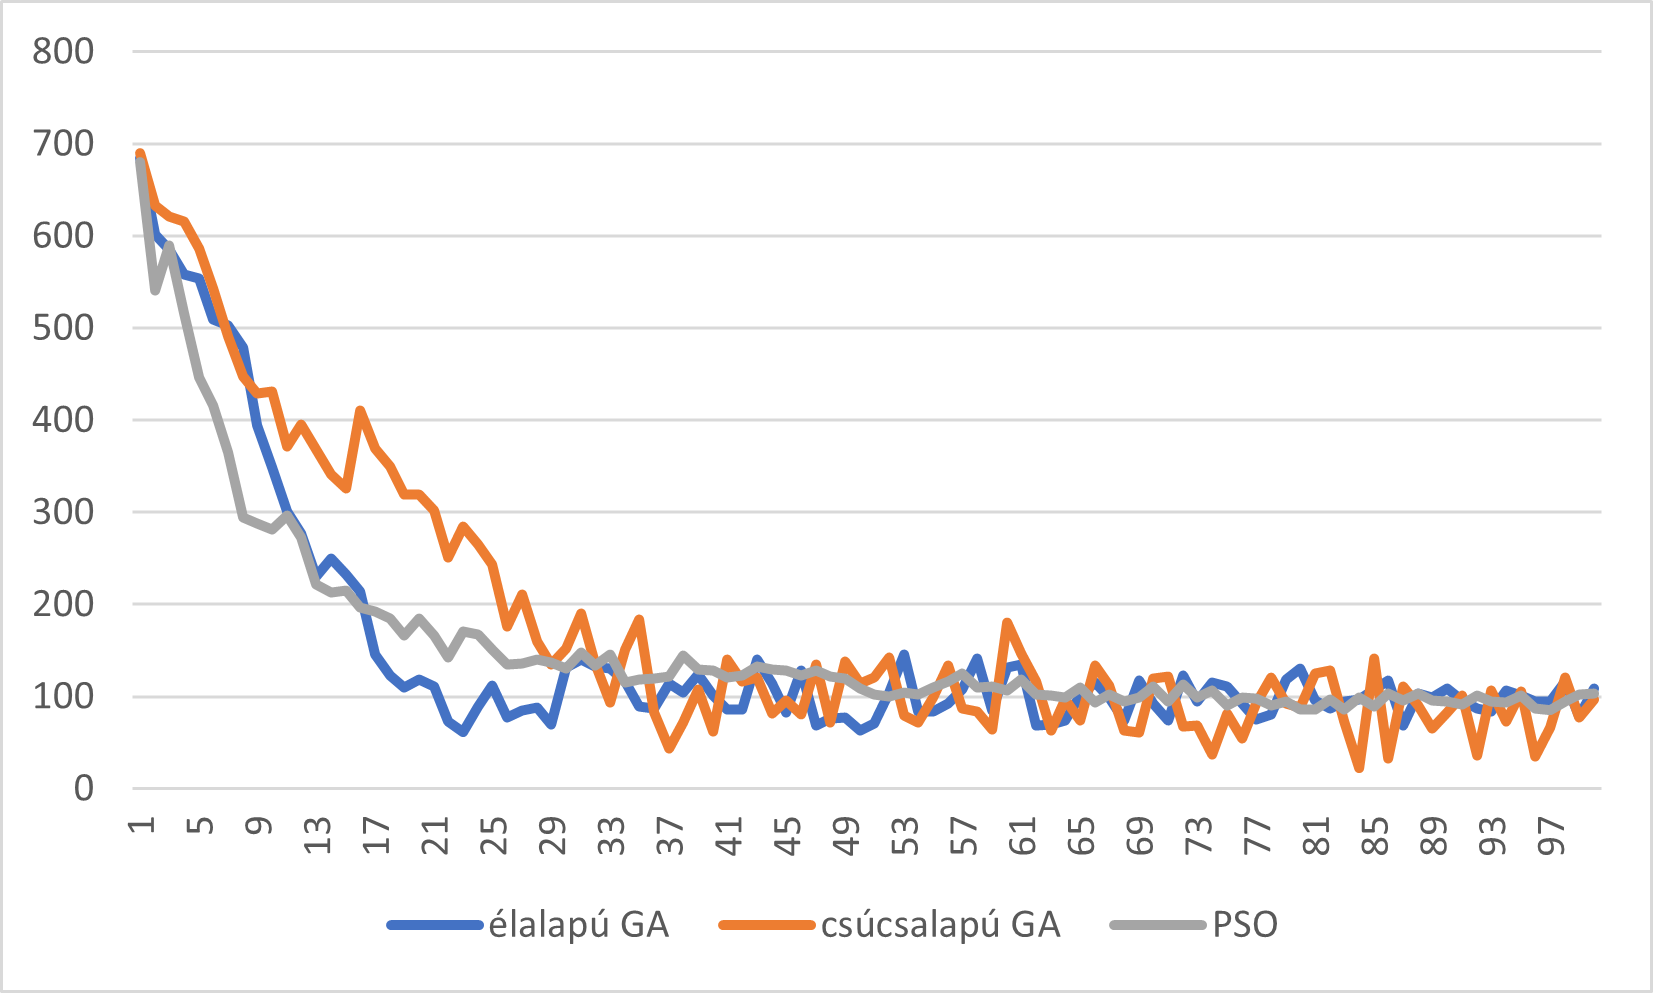
\includegraphics[width=0.30\linewidth]{25-8-20-cost-mean}}
	\hspace{5pt}
	\subfigure[$H_{50,8,10}$]{
		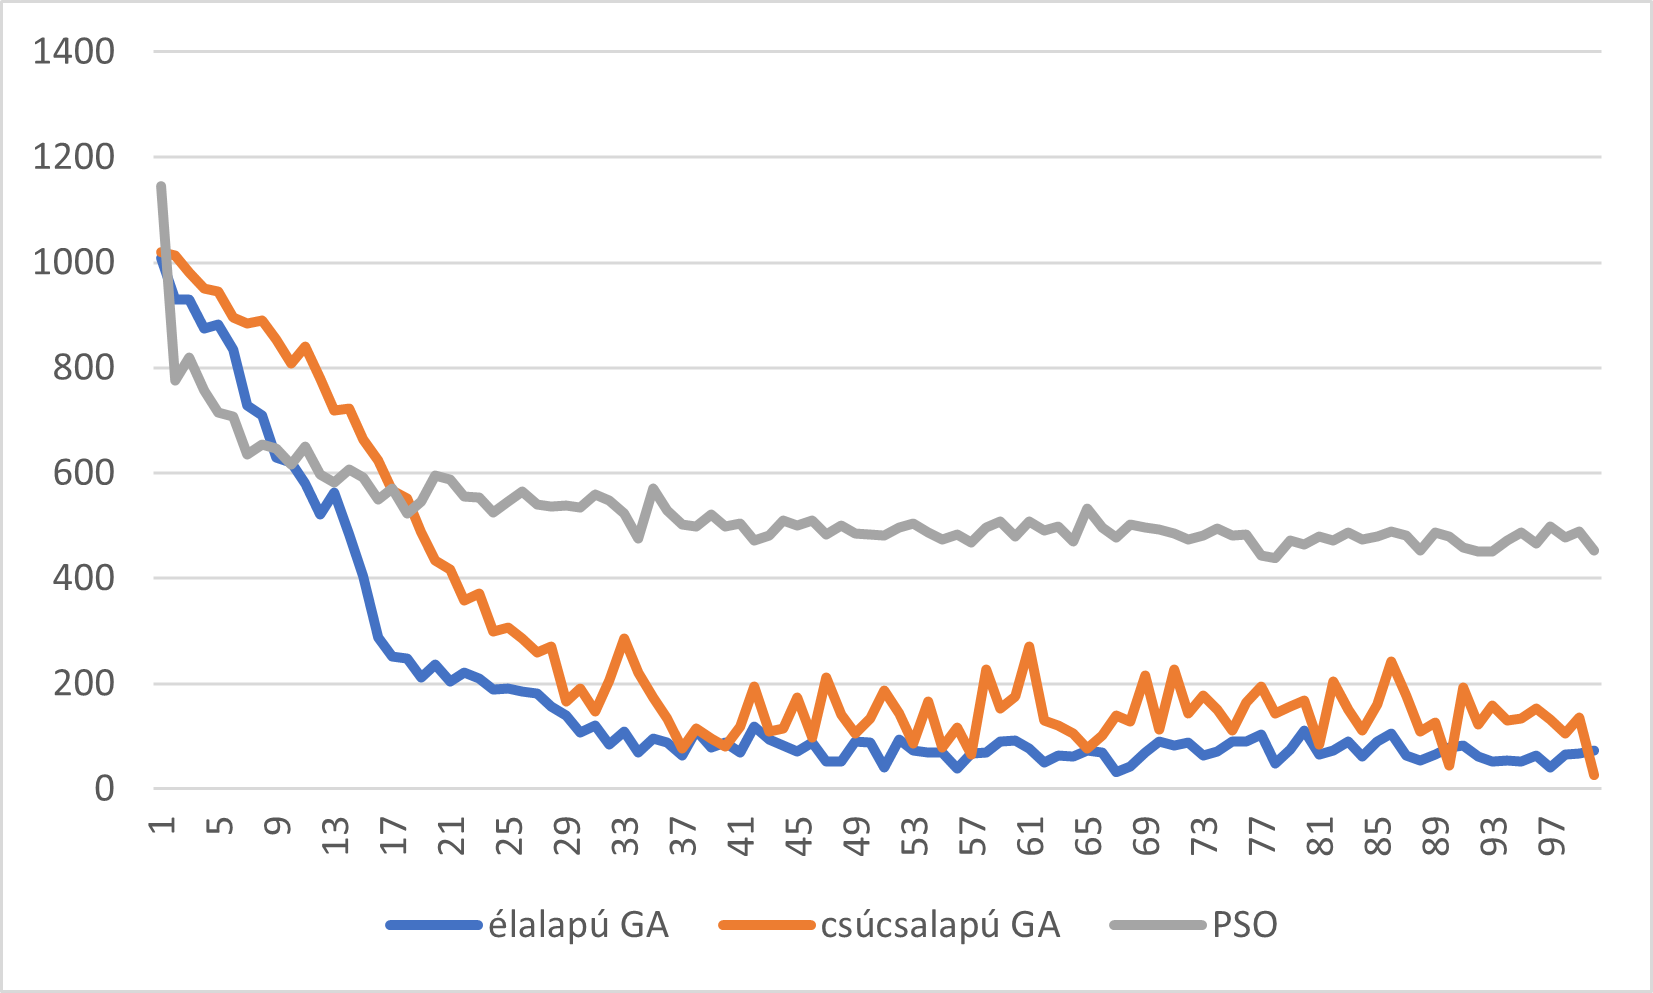
\includegraphics[width=0.30\linewidth]{50-8-10-cost-mean}}
	\hspace{5pt}
	\subfigure[$H_{100,8,5}$]{
		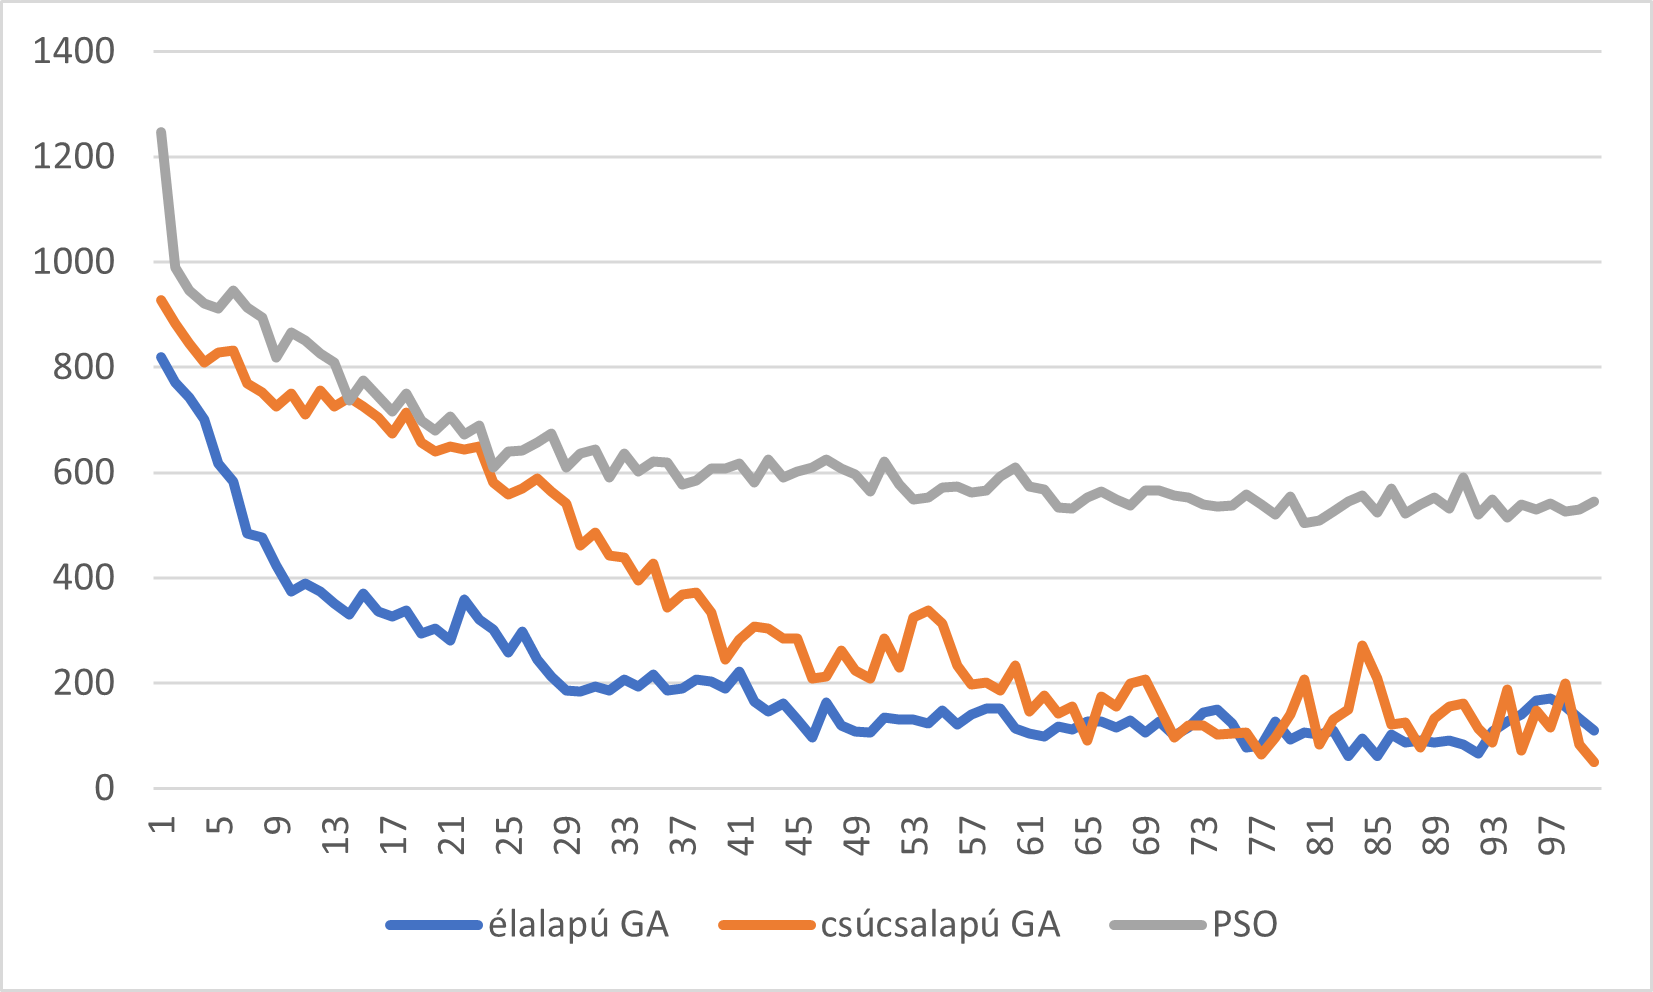
\includegraphics[width=0.30\linewidth]{100-8-5-cost-mean}}
	\caption{Csúcsszám hatása a megoldáspopuláció költségfüggvényének átlagára}
	\label{fig:node_size_cost_mean}
\end{figure}

\begin{figure}[H]
	\centering
	\subfigure[$H_{25,8,20}$]{
		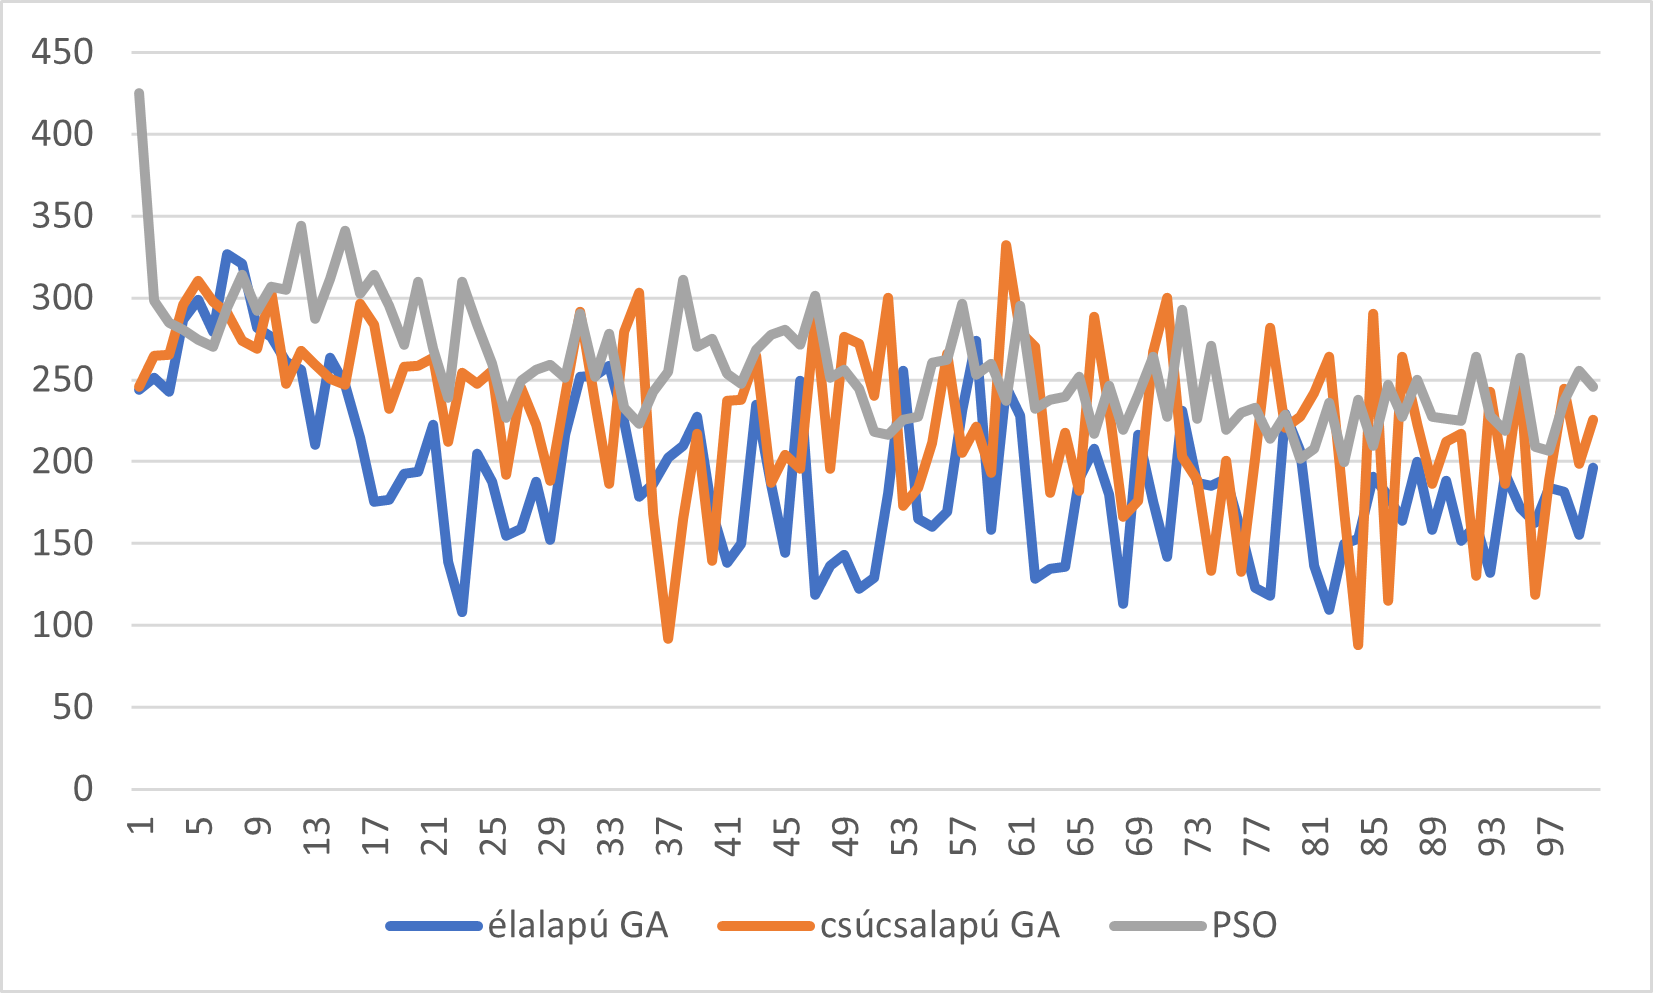
\includegraphics[width=0.30\linewidth]{25-8-20-cost-std}}
	\hspace{5pt}
	\subfigure[$H_{50,8,10}$]{
		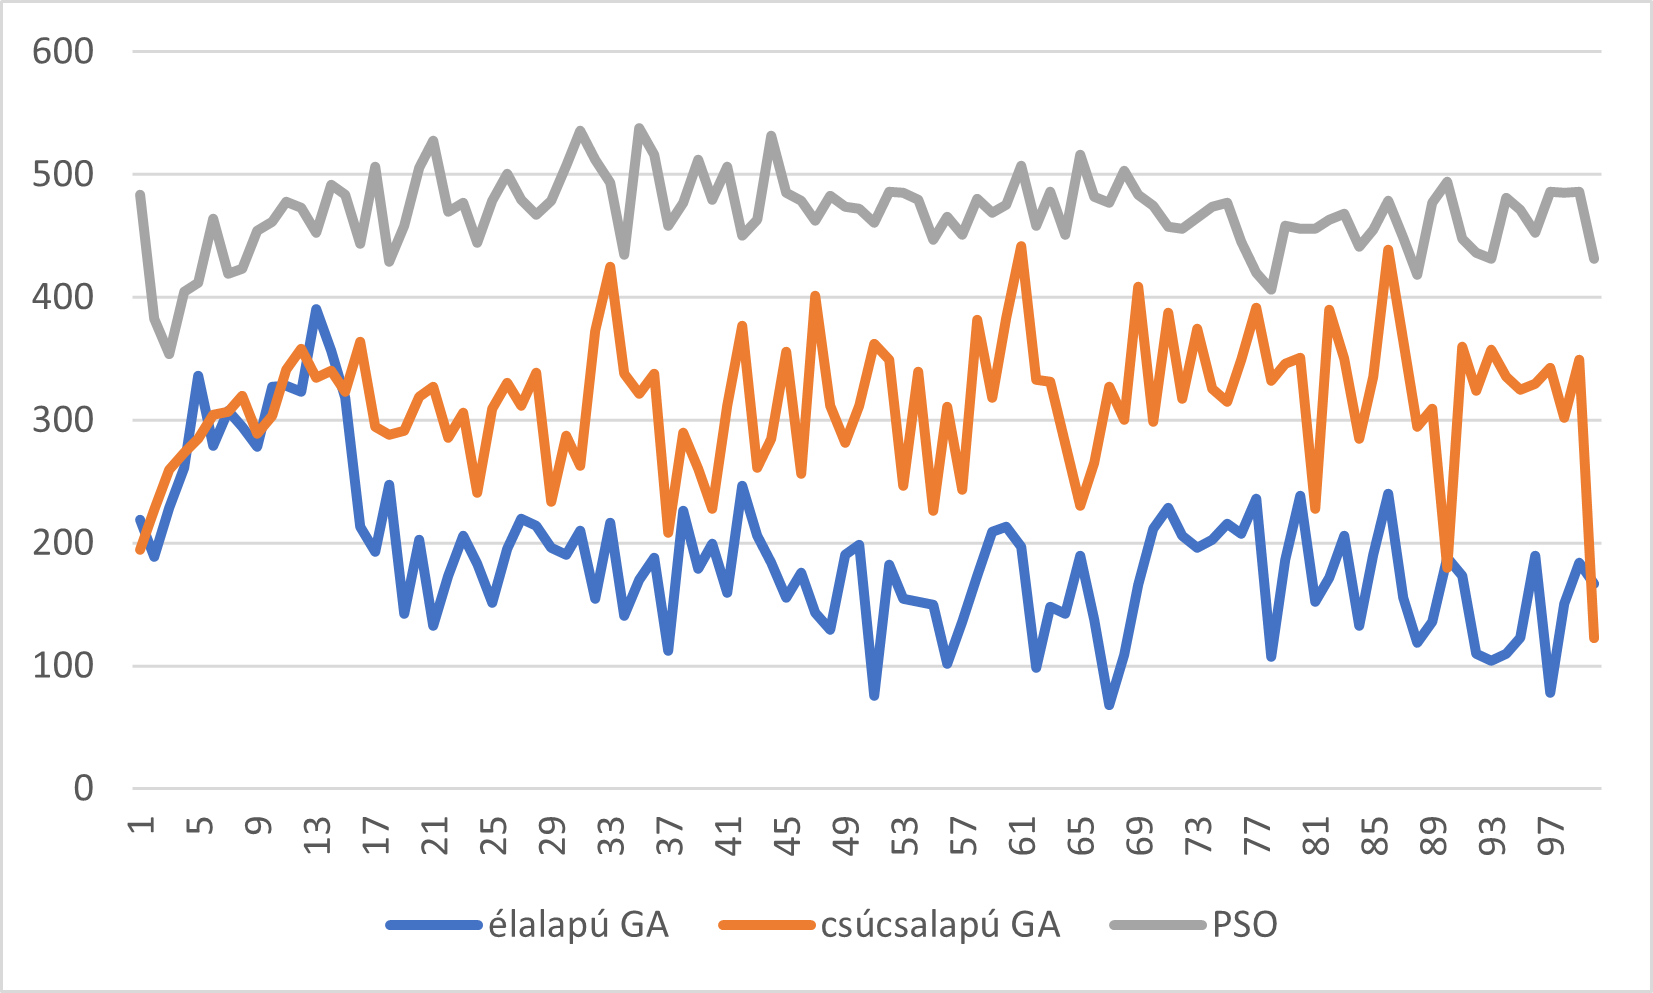
\includegraphics[width=0.30\linewidth]{50-8-10-cost-std}}
	\hspace{5pt}
	\subfigure[$H_{100,8,5}$]{
		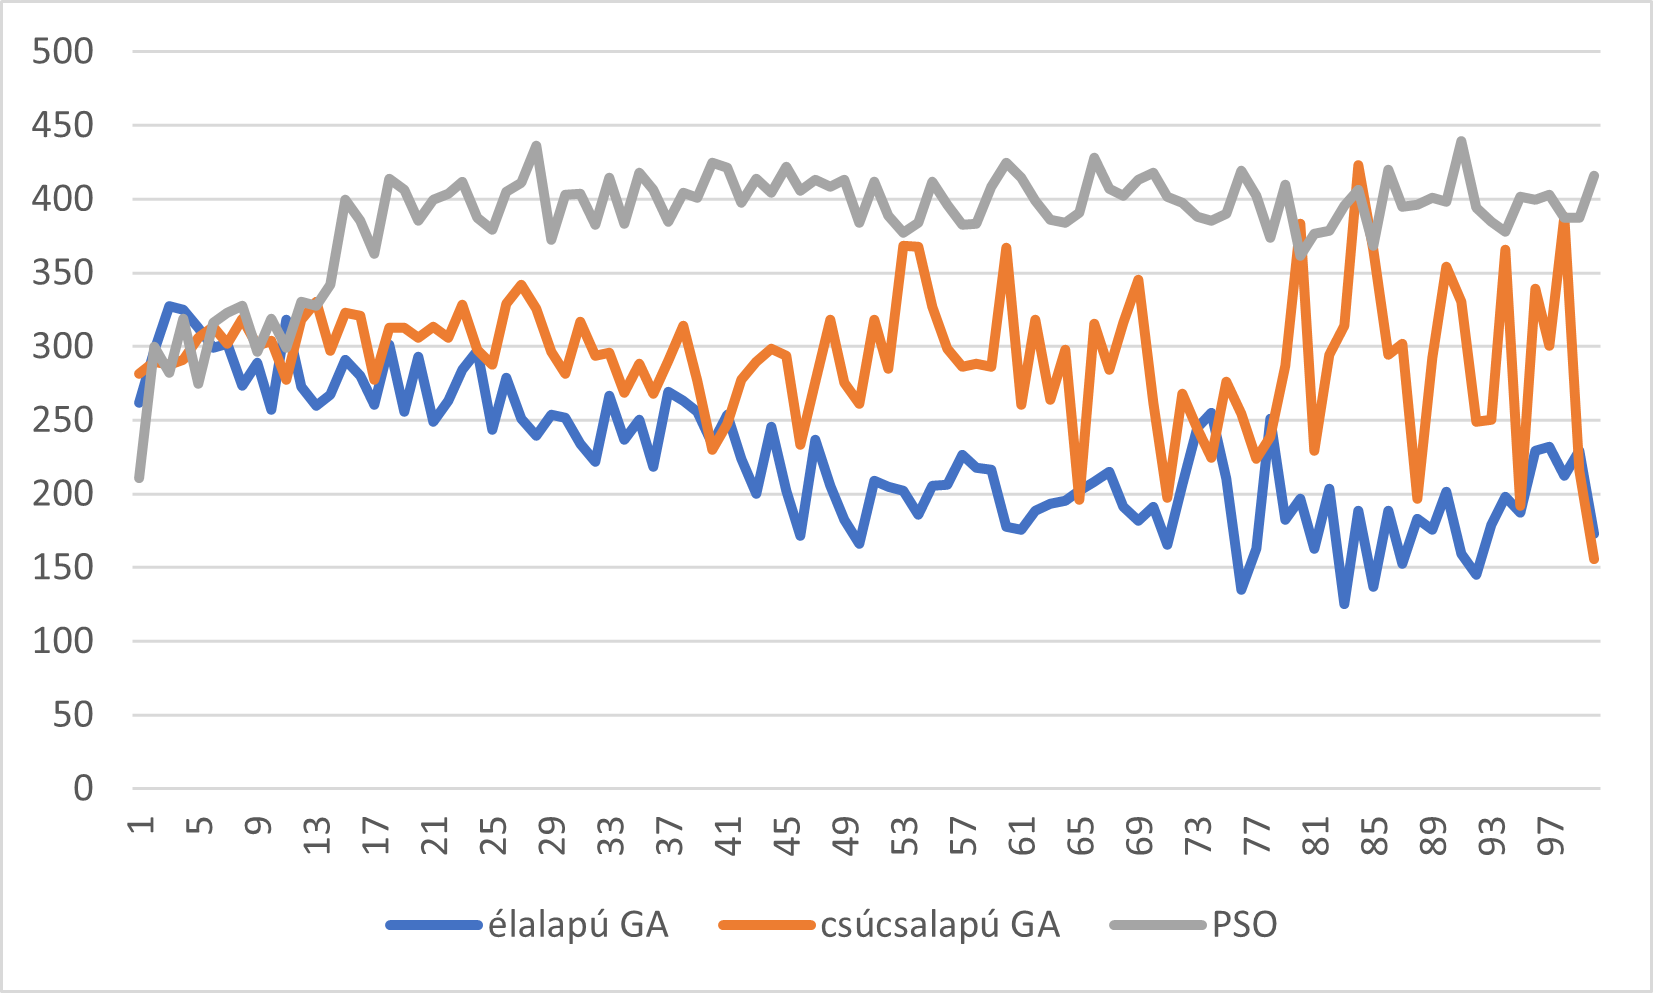
\includegraphics[width=0.30\linewidth]{100-8-5-cost-std}}
	\caption{Csúcsszám hatása a megoldáspopuláció költségfüggvényének szórására}
	\label{fig:node_size_cost_std}
\end{figure}

Nem meglepő a korábbiak alapján, hogy az optimalizáció során átlagosan a kettő GA algoritmus megoldáspopulációja hasonlóan jó eredményt ér el, míg a PSO-ról ez már nem mondható el. A szórást vizsgálva azt mondhatjuk el, hogy a PSO során kapott költségfüggvények jóval nagyobb kilengéseket mutatnak, de a csúcsalapú GA is kevésbé stabil, mint az élalapú.

\subsubsection{Élszám növelése}

Élszámok esetén $H_{25,8,20}$-at, $H_{25,16,20}$-at és $H_{25,32,20}$-at vettem górcső alá.

\begin{figure}[H]
	\centering
	\subfigure[$H_{25,8,20}$]{
		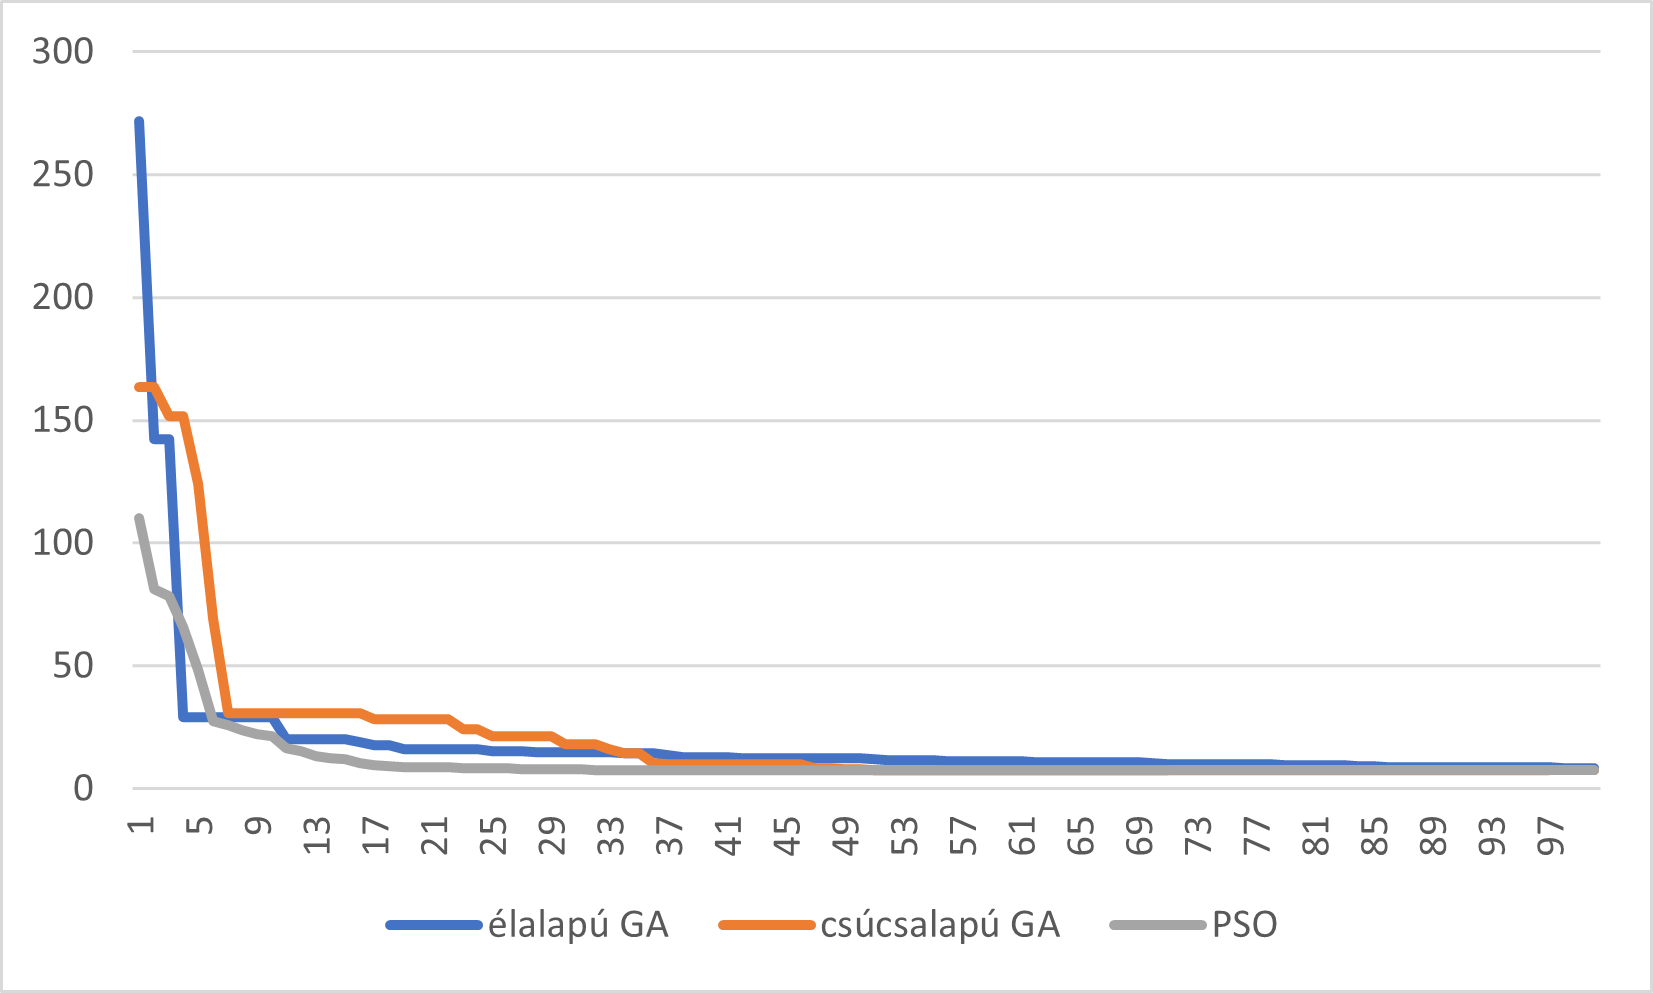
\includegraphics[width=0.30\linewidth]{25-8-20-cost}}
	\hspace{5pt}
	\subfigure[$H_{25,16,20}$]{
		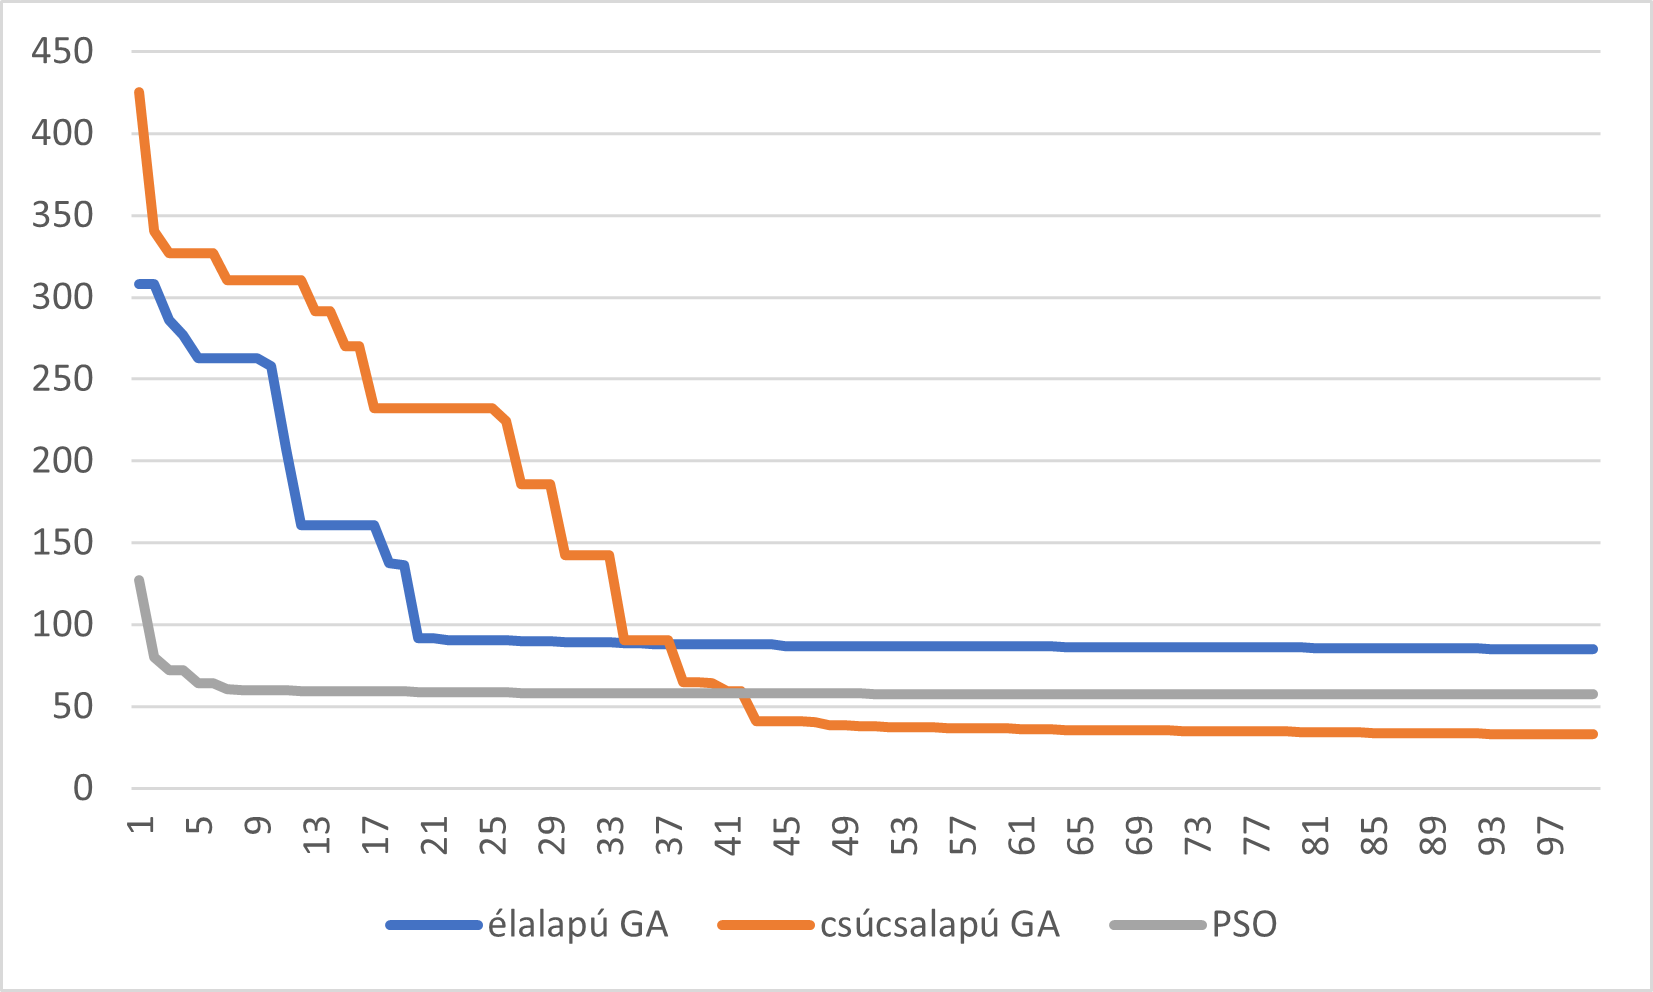
\includegraphics[width=0.30\linewidth]{25-16-20-cost}}
	\hspace{5pt}
	\subfigure[$H_{25,32,20}$]{
		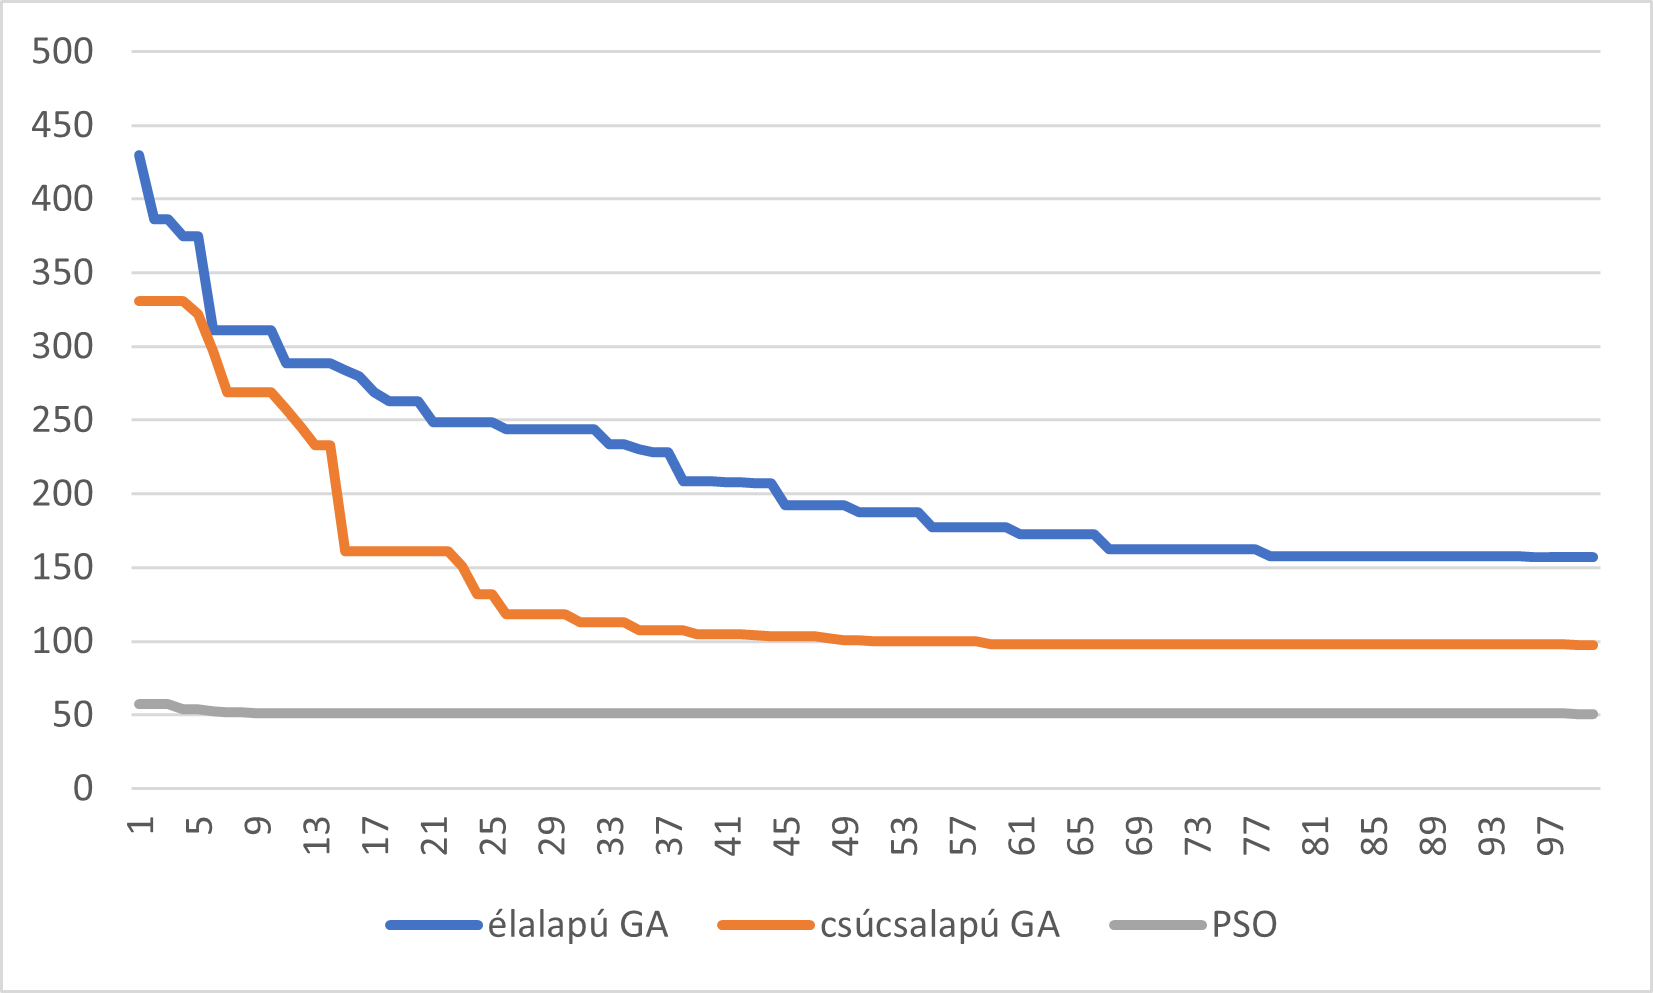
\includegraphics[width=0.30\linewidth]{25-32-20-cost}}
	\caption{Élszám hatása a költségfüggvényre}
\end{figure}

Ebben az esetben a csúcsszámokkal pont ellentétes konklúzióra juthatunk, a PSO-t érinti legkevésbé az élszám növelése, az élalapú GA-t pedig a legnagyobb mértékben. Érdemes megemlíteni, hogy míg a csúcsszám változtatásával az elérhető költségfüggvény nagyságrendje nem változott, ez már nem áll meg az élszám esetén, ahol még a a legjobban eredményt adó módszer teljesítménye is észrevehetően romlik. Meglepő módon átlagosan nem a PSO operál a minimális költségfüggvényű (és szórású) populációval, hanem a csúcsalapú GA.

\begin{figure}[H]
	\centering
	\subfigure[$H_{25,8,20}$]{
		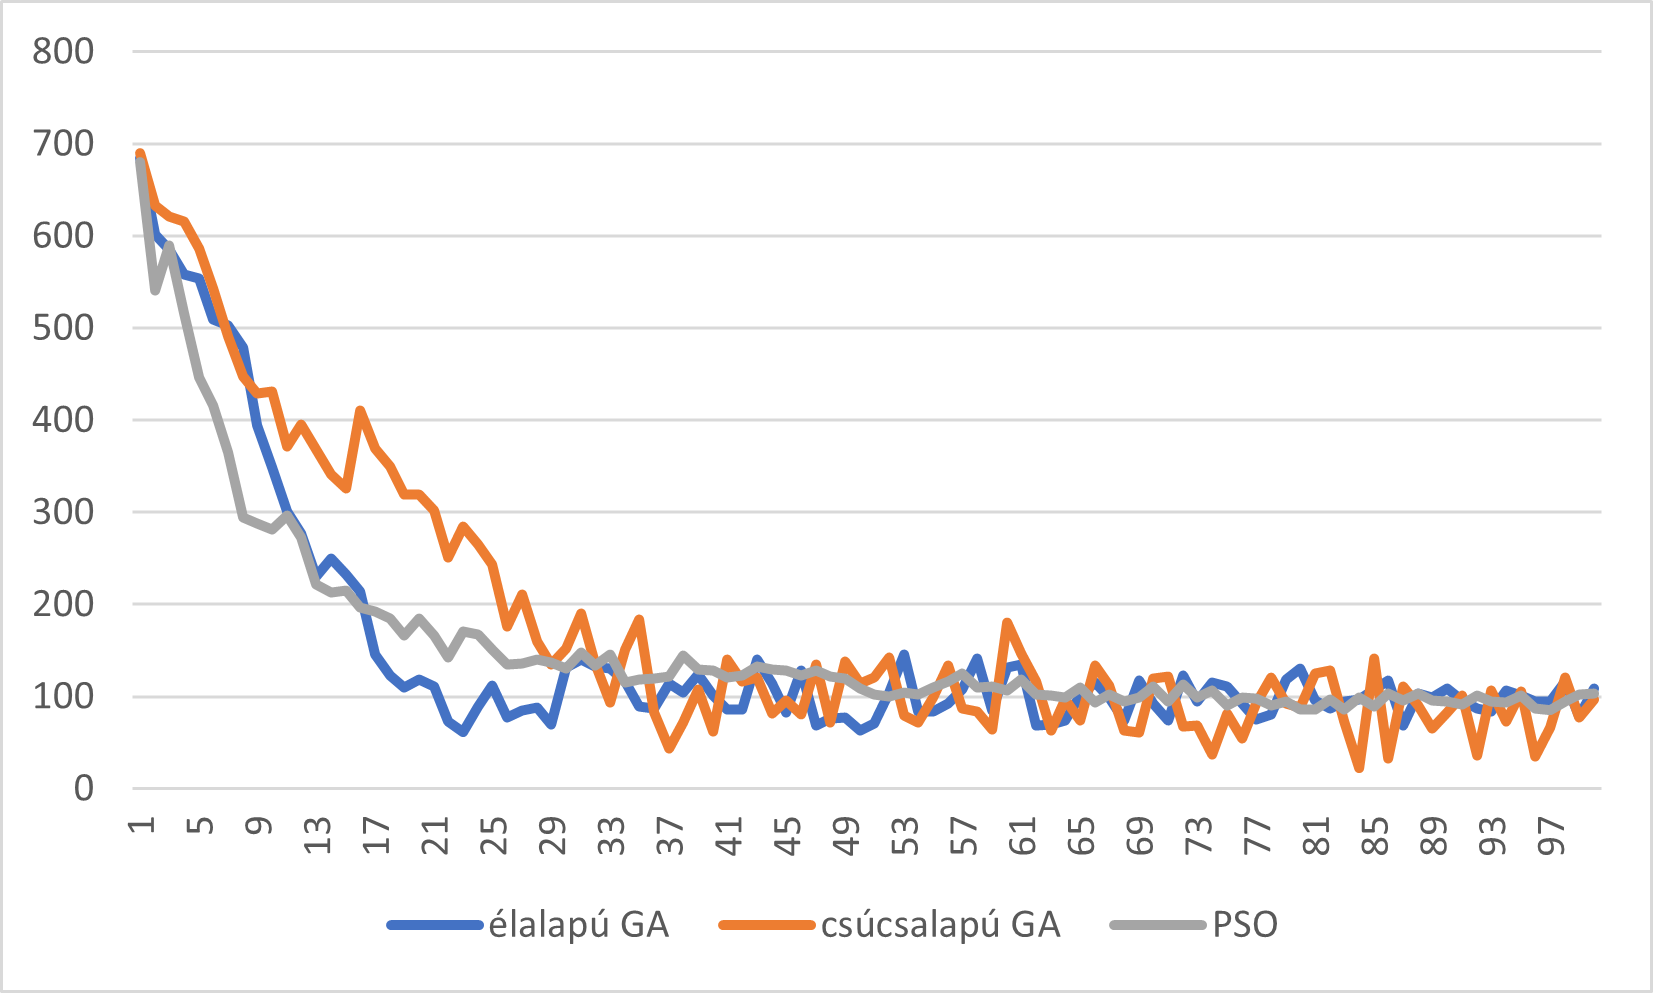
\includegraphics[width=0.30\linewidth]{25-8-20-cost-mean}}
	\hspace{5pt}
	\subfigure[$H_{25,16,20}$]{
		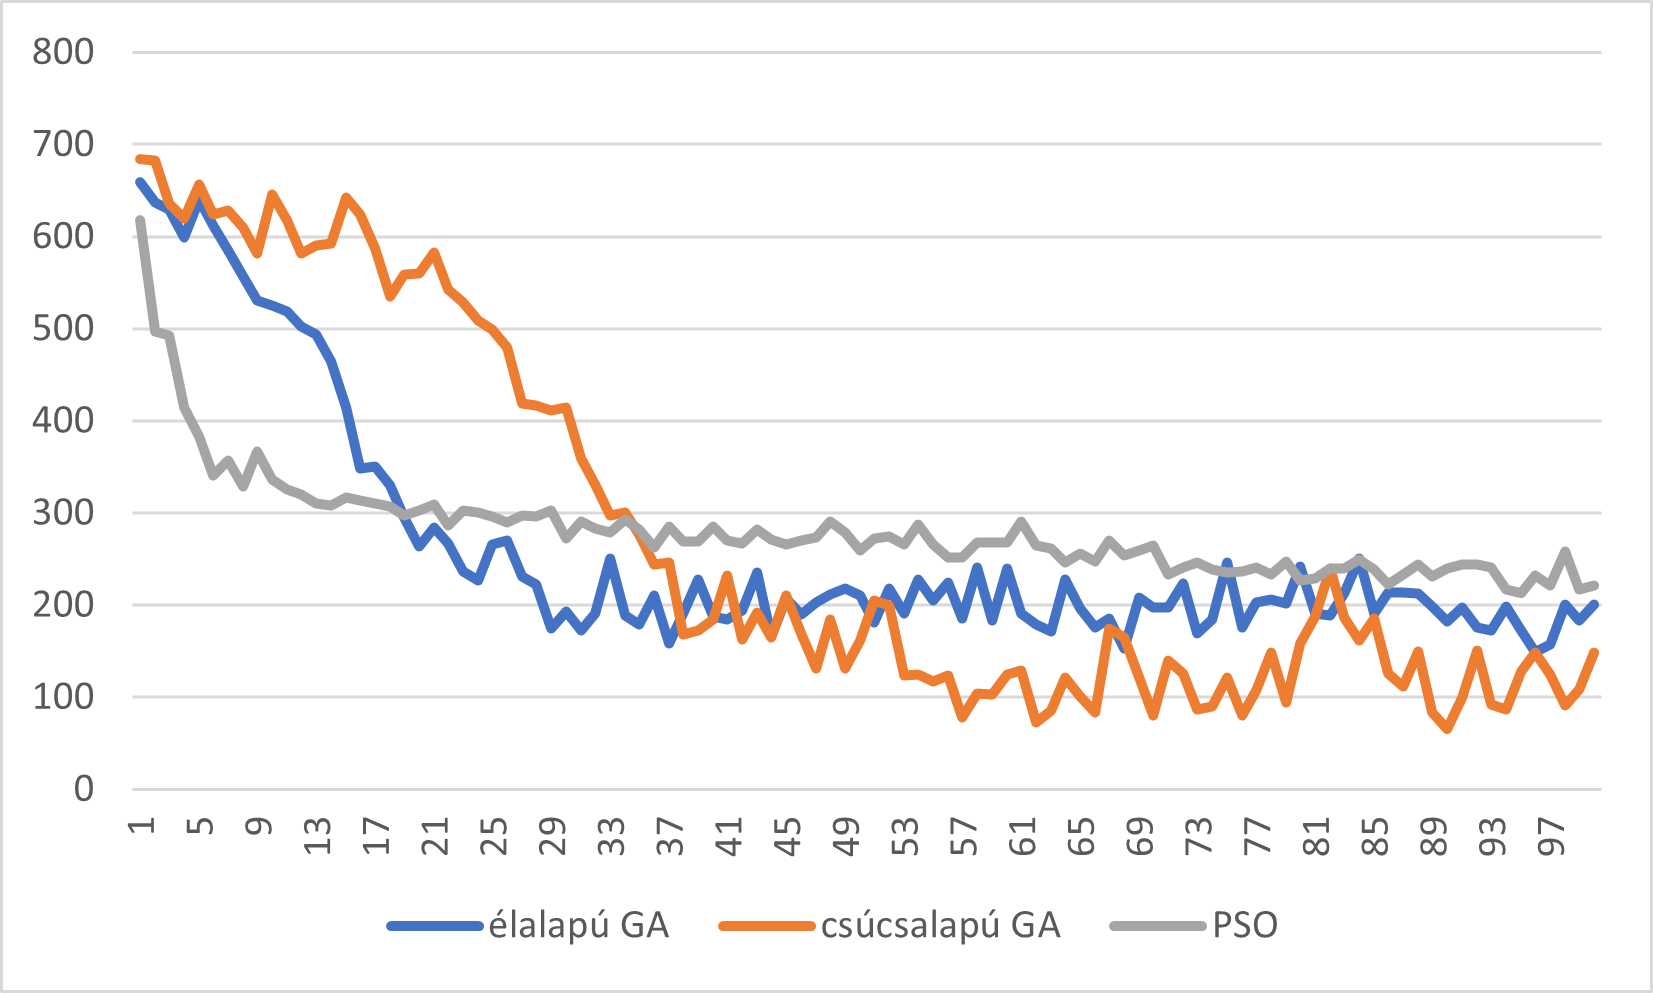
\includegraphics[width=0.30\linewidth]{25-16-20-cost-mean}}
	\hspace{5pt}
	\subfigure[$H_{25,32,20}$]{
		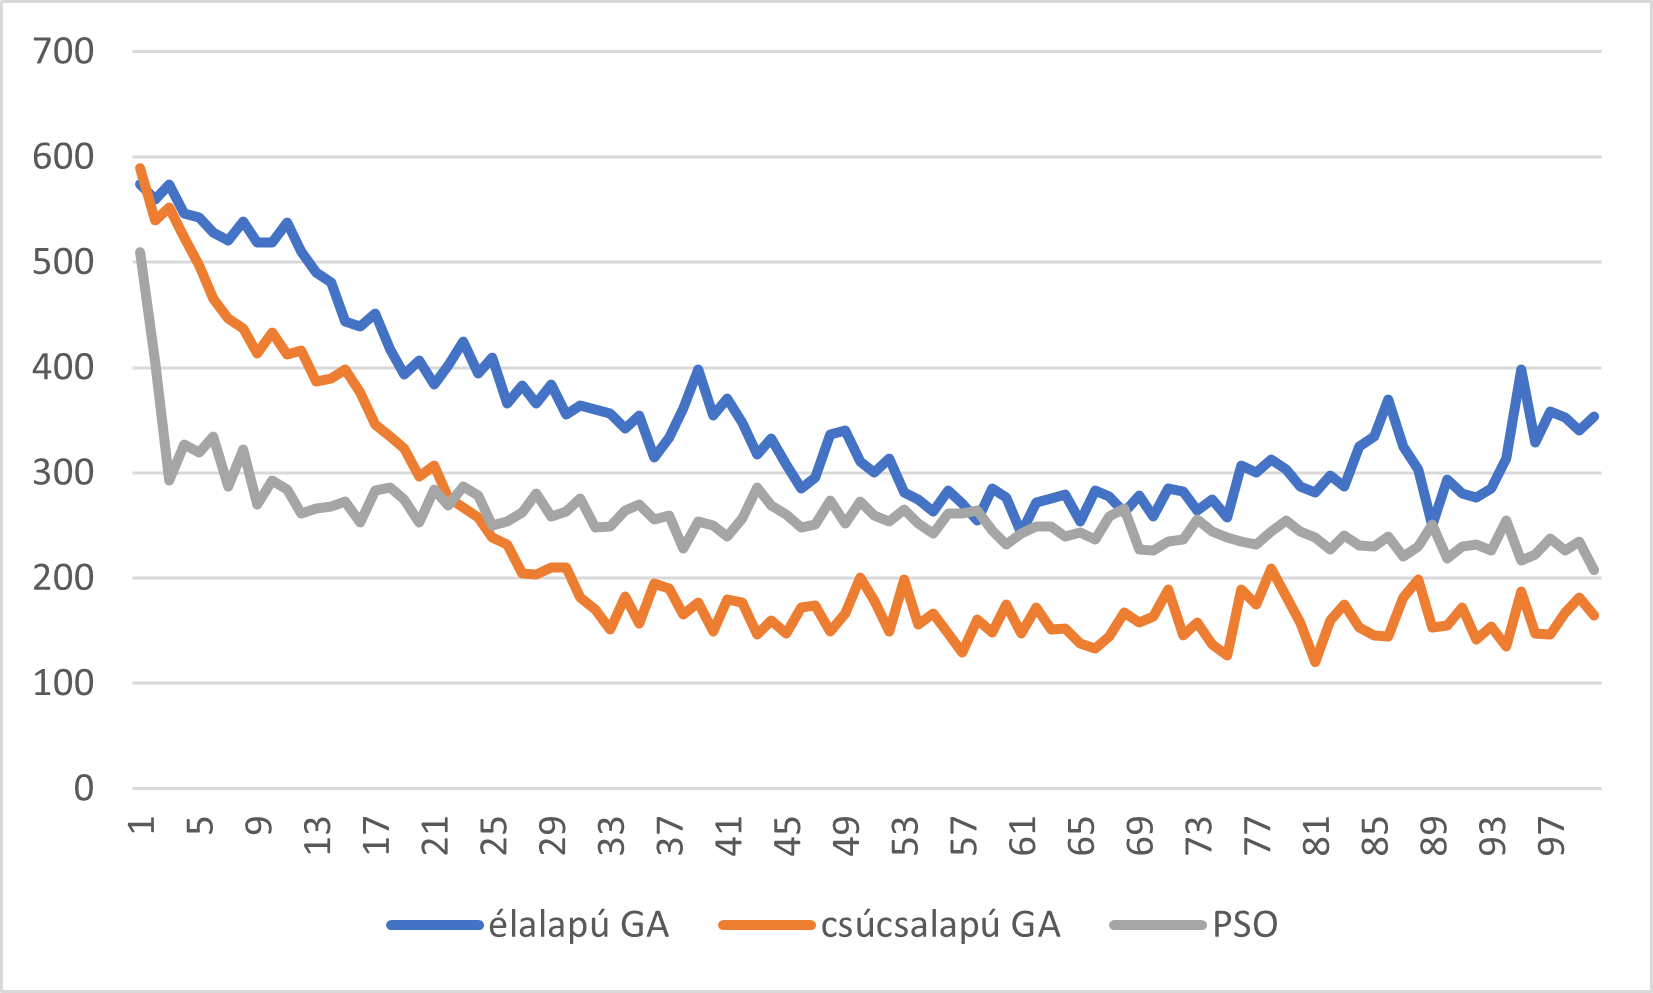
\includegraphics[width=0.30\linewidth]{25-32-20-cost-mean}}
	\caption{Élszám hatása a megoldáspopuláció költségfüggvényének átlagára}
\end{figure}

\begin{figure}[H]
	\centering
	\subfigure[$H_{25,8,20}$]{
		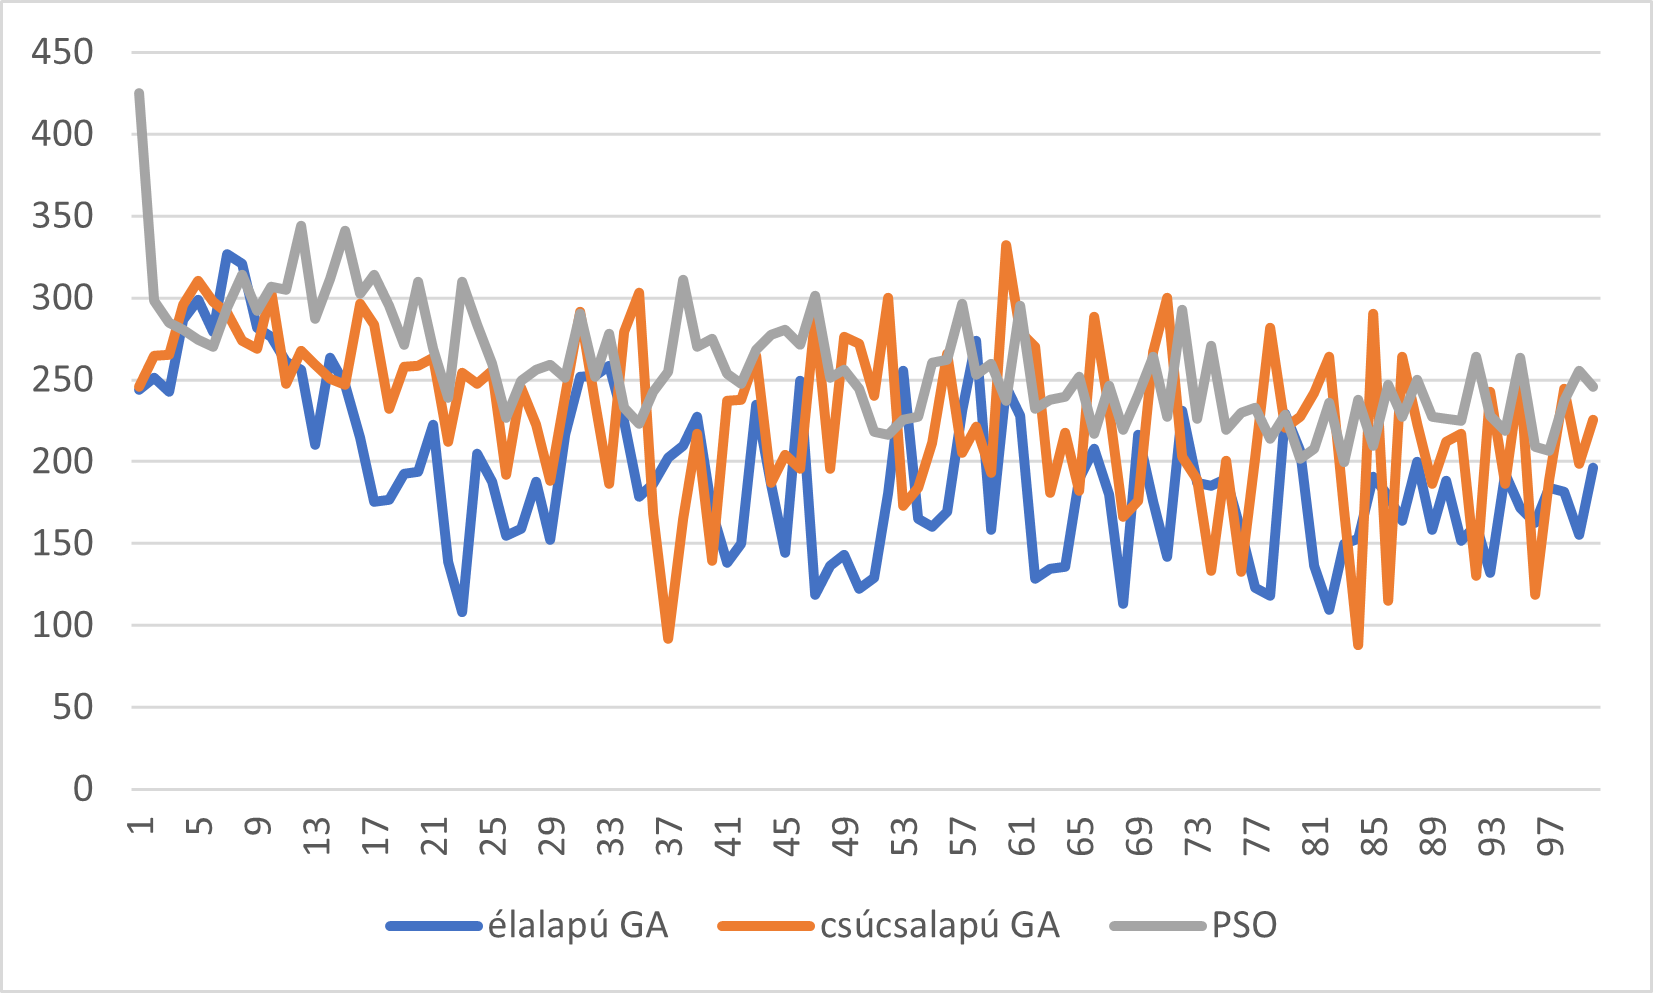
\includegraphics[width=0.30\linewidth]{25-8-20-cost-std}}
	\hspace{5pt}
	\subfigure[$H_{25,16,20}$]{
		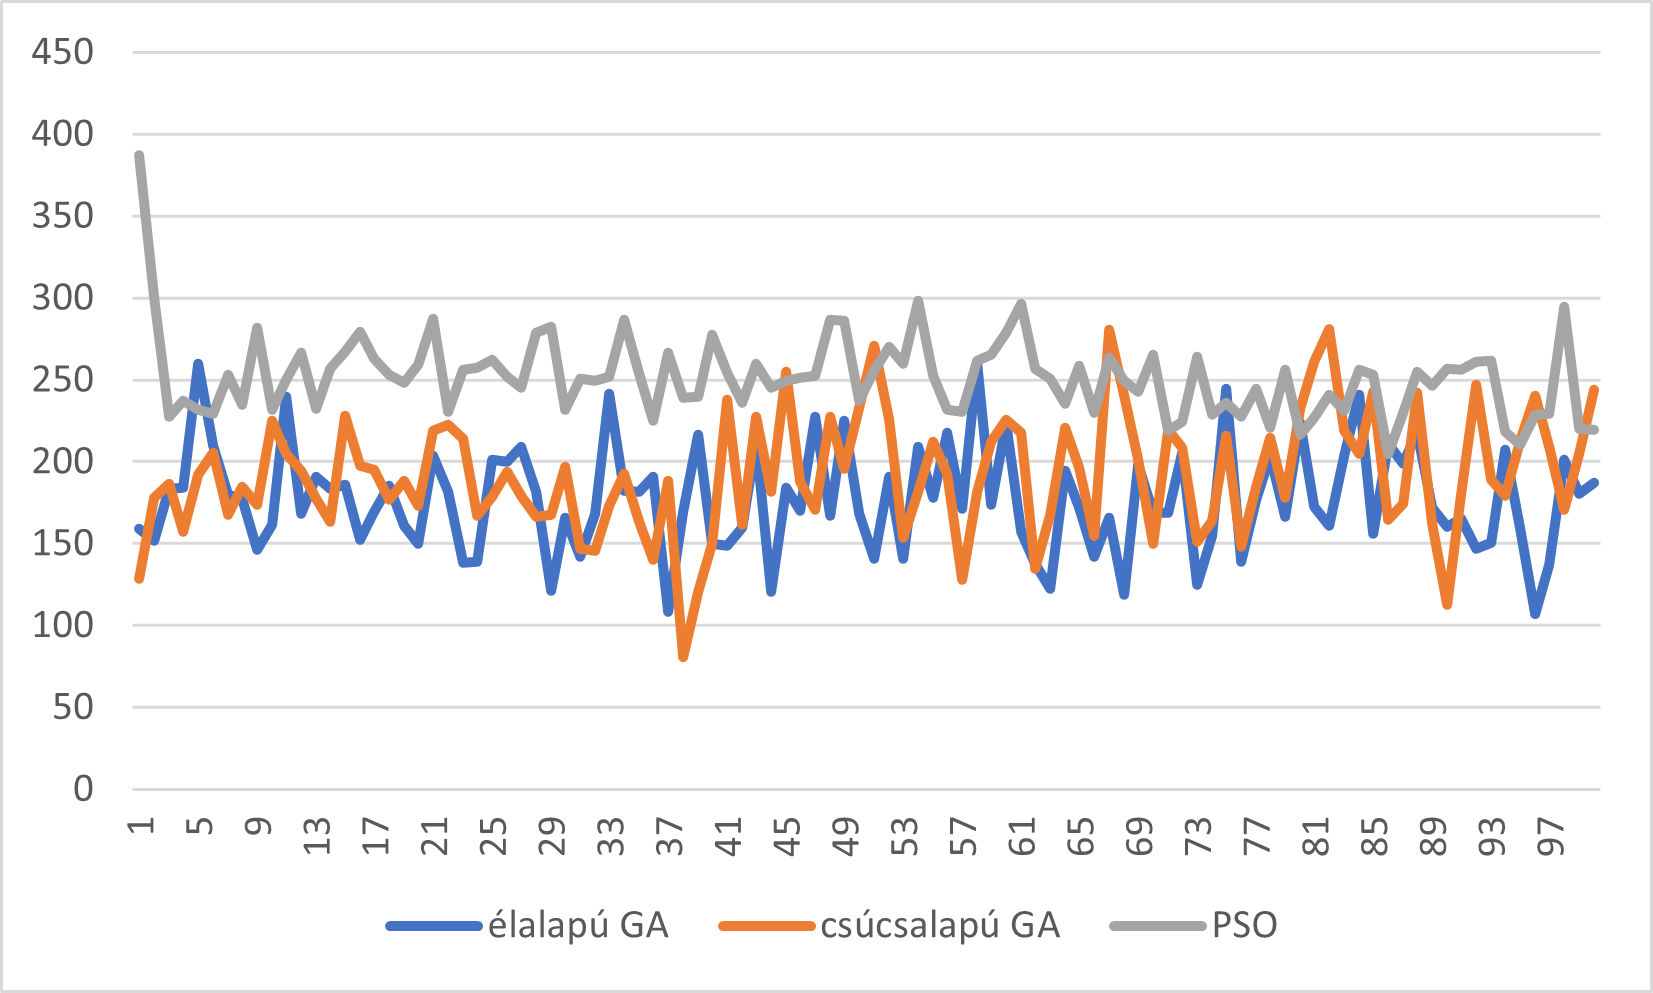
\includegraphics[width=0.30\linewidth]{25-16-20-cost-std}}
	\hspace{5pt}
	\subfigure[$H_{25,32,20}$]{
		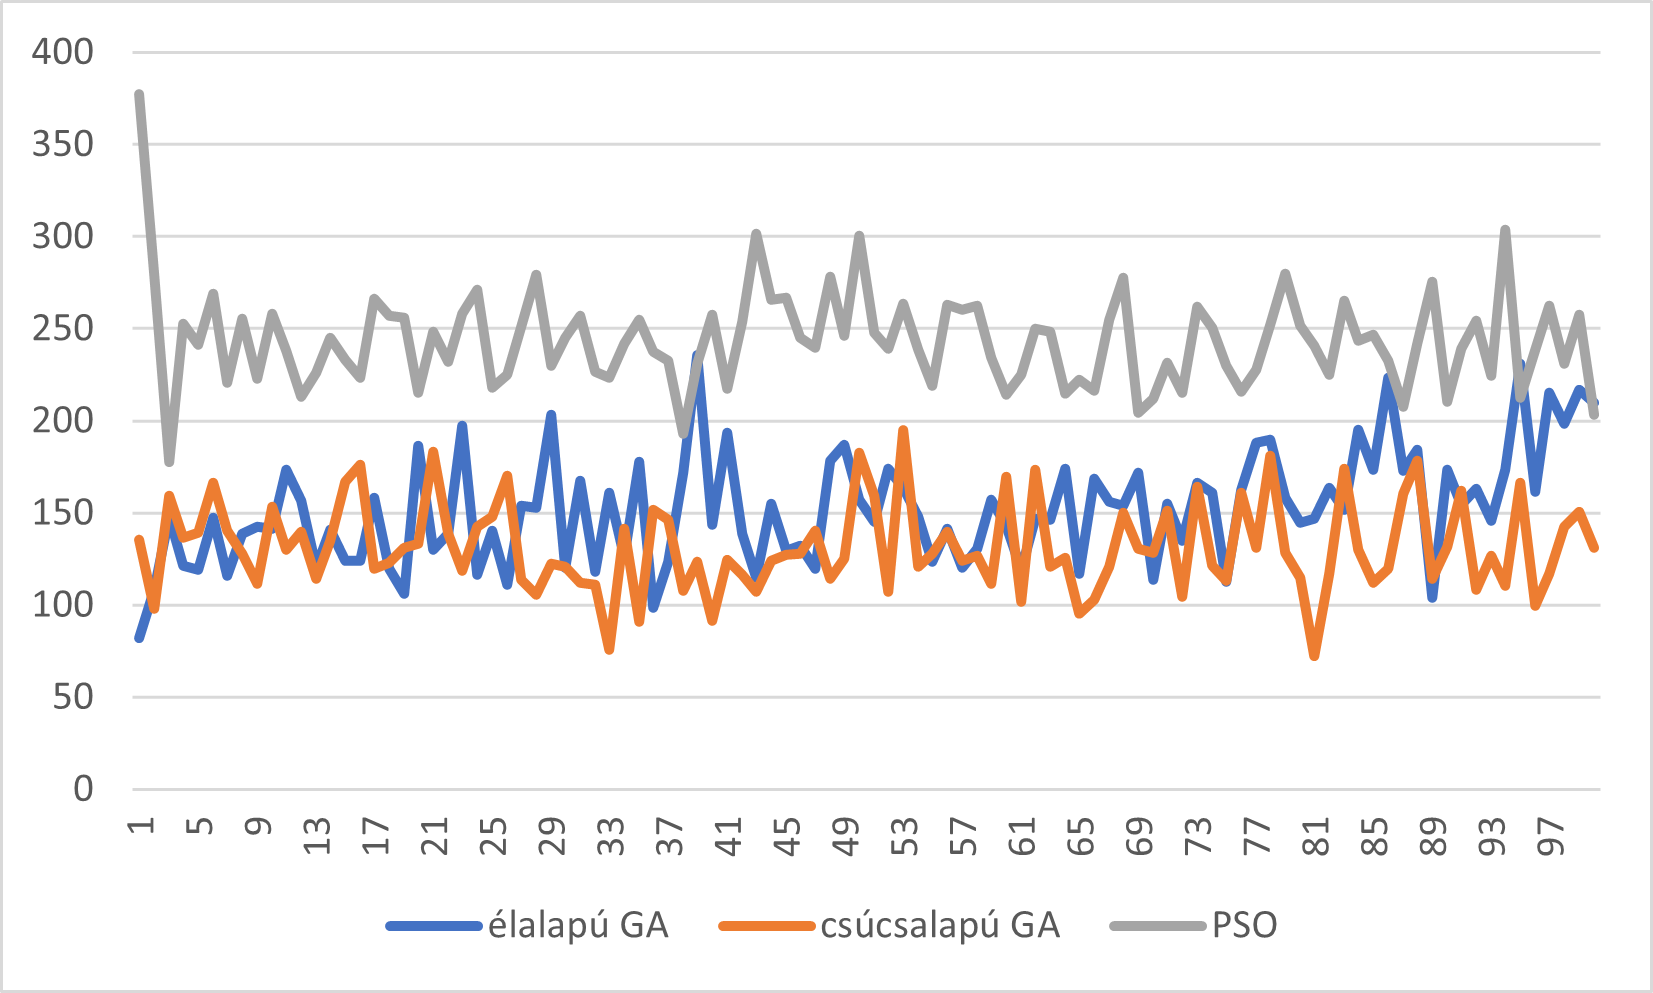
\includegraphics[width=0.30\linewidth]{25-32-20-cost-std}}
	\caption{Élszám hatása a megoldáspopuláció költségfüggvényének szórására}
\end{figure}

\subsubsection{Csúcs- és élszám együttes növelése}

Mivel az előző két mérés során a csúcsszám és az élszám növelésével eltérő módszerek kerültek ki győztesként, ezért felmerül a kérdés, hogy mi történik, mikor mindkettőt egyszerre növeljük. Ehhez a korábbi mérések kombinációjával előálló $H_{25,8,20}$, $H_{50,16,10}$ és $H_{100,32,5}$ hipergráfokat használom fel.

\begin{figure}[H]
	\centering
	\subfigure[$H_{25,8,20}$]{
		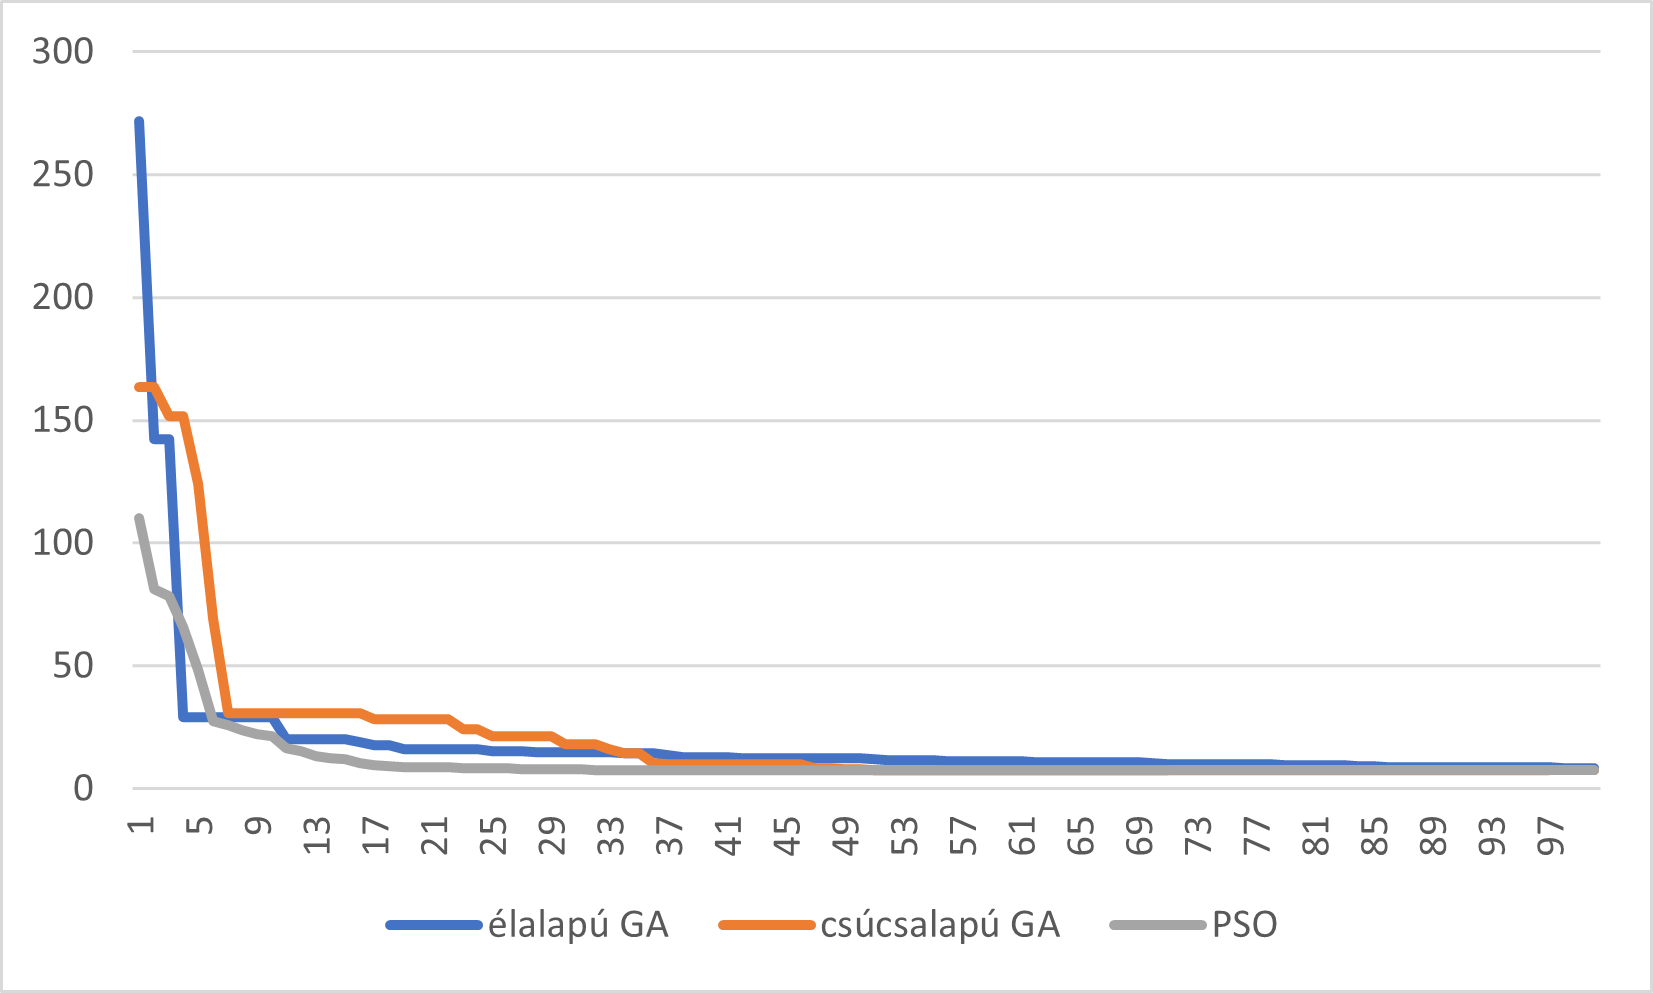
\includegraphics[width=0.30\linewidth]{25-8-20-cost}}
	\hspace{5pt}
	\subfigure[$H_{50,16,10}$]{
		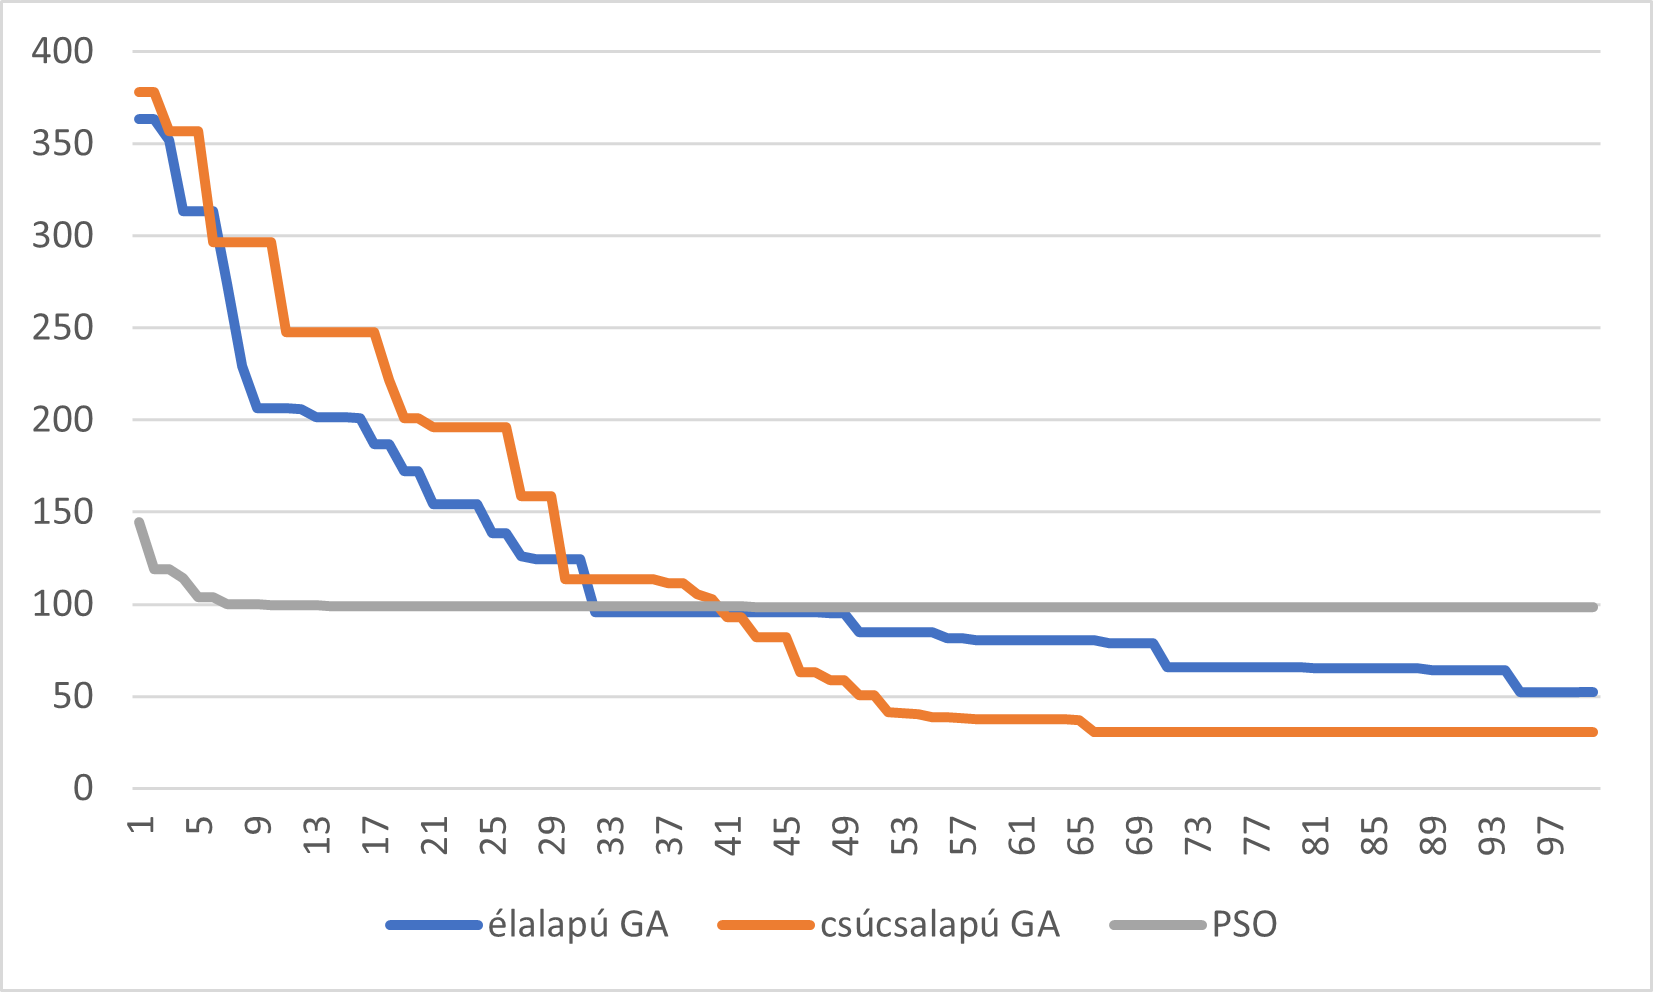
\includegraphics[width=0.30\linewidth]{50-16-10-cost}}
	\hspace{5pt}
	\subfigure[$H_{100,32,5}$]{
		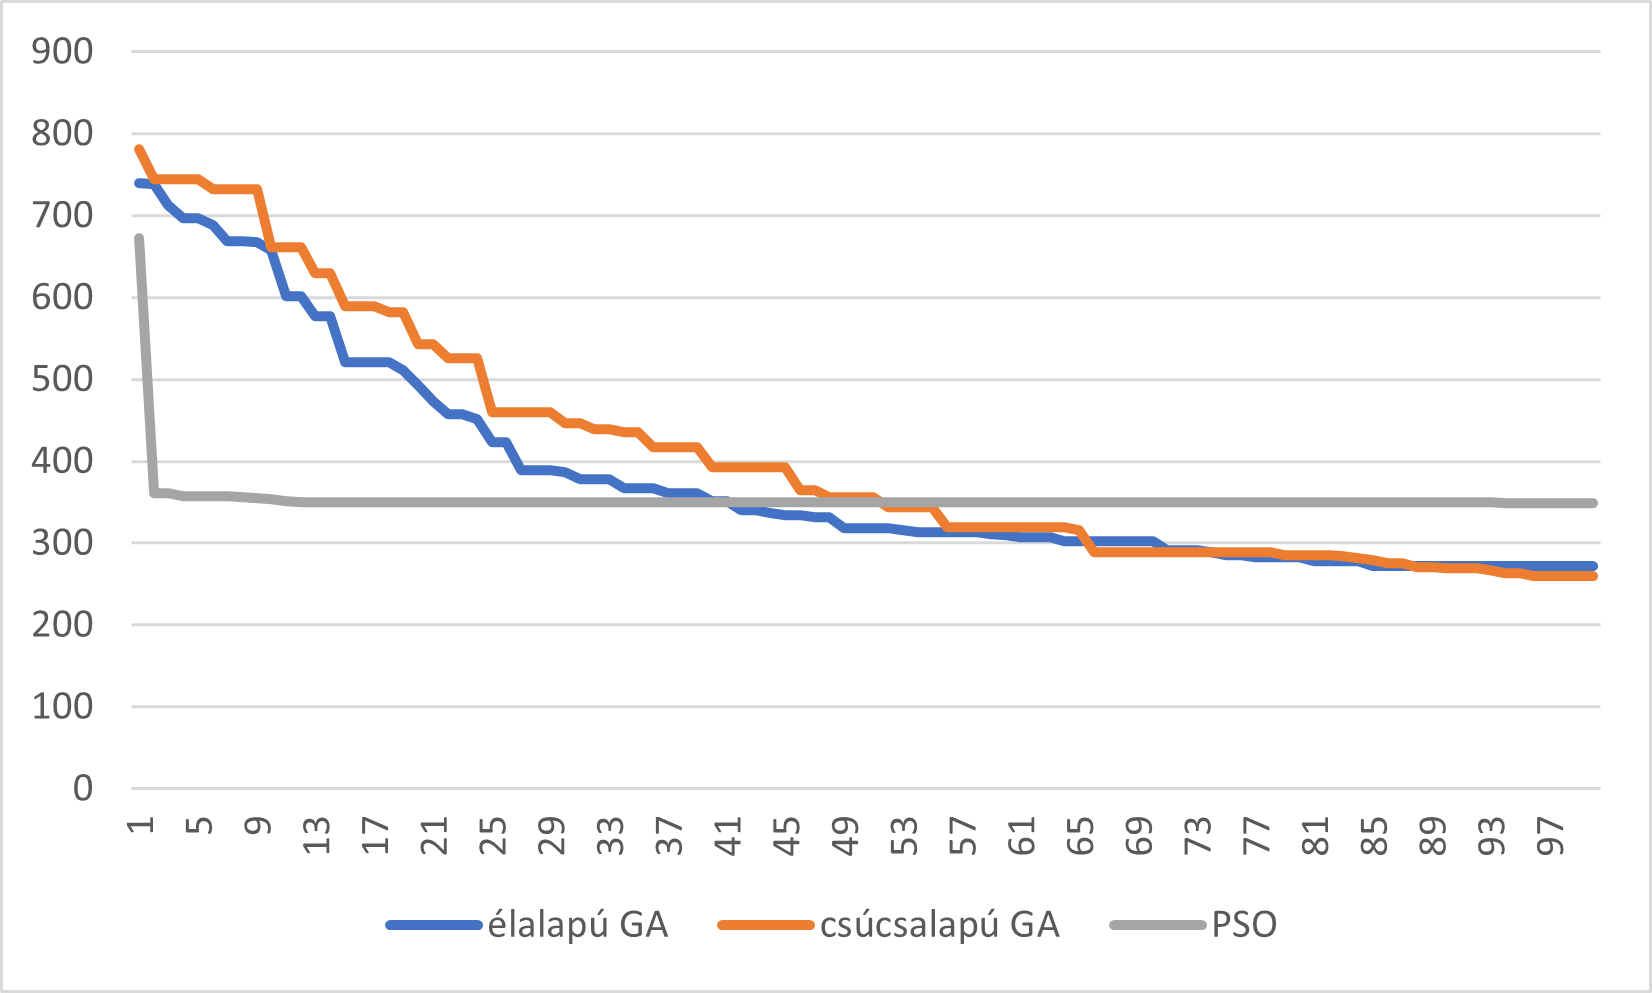
\includegraphics[width=0.30\linewidth]{100-32-5-cost}}
	\caption{Csúcs- és élszám együttes szám hatása a költségfüggvényre}
\end{figure}

Jól látható, hogy ekkor minden módszer teljesítménye romlik, azonban, míg a két GA hasonló ütemben konvergálni látszik, a PSO az optimalizáció elején megakad ennél a komplexitásnál.

\begin{figure}[H]
	\centering
	\subfigure[$H_{25,8,20}$]{
		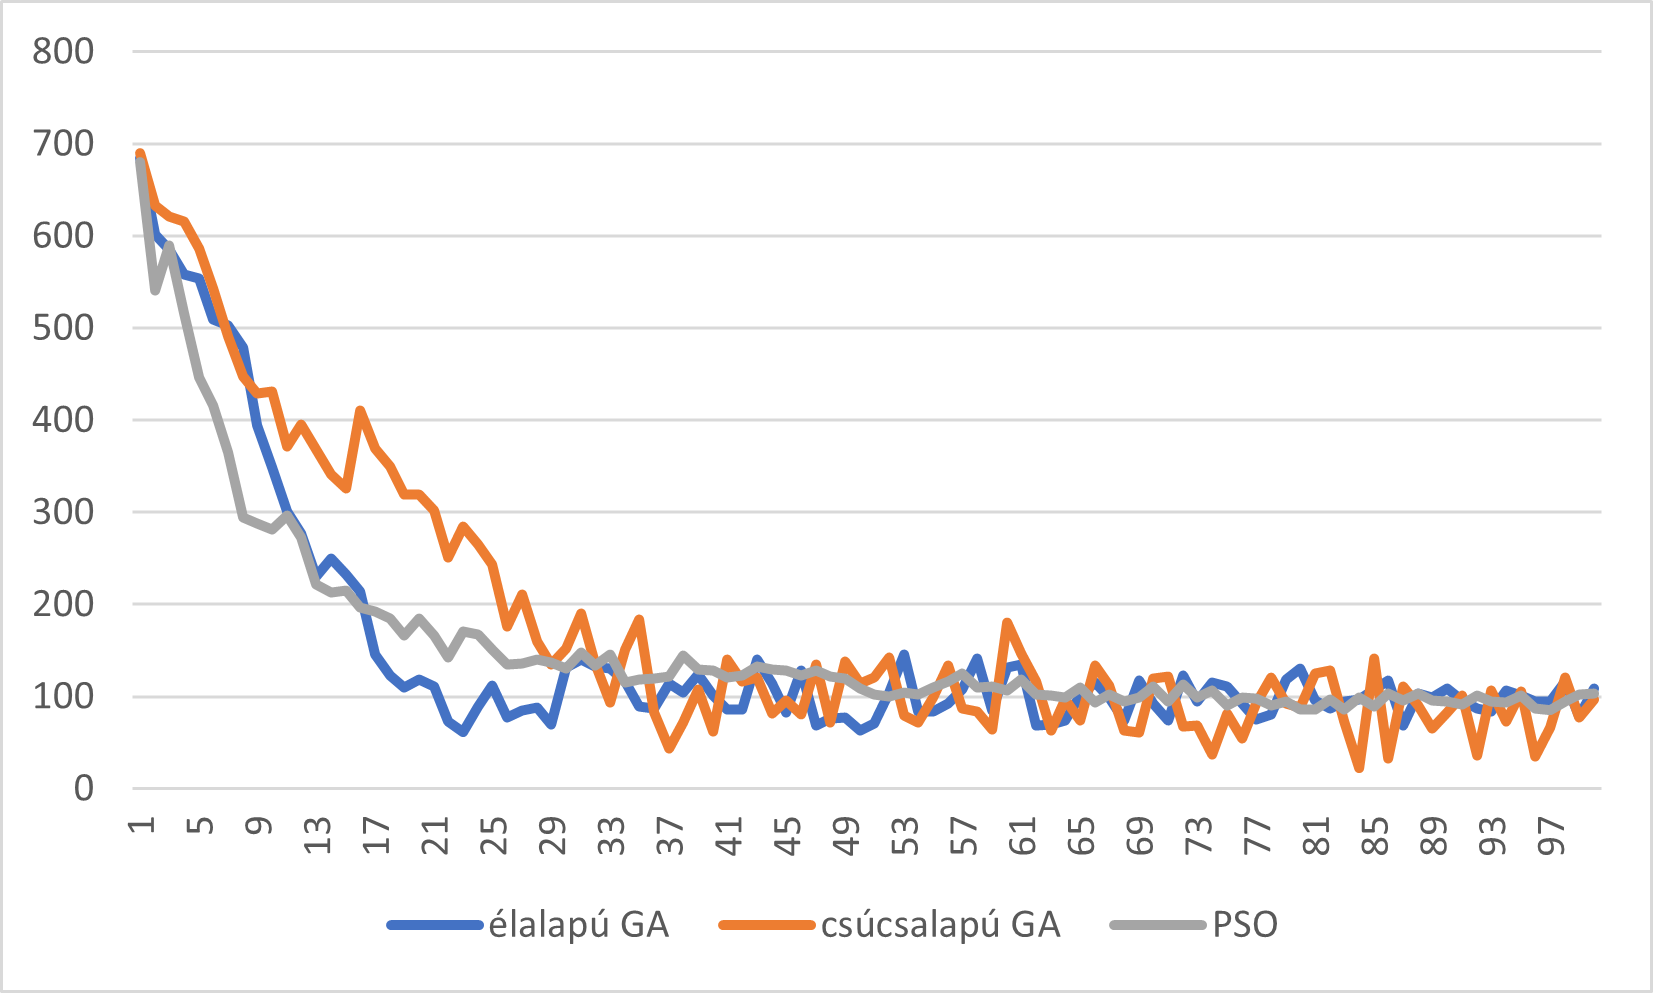
\includegraphics[width=0.30\linewidth]{25-8-20-cost-mean}}
	\hspace{5pt}
	\subfigure[$H_{50,16,10}$]{
		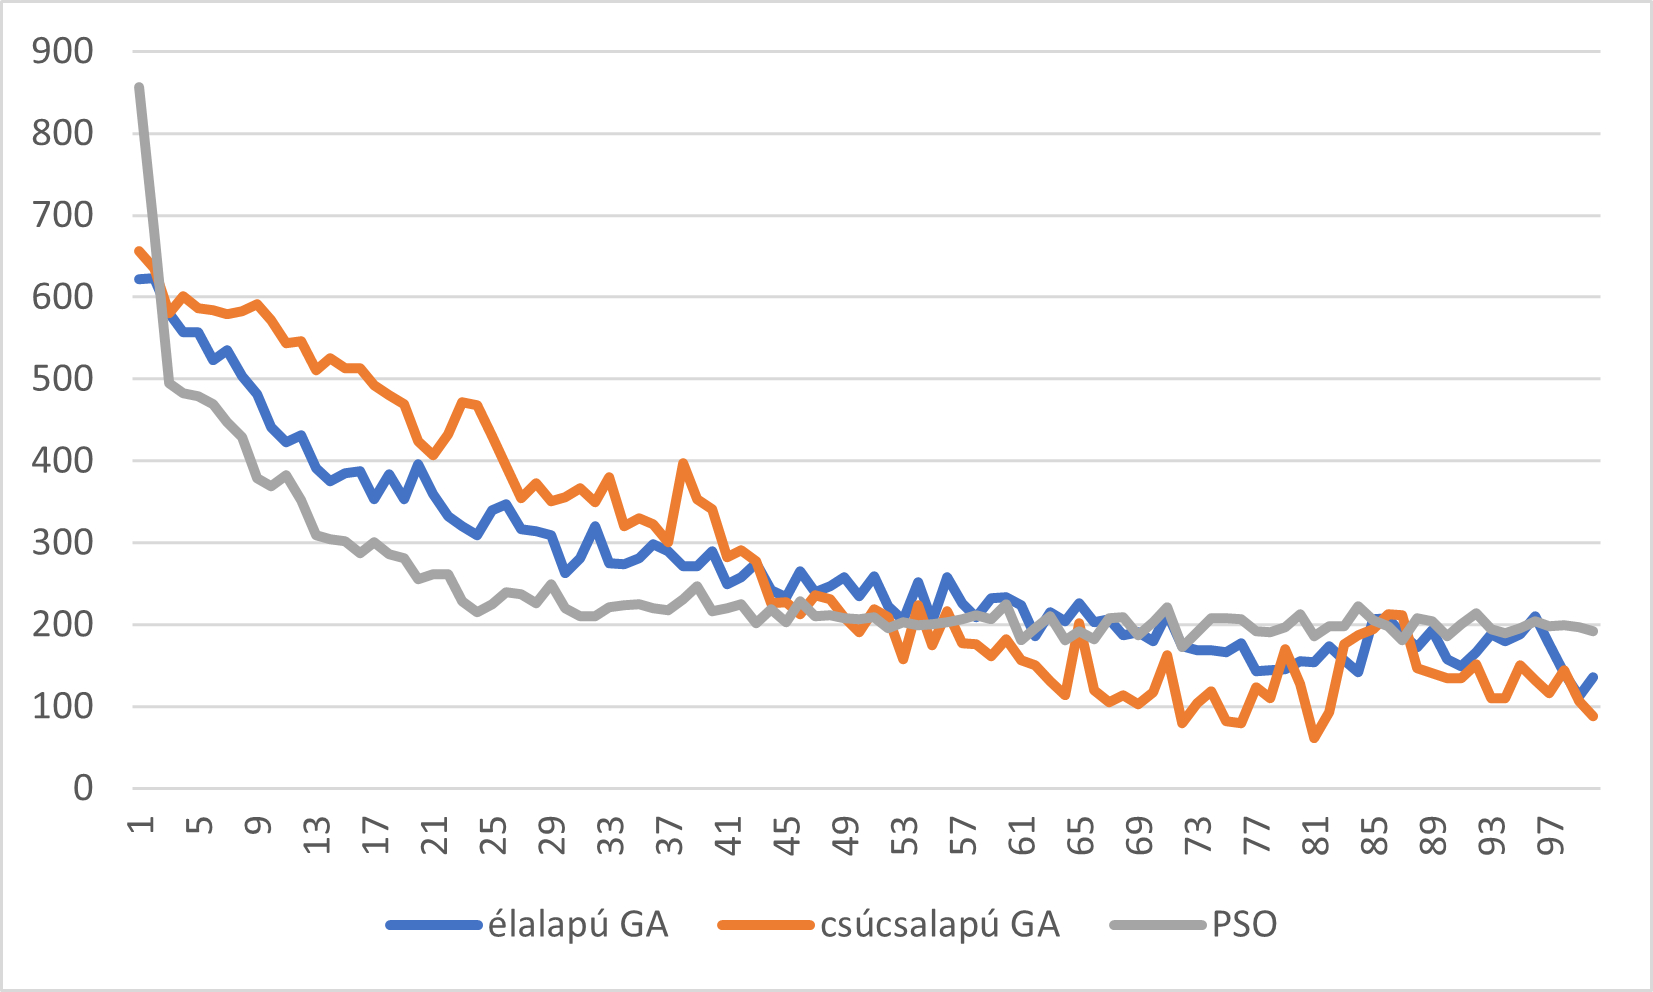
\includegraphics[width=0.30\linewidth]{50-16-10-cost-mean}}
	\hspace{5pt}
	\subfigure[$H_{100,32,5}$]{
		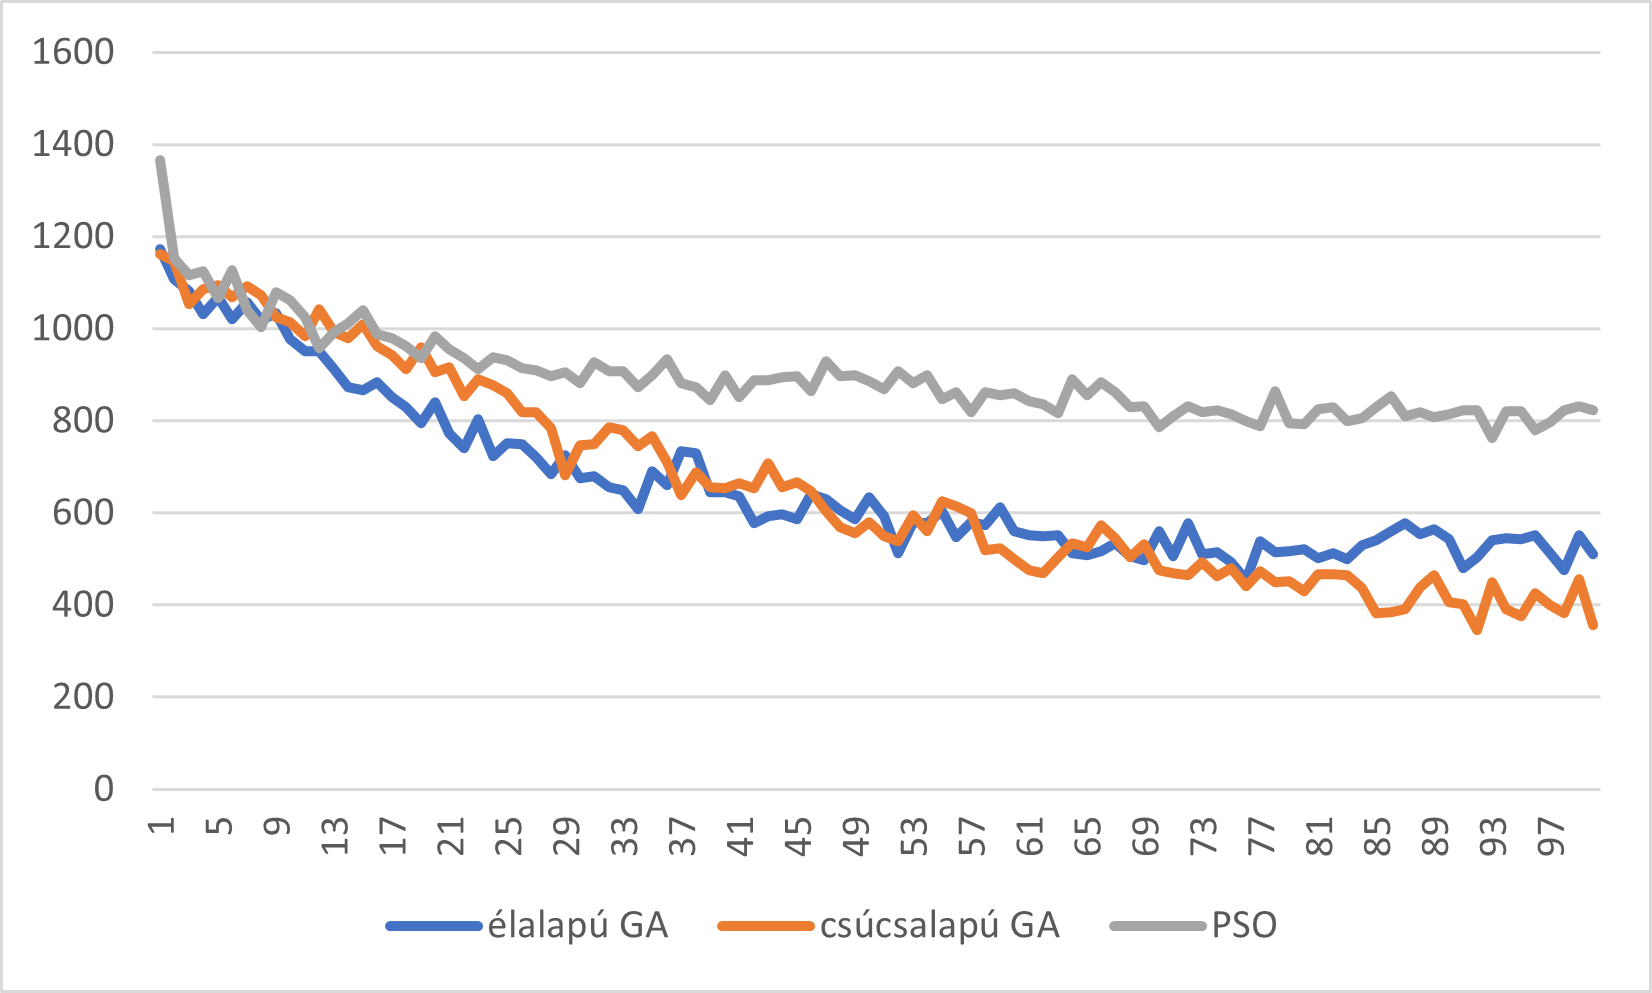
\includegraphics[width=0.30\linewidth]{100-32-5-cost-mean}}
	\caption{Csúcs- és élszám együttes hatása a megoldáspopuláció költségfüggvényének átlagára}
\end{figure}

Az átlagértéket vizsgálva is azt állapíthatjuk meg, hogy a PSO a $H_{100,32,20}$ esetében már jóval elmarad a másik két módszer mögött. Érdekes összehasonlítani a GA módszereket a kizárólag éleket változtató kísérlettel; 50 csúcs esetén ugyanis jobban teljesítenek, de 100-nál már feltűnően rosszabbul. Kérdéses, hogy ez a komplexitás növekedése miatt van vagy a véletlen hipergráfok harmadik paramétere miatt. 

\subsubsection{Sűrűség növelése}

Eddig a véletlen hipergráfok minden paraméterét vizsgáltuk, kivéve az élek tartalmazási valószínűségét, amelyet a hipergráf sűrűségeként is értelmezhetünk. A következő kísérletben a $H_(25,8,20)$, $H_(25,8,40)$ és $H_(25,8,60)$ hipergráfokon keresztül ezek hatását láthatjuk.

\begin{figure}[H]
	\centering
	\subfigure[$H_{25,8,20}$]{
		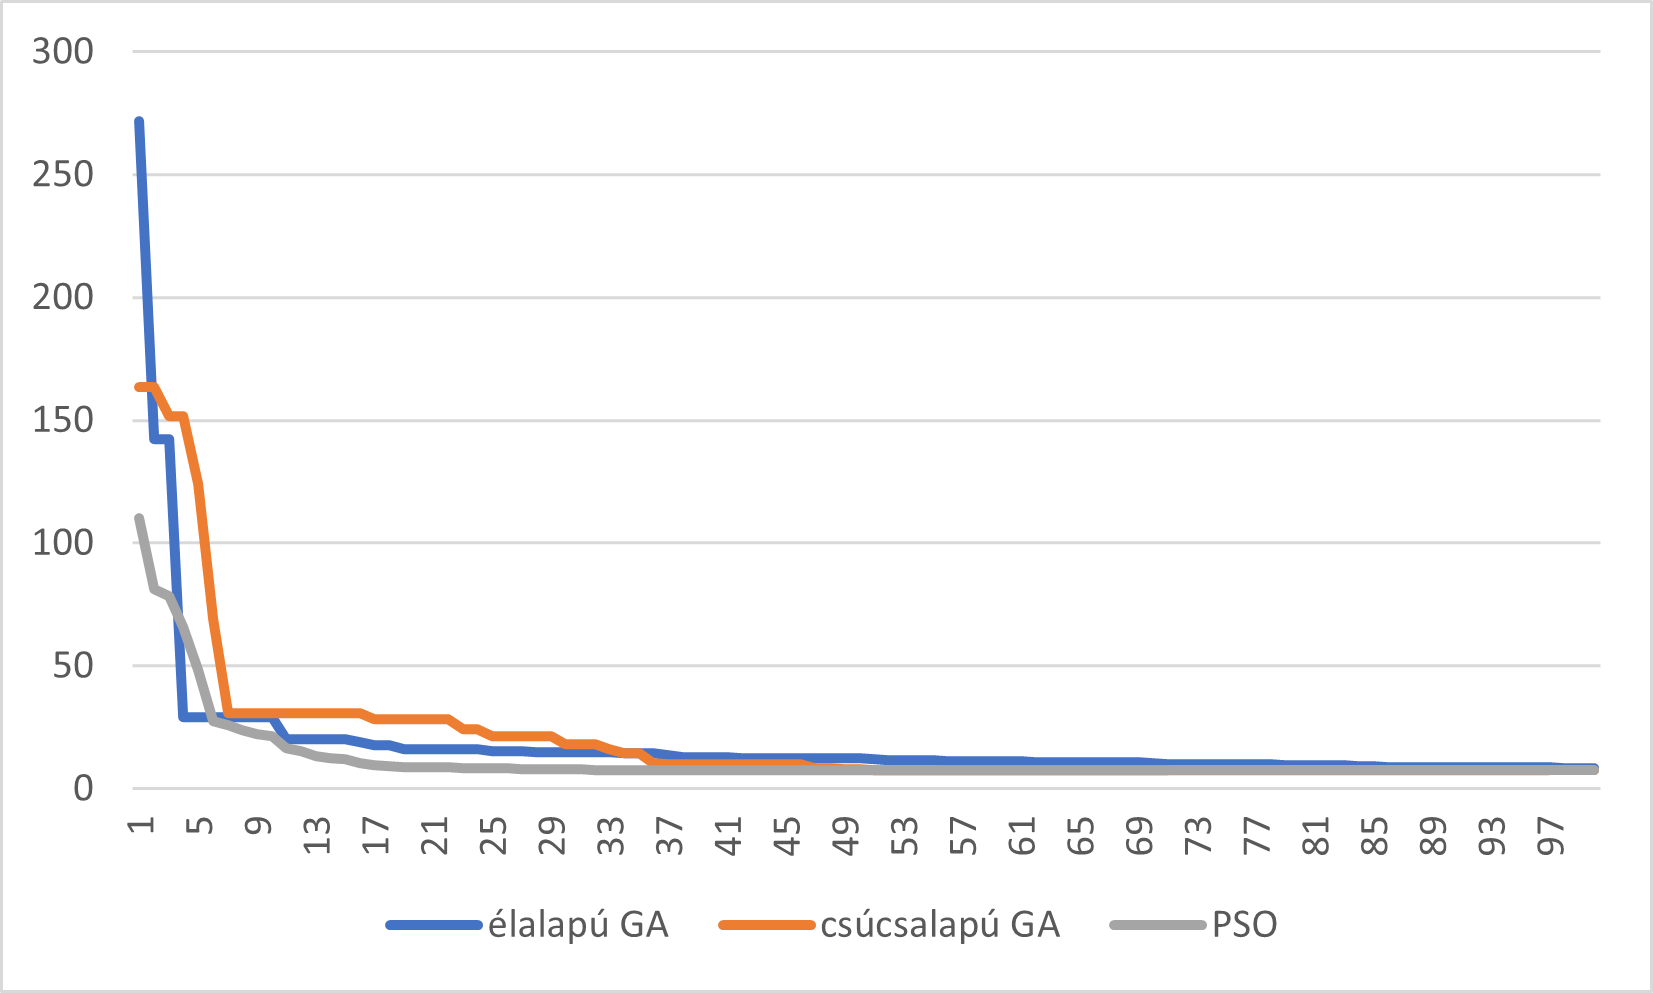
\includegraphics[width=0.30\linewidth]{25-8-20-cost}}
	\hspace{5pt}
	\subfigure[$H_{25,8,40}$]{
		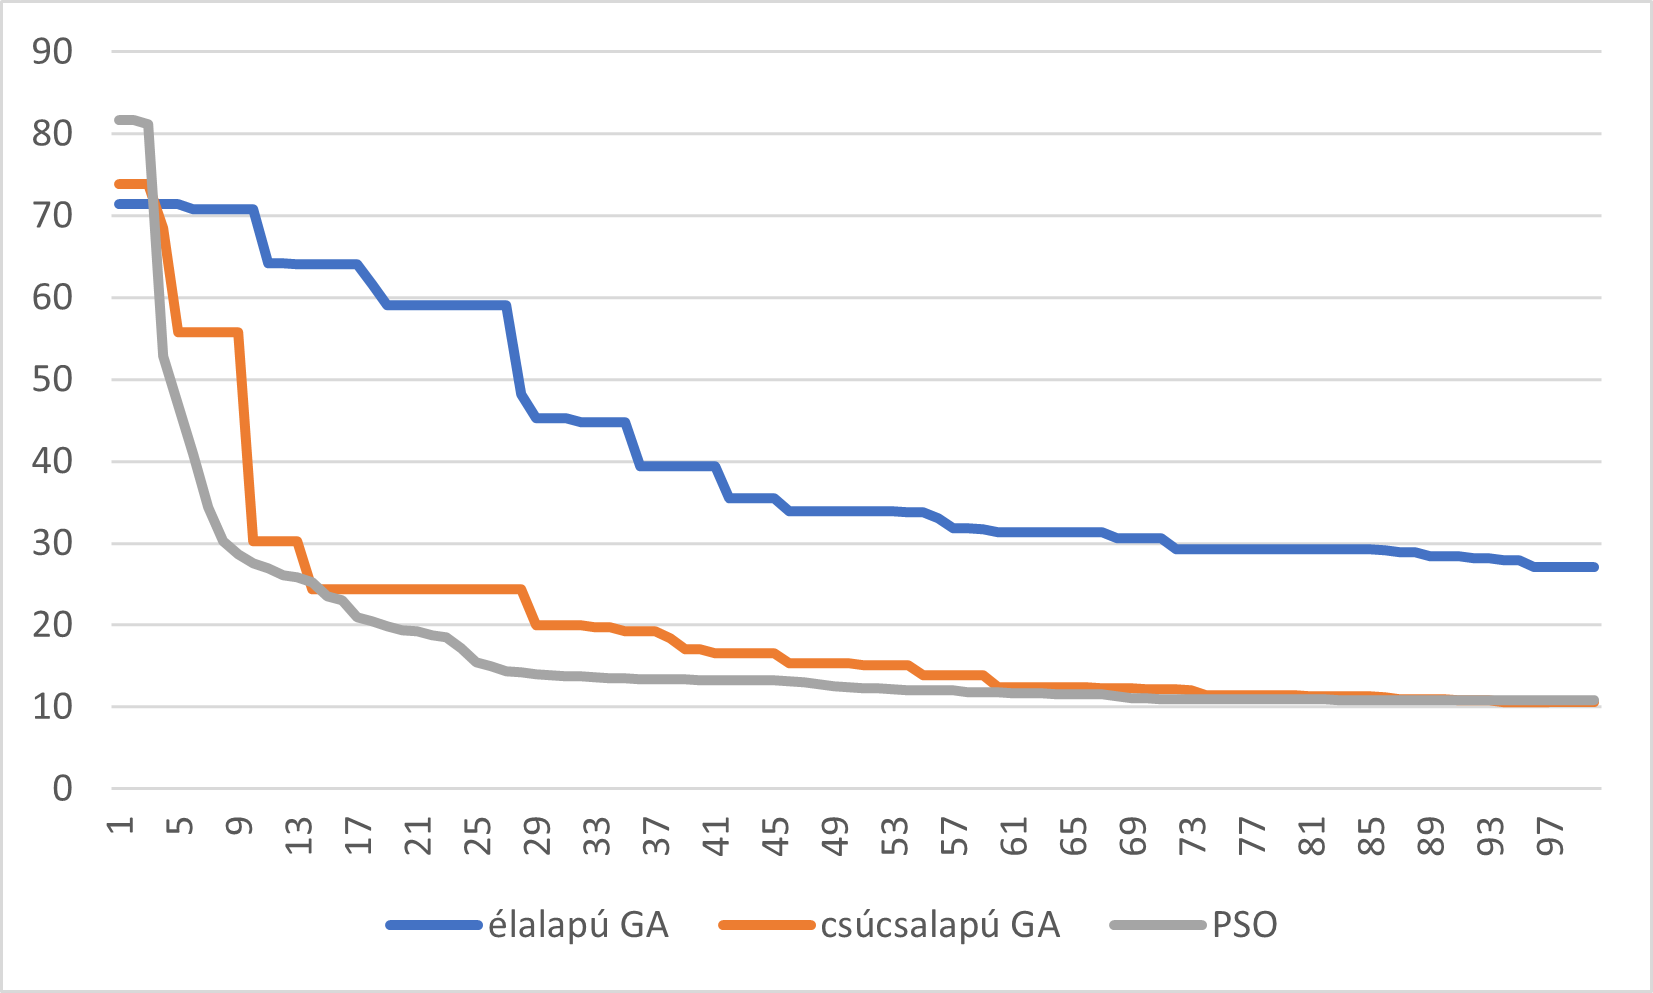
\includegraphics[width=0.30\linewidth]{25-8-40-cost}}
	\hspace{5pt}
	\subfigure[$H_{25,8,60}$]{
		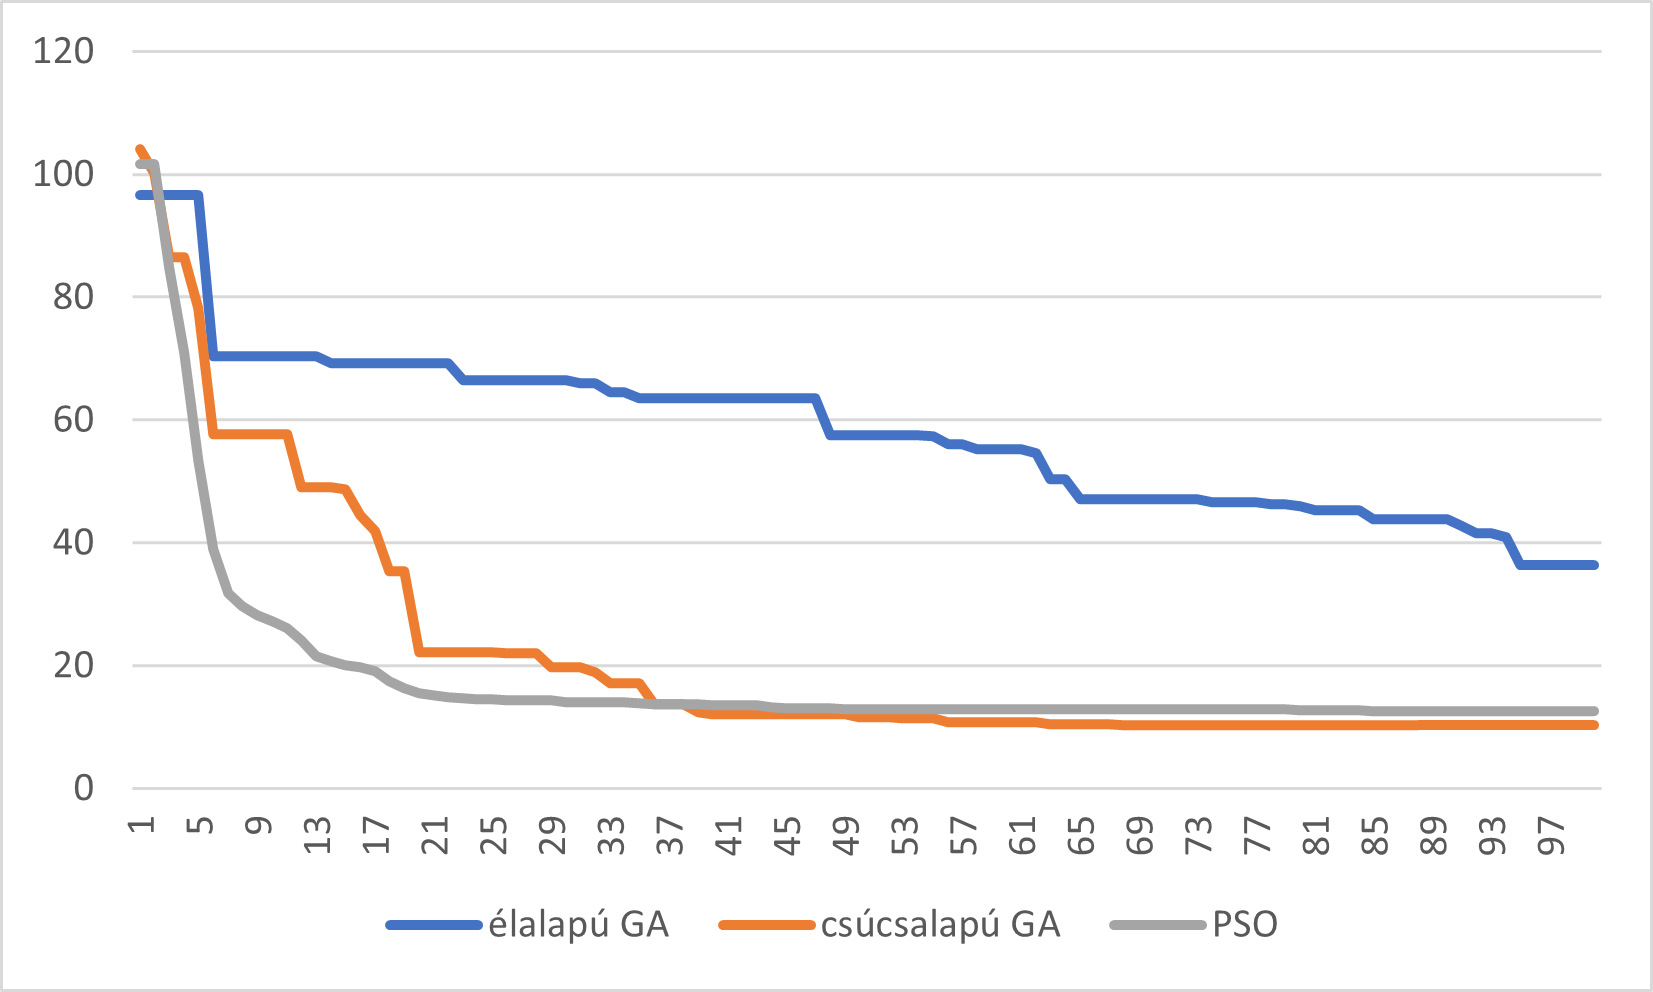
\includegraphics[width=0.30\linewidth]{25-8-60-cost}}
	\caption{Sűrűség hatása a költségfüggvényre}
\end{figure}

Bár a csúcsalapú GA és a PSO hasonlóan teljesít ennek a paraméternek a változtatása során, az élalapú GA teljesítményét láthatóan nagyban rontja. Elképzelhető, hogy ekkora sűrűségek mellett már negatív hatása van annak, hogy az új megoldások mindkét szülőtől fele-fele arányban öröklik a géneket.

% TODO konklúzió : öröklődés fele-fele arányban az élGA-nél

\subsection{Algoritmusok hatékony paraméterezésére}

% TODO grid search a paramétereken

\subsubsection{Iterációk száma kontra megoldáspopuláció mérete}


\subsection{Előnyös inicializálási módszerek}

Optimalizációs algoritmusok során létrehozandó új megoldások generálására három különböző módszert vezettem be; az egyenletes eloszláson, éleken, illetve erőalapú gráfelrendezésen alapulót. Felmerül a kérdés, hogy melyik milyen gyors konvergenciához vezet, továbbá milyen költségfüggvény érhető el a használatukkal. Mint a \ref{initialization_d} alfejezetben említettem, a konkrét módszerek főként a csúcsonkénti $x$ és $y$ koordináták pozicionálására fókuszálnak, a $d$ értékek háttérbe szorulnak. Ennek ellensúlyozására a $d$ értékek meghatározása véletlenszerűen, de az adott csúcs élszomszédainak távolságstatisztikái alapján is meghatározhatók. Ezen kísérletek során végig a $H_{25,8,20}$-at használom.

\subsubsection{Véletlenszerű $d$ értékek}

Az előbbi esetben az figyelhető meg, hogy a különböző módszerek végül mind hasonlóan jó költségfüggvényt képesek elérni, a 7.4-8.5 sávban. Az egyedüli kivételt a PSO/élalapú inicializálás képezi, amely egy nagyságrenddel elmarad ettől. Érdemes megfigyelni, hogy a konvergencia sokkal gyorsabb az erőalapú módszer esetén, ahol már az első iteráció során az elért optimumhoz közel kerülünk, azonban egyedül az élalapú GA tűnik képesnek fenntartható konvergenciára.

\begin{figure}[H]
	\centering
	\subfigure[Véletlen inicializálás]{
		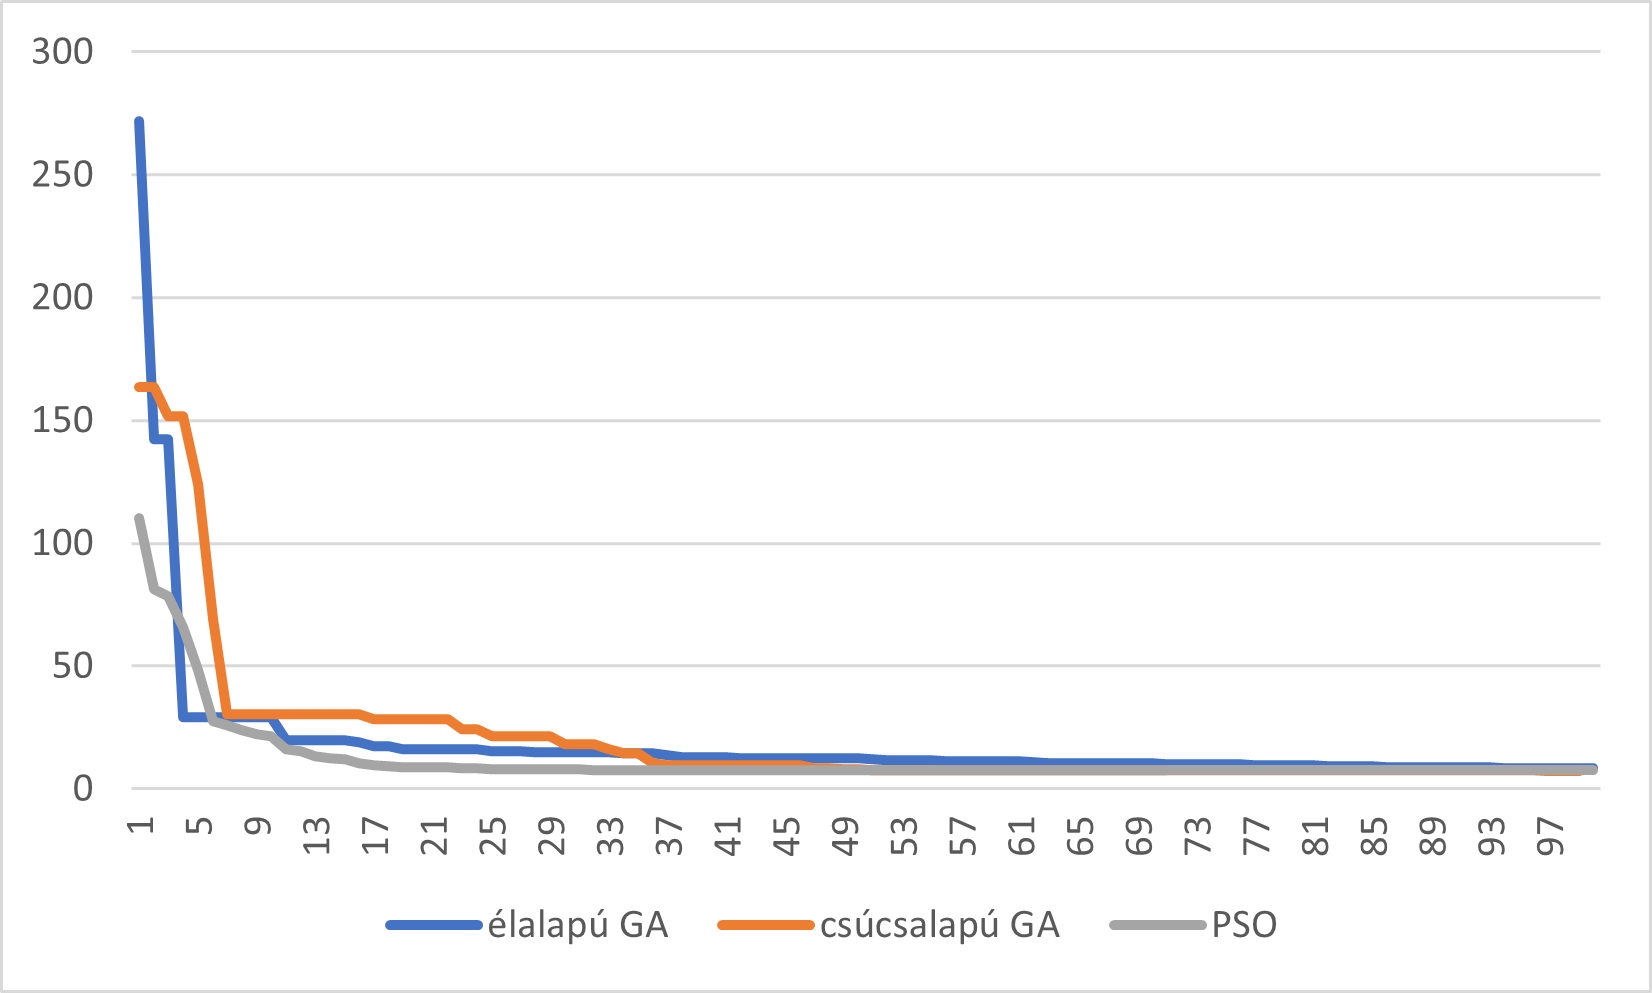
\includegraphics[width=0.30\linewidth]{init-rand-none-cost}}
	\hspace{5pt}
	\subfigure[Élalapú inicializálás]{
		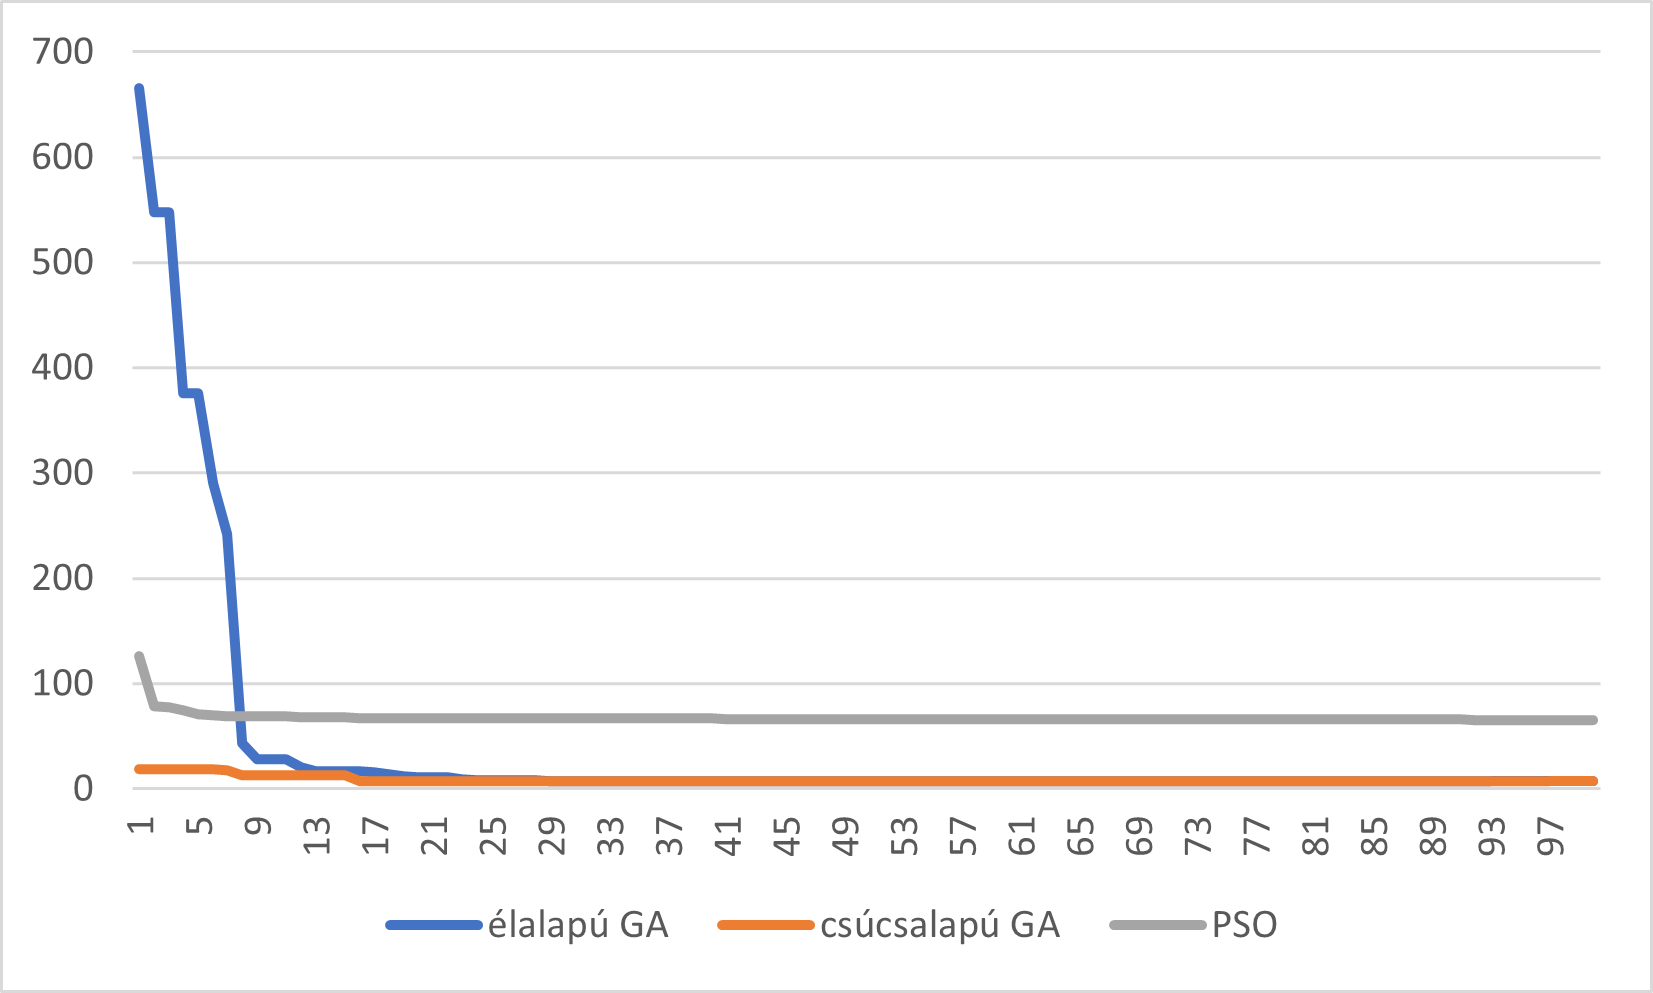
\includegraphics[width=0.30\linewidth]{init-edge-none-cost}}
	\hspace{5pt}
	\subfigure[Erőalapú inicializálás]{
		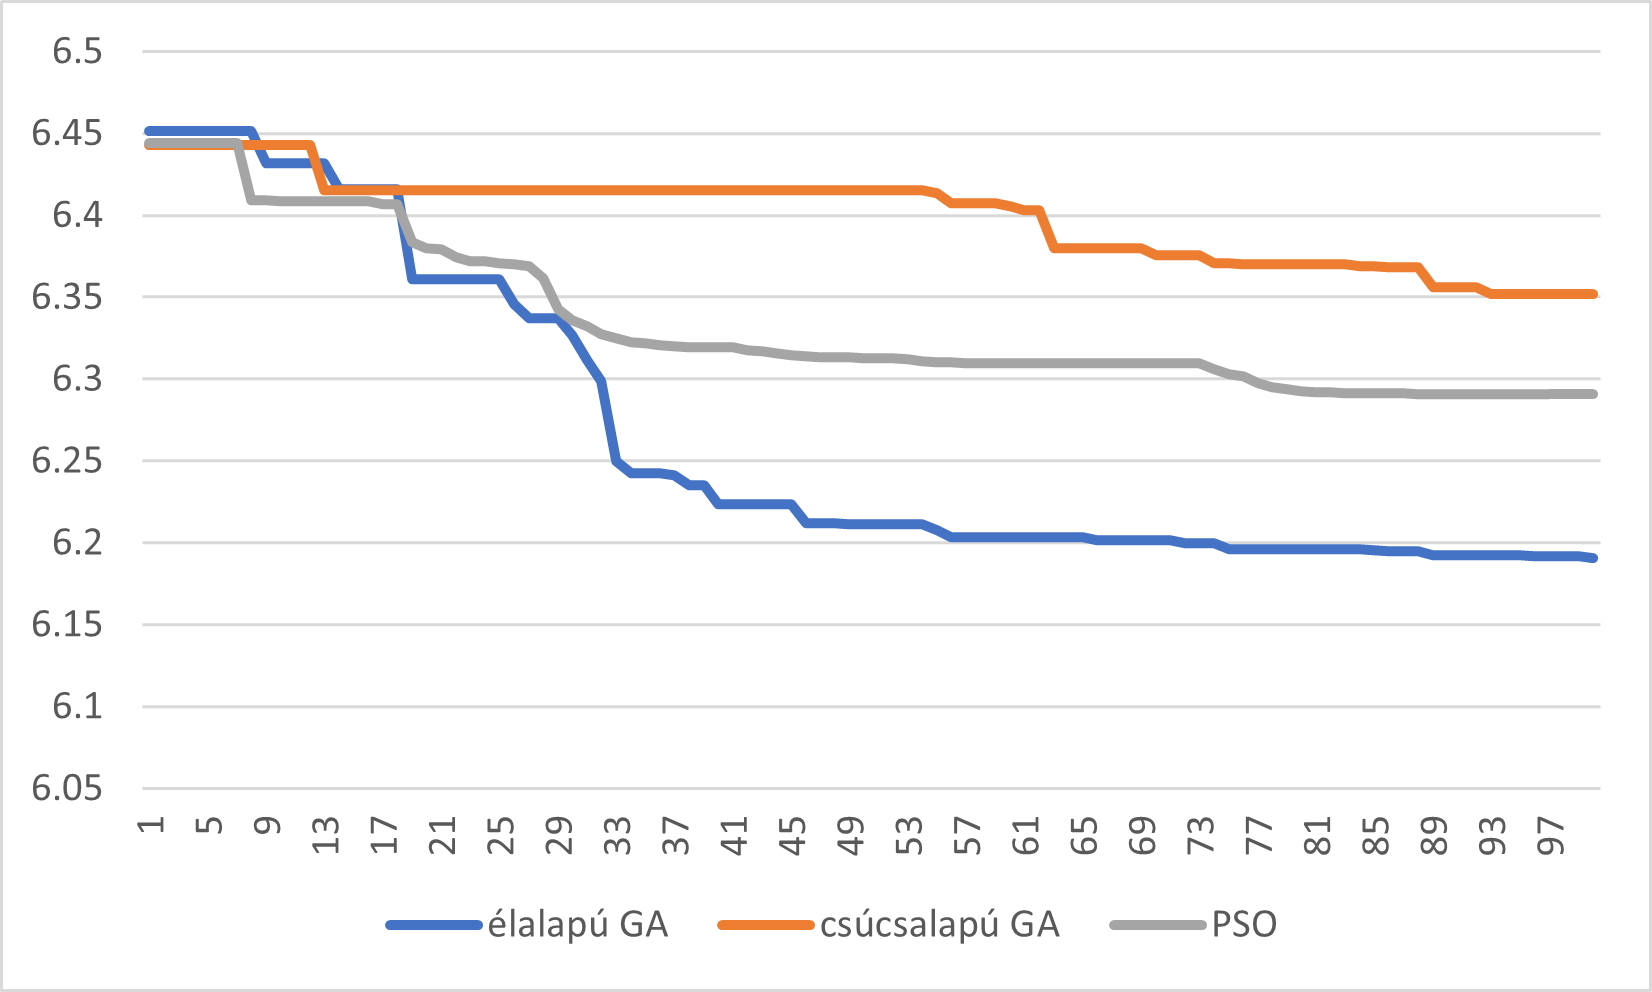
\includegraphics[width=0.30\linewidth]{init-spring-none-cost}}
	\caption{Inicializálás véletlen $d$ értékekkel - költségfüggvények}
\end{figure}

Megerősíti a korábbi megfigyeléseket a megoldáspopuláció átlagainak vizsgálata is, amely során azt láthatjuk, hogy a PSO átlaga elmarad a többitől mind az élalapú, mind az erőalapú megoldás esetén, míg az utóbbinál egyedül az élalapú GA tud javítani a kezdeti értékén.

\begin{figure}[H]
	\centering
	\subfigure[Véletlen inicializálás]{
		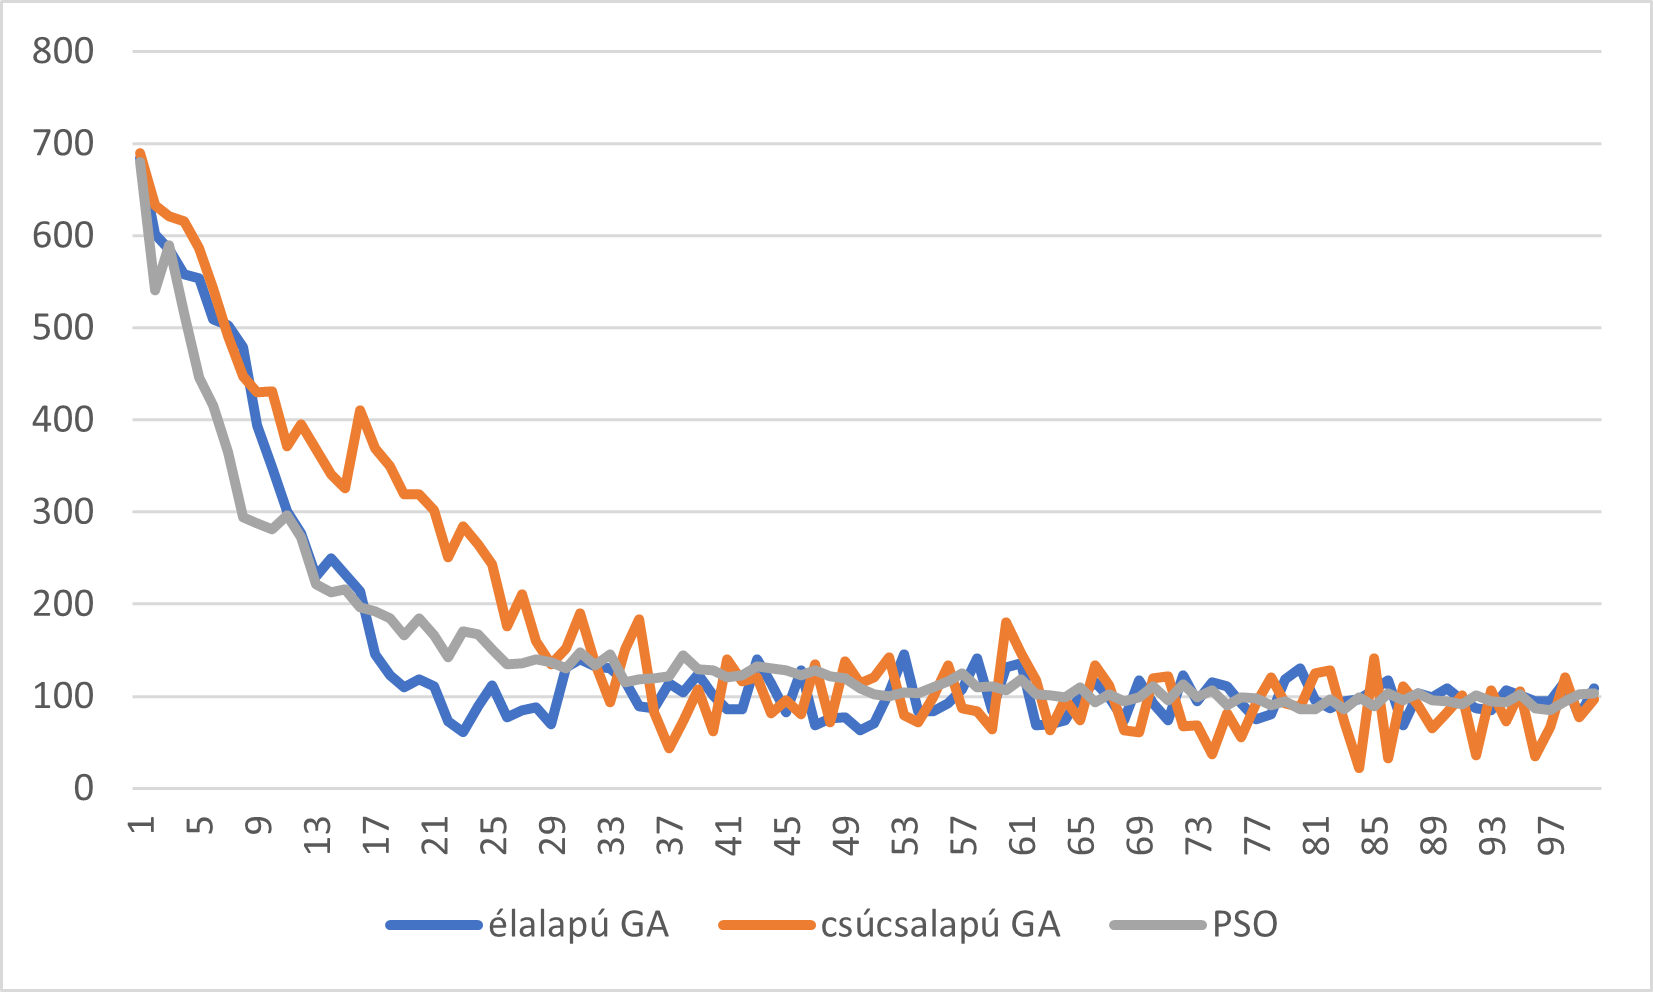
\includegraphics[width=0.30\linewidth]{init-rand-none-cost-mean}}
	\hspace{5pt}
	\subfigure[Élalapú inicializálás]{
		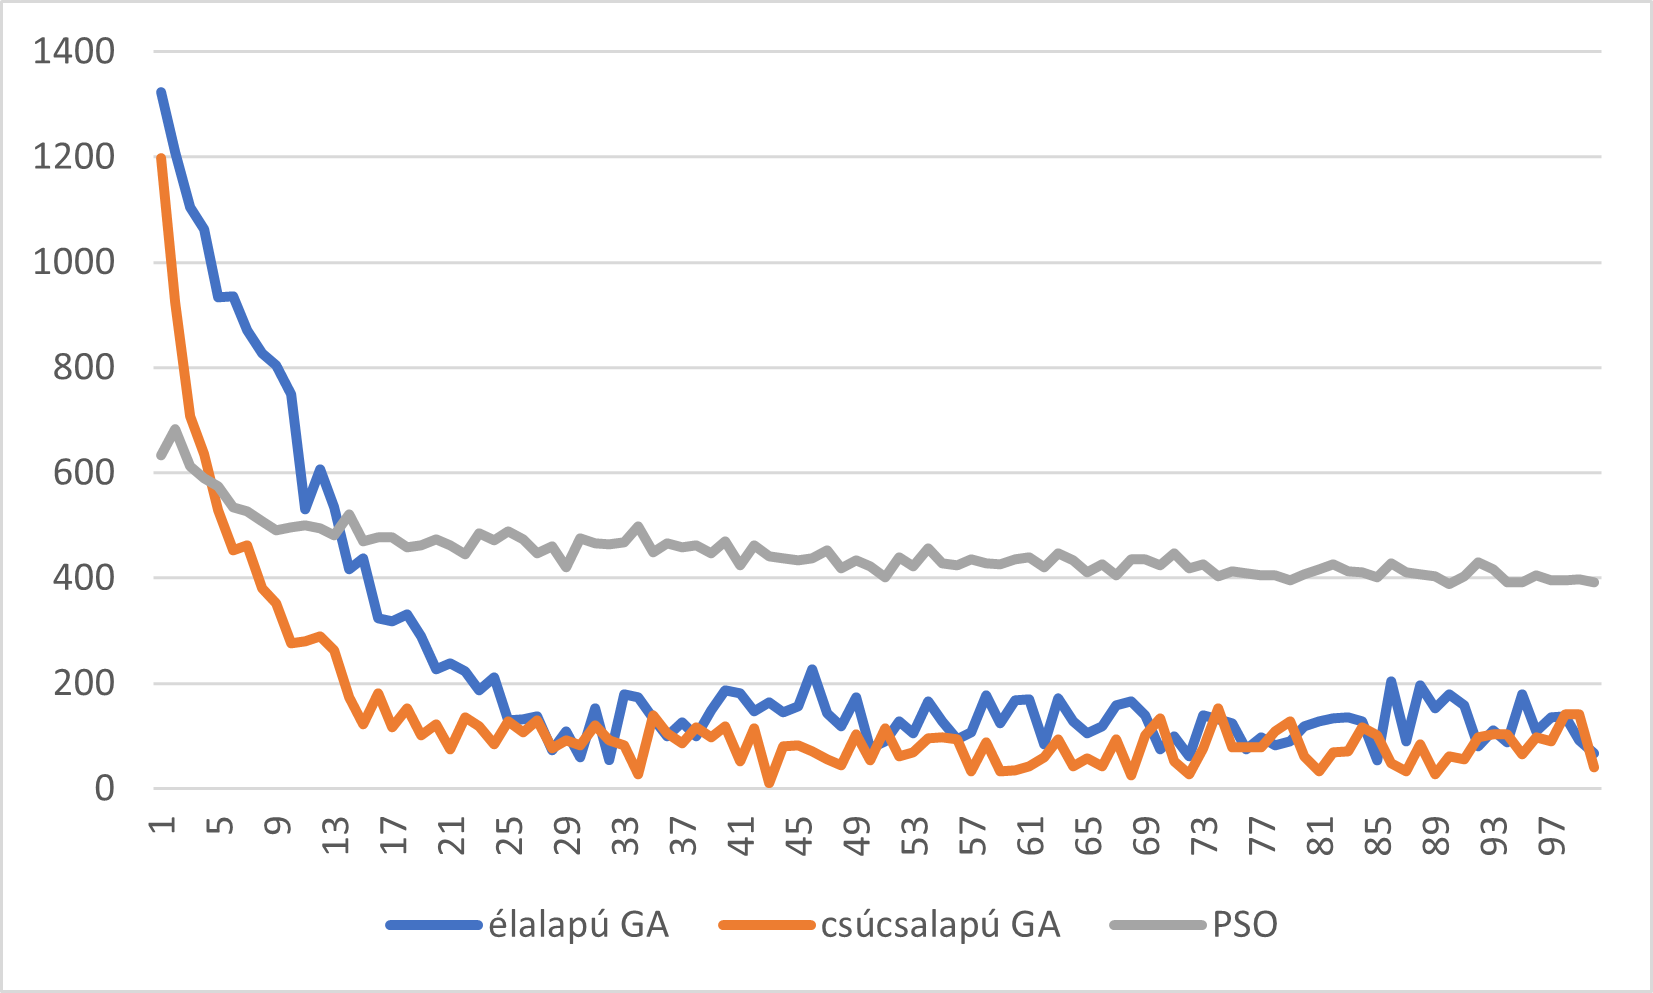
\includegraphics[width=0.30\linewidth]{init-edge-none-cost-mean}}
	\hspace{5pt}
	\subfigure[Erőalapú inicializálás]{
		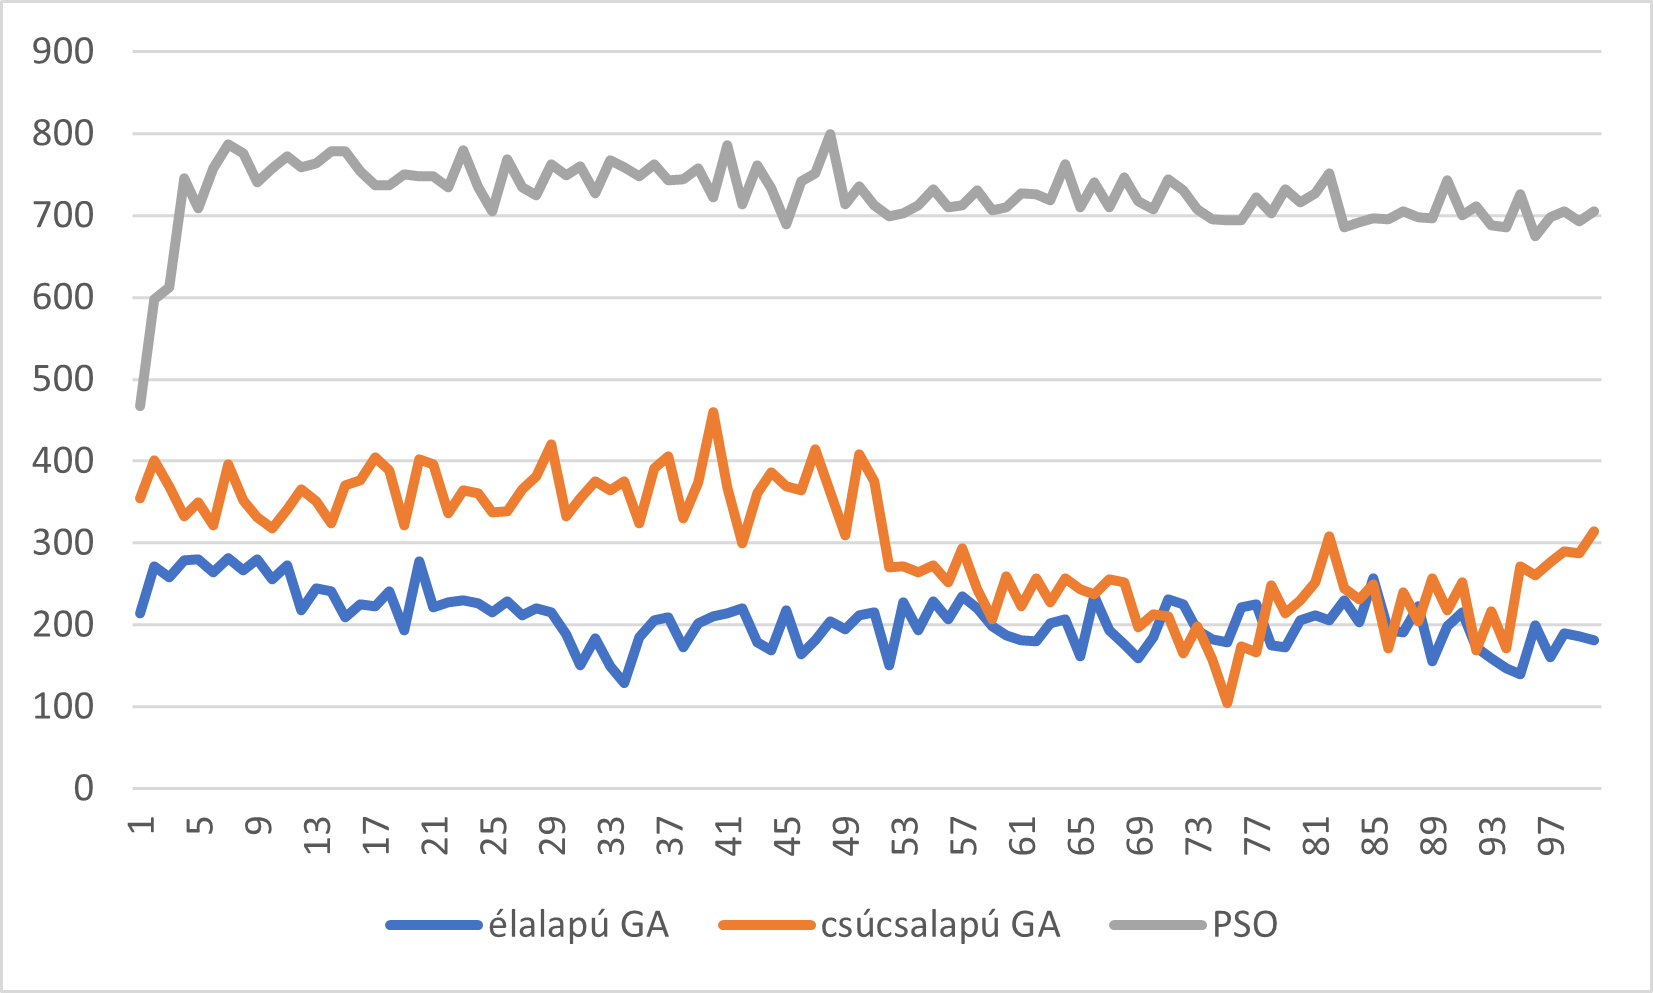
\includegraphics[width=0.30\linewidth]{init-spring-none-cost-mean}}
	\caption{Inicializálás véletlen $d$ értékekkel - költségfüggvények átlaga}
\end{figure}

\subsubsection{Statisztikák a $d$ paraméteren}

Fontos kiemelni, hogy a vizsgált hipergráf esetén az optimális kirajzolás élenként egy szegmenst használ (hiszen 8 halmazig minden hipergráf síkbarajzolható), így a maximum érték kiválasztása egyben a legjobb is kell legyen. Mivel ez több halmaz esetén nem feltétlenül igaz, ezért kérdéses, hogy a szegmensek kialakításához szükséges egyéb stratégiákat ellen tudják-e a súlyozni az egyes algoritmusok.

\begin{figure}[H]
	\centering
	\subfigure[Véletlen inicializálás]{
		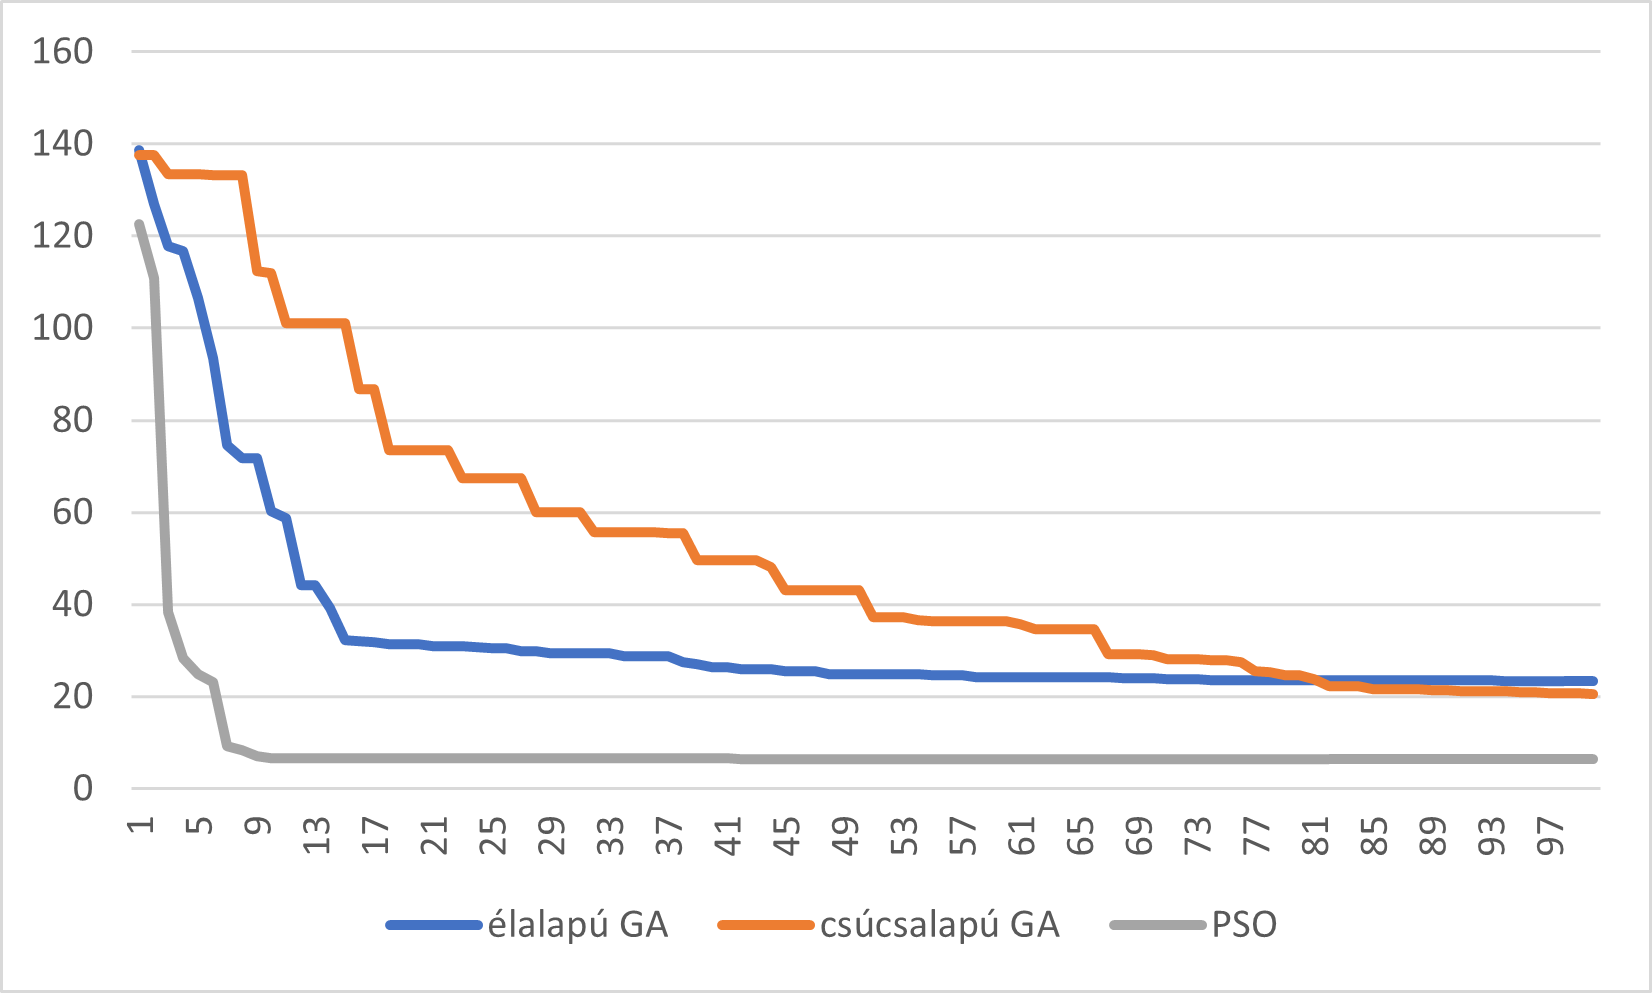
\includegraphics[width=0.30\linewidth]{init-rand-min-cost}}
	\hspace{5pt}
	\subfigure[Élalapú inicializálás]{
		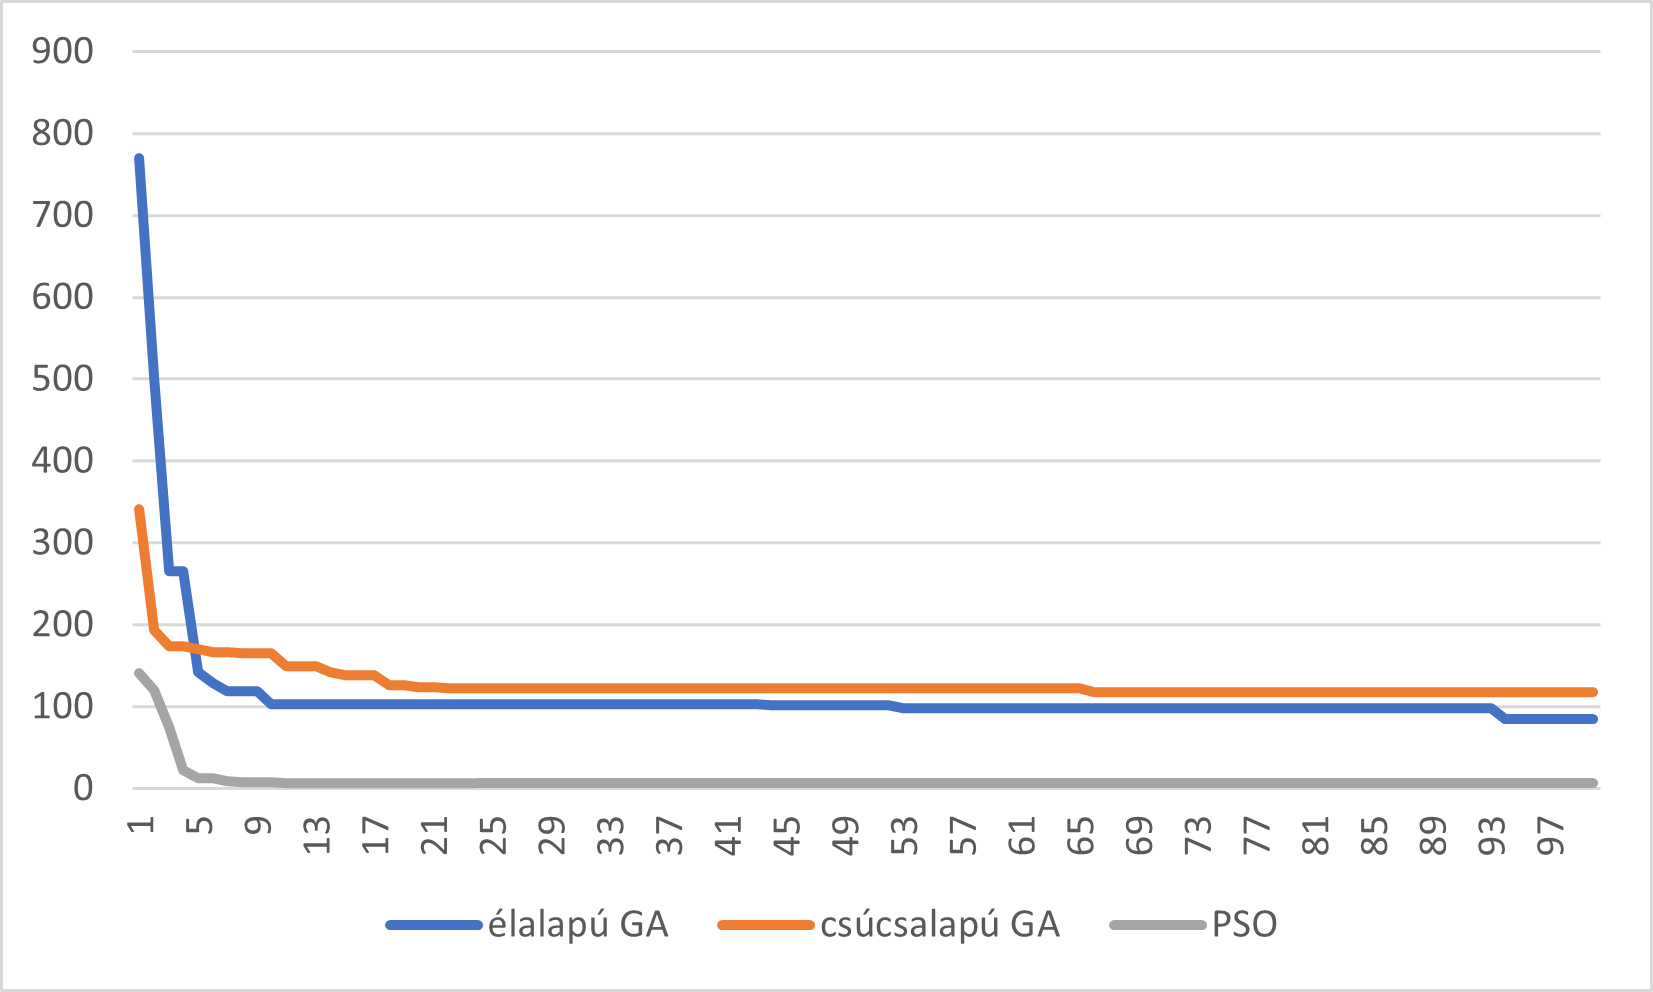
\includegraphics[width=0.30\linewidth]{init-edge-min-cost}}
	\hspace{5pt}
	\subfigure[Erőalapú inicializálás]{
		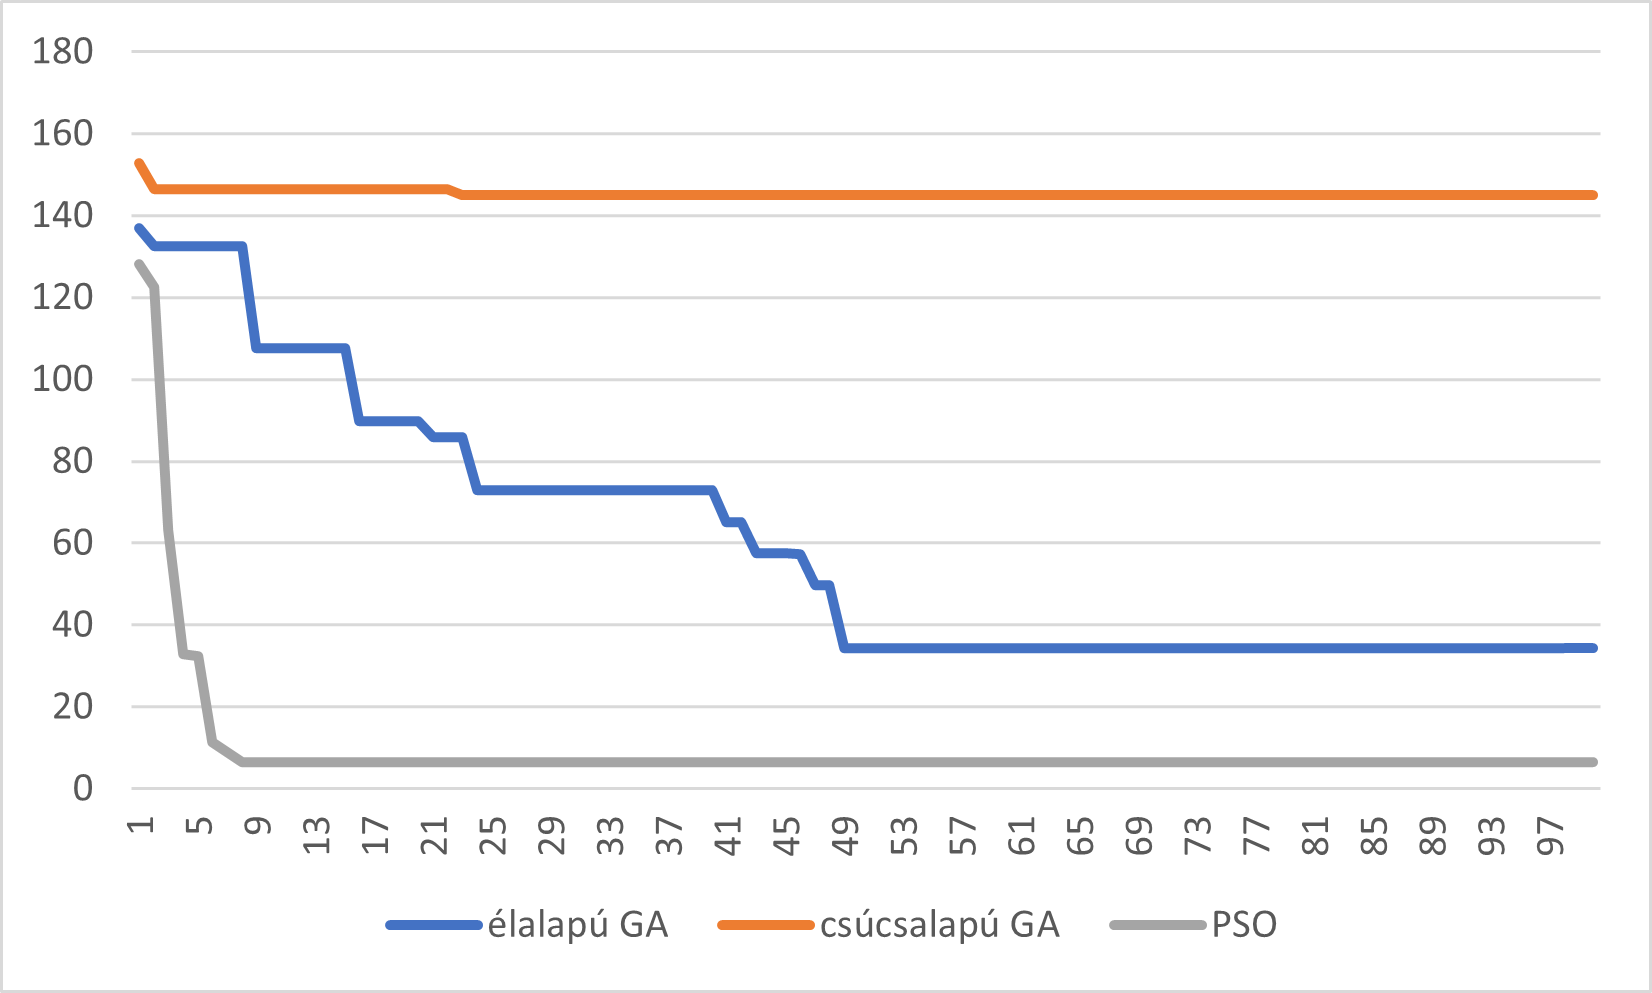
\includegraphics[width=0.30\linewidth]{init-spring-min-cost}}
	\subfigure[Véletlen inicializálás]{
		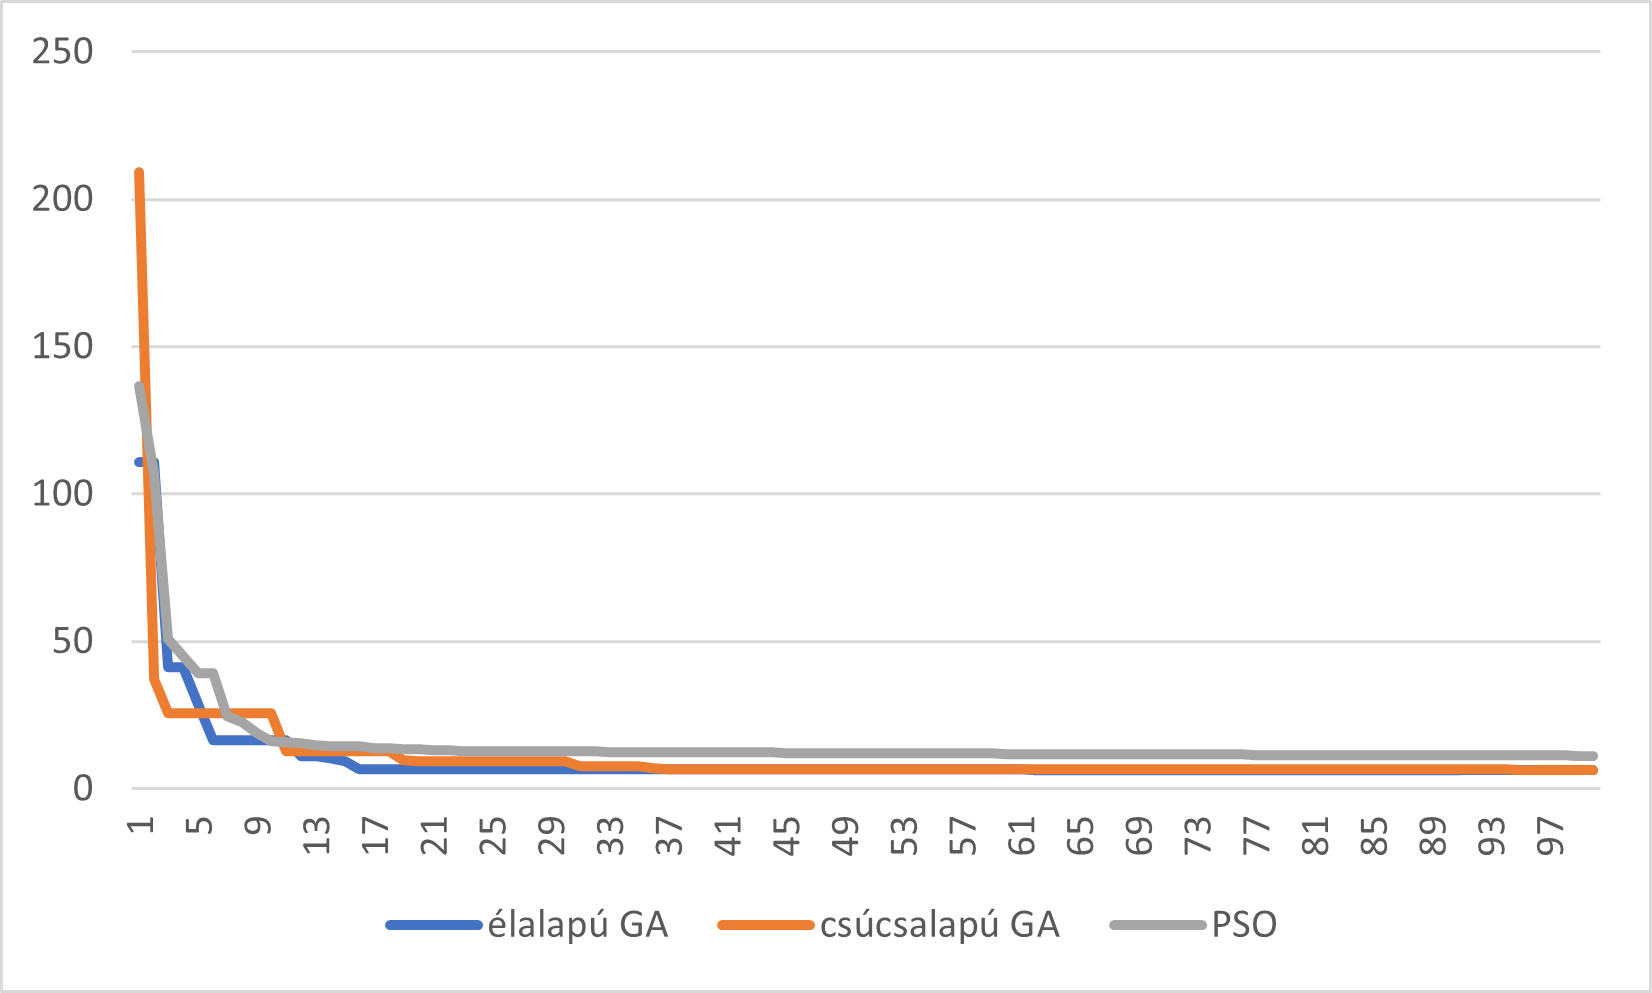
\includegraphics[width=0.30\linewidth]{init-rand-max-cost}}
	\hspace{5pt}
	\subfigure[Élalapú inicializálás]{
		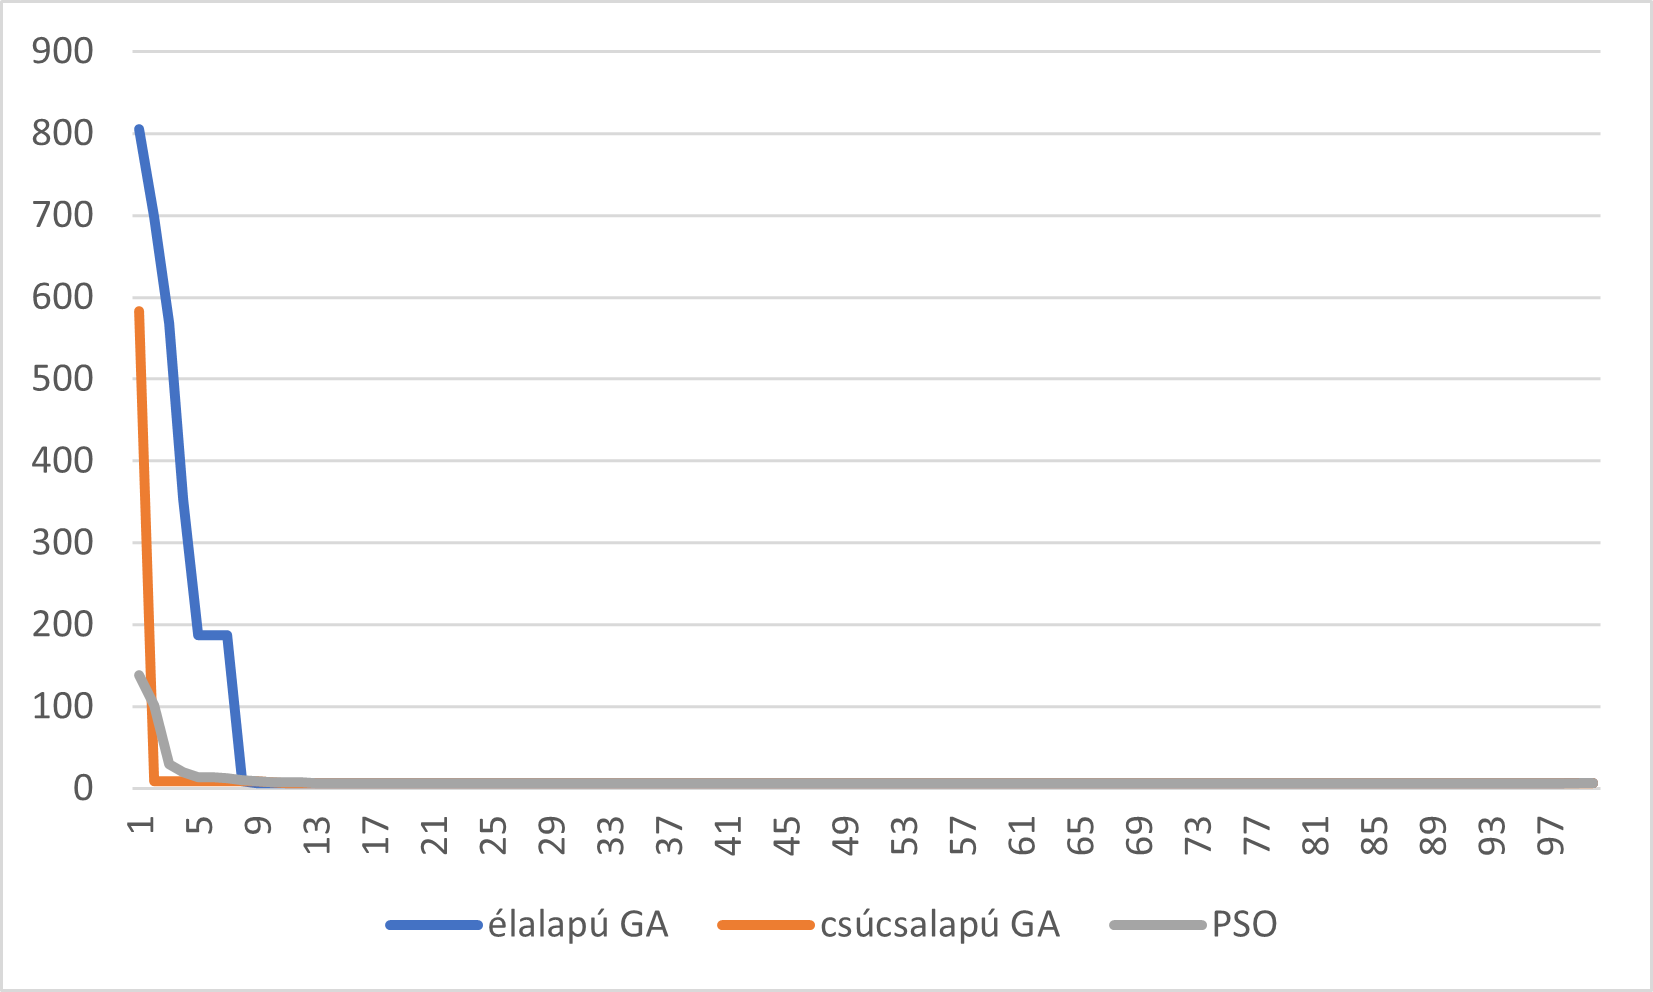
\includegraphics[width=0.30\linewidth]{init-edge-max-cost}}
	\hspace{5pt}
	\subfigure[Erőalapú inicializálás]{
		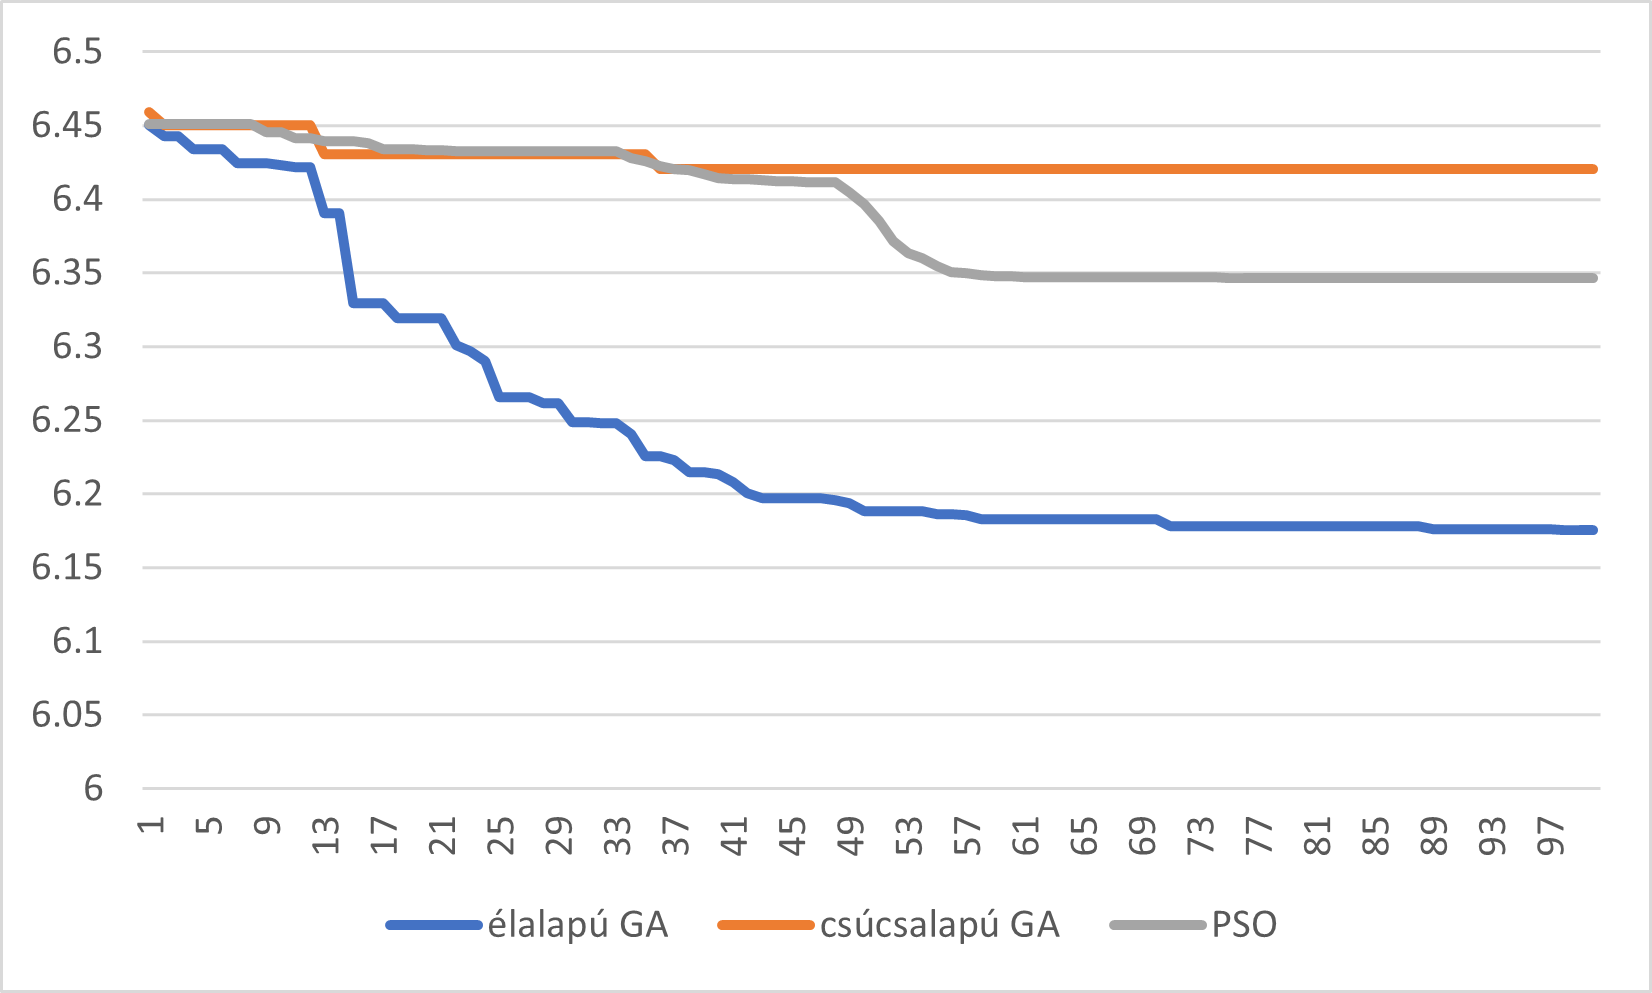
\includegraphics[width=0.30\linewidth]{init-spring-max-cost}}
	\subfigure[Véletlen inicializálás]{
		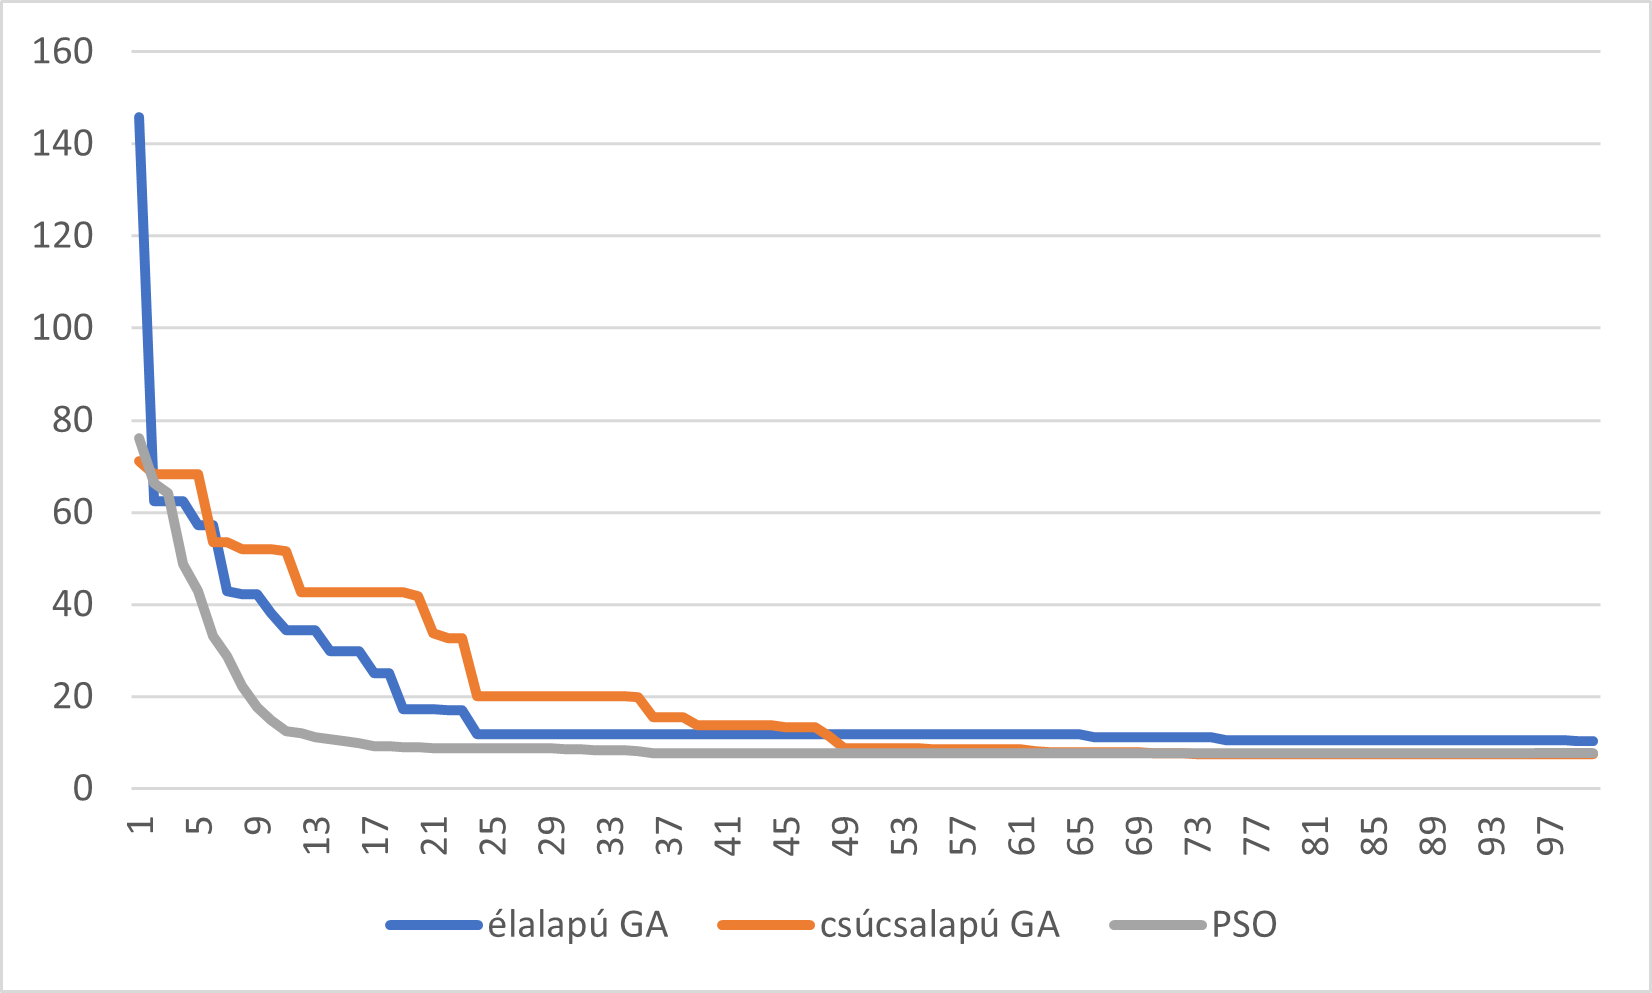
\includegraphics[width=0.30\linewidth]{init-rand-mean-cost}}
	\hspace{5pt}
	\subfigure[Élalapú inicializálás]{
		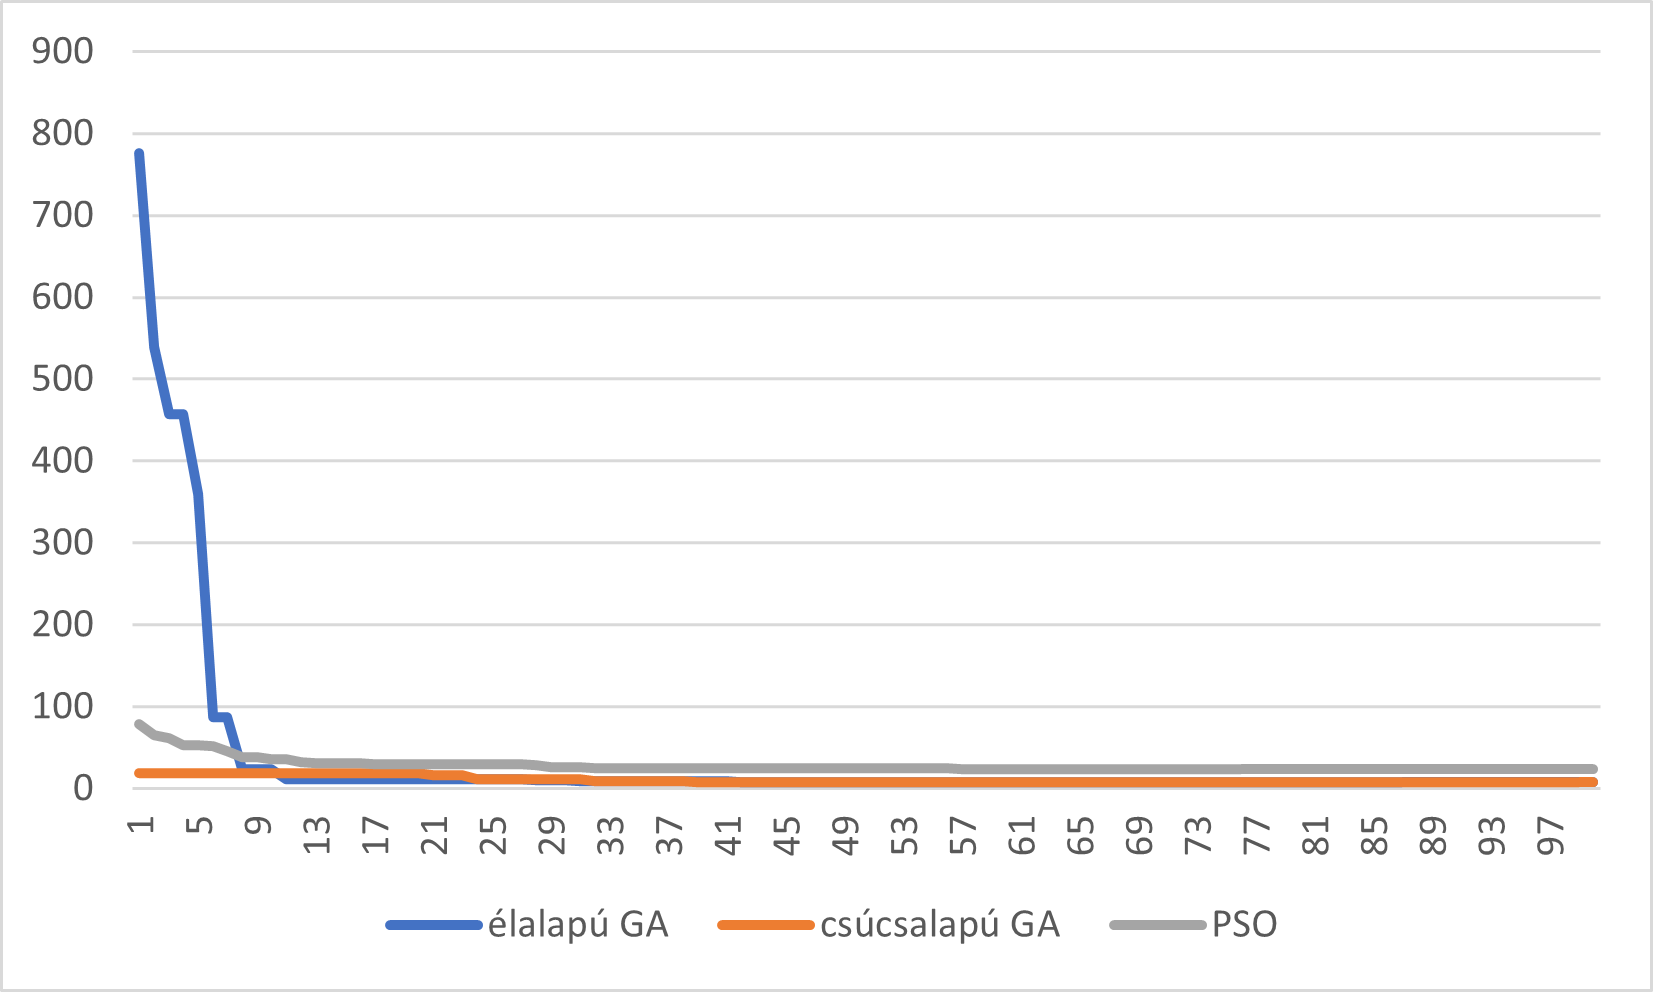
\includegraphics[width=0.30\linewidth]{init-edge-mean-cost}}
	\hspace{5pt}
	\subfigure[Erőalapú inicializálás]{
		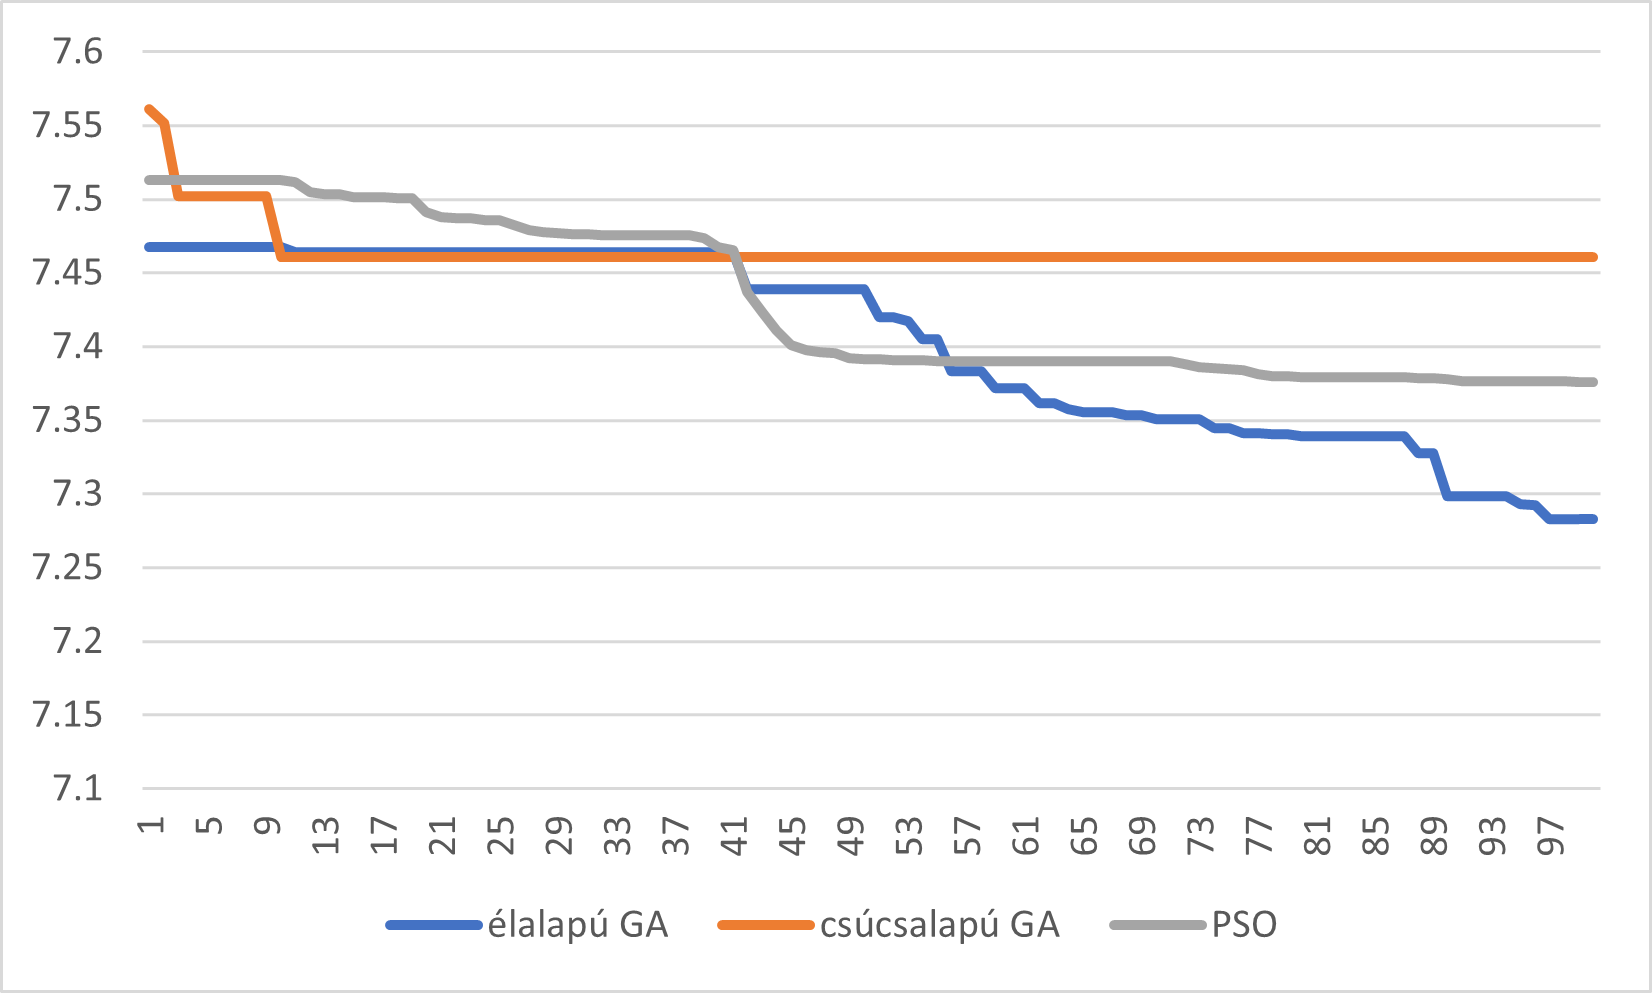
\includegraphics[width=0.30\linewidth]{init-spring-mean-cost}}
	\caption{Inicializálás min, max és átlagos $d$ értékekkel - költségfüggvények}
\end{figure}


\subsubsection{Hibrid inicializálási módszerek}

\subsection{Alternatív heurisztikák}
% TODO rigid / property is!!!!
% TODO szemantikai helyesség!!!!

% azok a heurisztikák, amik egy célhoz közelítve csökkenek, kívül kéne legyene a koundaryken

\subsection{Dinamikus költségfüggvény}


\subsection{Megoldások átvitele}


\subsection{Hipergráf konvolúciós hálózat}


\subsection{Futásidők}


% különböző méretű problémák (élek, csúcsok, mindkettő változtatása, élméretek)
% tanulás sebessége, változás méretarányosan
% helyettesítő heurisztikák összehasonlítása (tulajdonságok, skálák, helyettesítők) (futásidő)
% inicializálási módszerek & paraméterek
% opt módszerek & paraméterek
% transfer learning
% distance-ek fixálása (minden egy szegmensből áll) <- modellt kell átírni
% nem kirajzolható hipergráf
% evaluator paraméterezés
% mean & std a többi megoldásra az optimizer populációjában (mennyire stabil a tanulás, csak véletlen, vagy minden növekszik?)

\subsection{Összefoglalás}

\cleardoublepage
\chapter{Konklúzió}

% 11-ig - 60
% 11-ig öf - 2-5